\documentclass[11pt,oneside,a4paper]{report}

\usepackage[utf8]{inputenc}

\usepackage{amsfonts}
\usepackage{mdframed}
\usepackage{bussproofs}
\usepackage{standalone}
\usepackage{amsmath}
\usepackage{mathtools}
\usepackage{hyperref}
\usepackage{listings}
\usepackage{float}
\usepackage[english]{babel}
\usepackage{cleveref}
\usepackage{amsthm}
\usepackage{fancybox}
\usepackage{amsmath}
\usepackage{caption}
\usepackage{subcaption}
\usepackage{tikz}
\usepackage{pgfplots}
\usepackage{algorithmic}
\usepackage{algorithm}
\usepackage{float}
\usepackage{xcolor}
\usepackage{wrapfig}

\usepackage[style=alphabetic]{biblatex}
\addbibresource{bib.bib}

\usetikzlibrary{matrix,fit,trees,arrows,arrows.meta,positioning,shapes}
\tikzset{
  mtx/.style={
          inner sep=-\pgflinewidth,
          matrix of math nodes,
          column sep=-\pgflinewidth,
          nodes={
              draw=black,
              font=\color{black},
              minimum size=.75cm,
              anchor=center
          }
      },
  treenode/.style = {align=center, inner sep=0pt, text centered,
    font=\sffamily},
  arn_b/.style = {treenode, circle, white, font=\sffamily\bfseries, draw=black,
    fill=black, text width=1.5em},% arbre rouge noir, noeud noir
  arn_n/.style = {treenode, circle, black, draw=black,
    fill=none, text width=1.5em},% arbre rouge noir, noeud noir
  arn_r/.style = {treenode, circle, red, draw=red, 
    text width=1.5em, very thick},% arbre rouge noir, noeud rouge
  arn_l/.style = {treenode, circle, black, draw=none, 
    fill=none, text width=1.5em},% arbre rouge noir, noeud rouge
  arn_x/.style = {treenode, rectangle, draw=black,
    minimum width=0.5em, minimum height=0.5em}% arbre rouge noir, nil
}

\DeclarePairedDelimiter{\ceil}{\lceil}{\rceil}
\DeclarePairedDelimiter{\floor}{\lfloor}{\rfloor}

\theoremstyle{plain}
\newtheorem{lemma}{Lemma}[section]
\newtheorem{theorem}{Theorem}[section]

\newtheoremstyle{case}{}{}{}{}{}{:}{ }{}
\theoremstyle{case}
\newtheorem{case}{Case}

\newenvironment{pcases}[0]{
    \setcounter{case}{0}
    \begin{list}{}{}
}{\end{list}}

\newcommand{\pcase}[1]{
  \vspace*{-0.5cm}
    \item \begin{case}
            #1
    \end{case}
}

\newcommand{\eqtag}[1]{
    \stepcounter{equation}
    \tag{\theequation \hspace*{0.1cm} - #1}
}

\newcommand{\wherecase}[1]{
  \texttt{whe}&\texttt{re #1}
}
\newcommand{\spacecase}[0]{
  \tag*{}\\
}
\newcommand{\extracase}[1]{
  &\hspace{0.62cm}\texttt{#1}
}
\newcommand{\letexp}[3]{
  \texttt{let } \textit{#1 } = #2 \texttt{ in } #3
}

\mdfdefinestyle{style1}{leftmargin=-0.5cm,rightmargin=-0.5cm,skipbelow=1cm,skipabove=1cm,
   innertopmargin=0pt}
\mdfdefinestyle{style2}{leftmargin=-0.5cm,rightmargin=-0.5cm,skipbelow=1cm,skipabove=1cm,
   innertopmargin=0pt}
\mdfdefinestyle{bigbox}{leftmargin=-2cm,rightmargin=-2cm,skipbelow=1cm,skipabove=1cm,
   innertopmargin=0pt}
\mdfdefinestyle{bigbigbox}{leftmargin=-3.3cm,rightmargin=-3.3cm,skipbelow=1cm,skipabove=1cm,
   innertopmargin=0pt}

\makeatletter
\newenvironment{CenteredBox}{% 
\begin{Sbox}}{% Save the content in a box
\end{Sbox}\centerline{\parbox{\wd\@Sbox}{\TheSbox}}}% And output it centered
\makeatother
\theoremstyle{definition}
\newtheorem{exmp}{Example}[section]
\newtheorem{remark}{Remark}[section]

\def\exmpautorefname{Example}
\def\remarkautorefname{Remark}
\def\caseautorefname{Case}

\lstset{
    basicstyle=\ttfamily,
    numbers=left,
    showstringspaces=false,
    tabsize=1,
    frame=tbrl
}

\newfloat{lstfloat}{htbp}{lop}


\begin{document}
\begin{titlepage}
	\begin{center}
		\vspace*{1cm}
		\huge{Aspects of efficiency in functional programming languages}

		\vspace*{0.5cm}
		\large{by}

		\vspace{0.5cm}
		\Large{Samuel Valdemar Grange}

		\vspace*{0.5cm}
		\normalsize{supervised by}

		\vspace{0.5cm}
		\large{Prof. Kim Skak Larsen}

		\vfill

		\vspace*{0.7cm}
		
\includegraphics[width=0.4\textwidth]{sdulogo}

		\vspace*{1cm}
		\MakeUppercase{University of southern Denmark}

		\vspace*{0.3cm}
		\MakeUppercase{Department of mathematics and computer science}

		\vspace*{0.3cm}
		\large{Master's thesis in Computer Science}
	\end{center}

\end{titlepage}

\tableofcontents

\clearpage


\subsection{Notation}
Some functions are written in pattern matching style.
Functions which have parameters that can take different values or shapes, can implement a case for each value or shape.
For instance, a function which finds the cardinality of a set can be implemented as in \autoref{eq:notation:card}.
\begin{align}
  \texttt{card($\emptyset$) }&\texttt{= 0} \label{eq:notation:card} \\
  \texttt{card(\{x\} $\cup$ S) }&\texttt{= 1 + card(S)} \tag*{}
\end{align}
Inevitably, to allow complicated functions, like algorithms, some functions may require subexpressions.
Subexpressions are denoted with \texttt{where} when some expression is a composite of multiple expressions like in \autoref{eq:notation:fib}.
\begin{align}
  \texttt{fib(0) }&\texttt{= 0} \label{eq:notation:fib} \\
  \texttt{fib(1) }&\texttt{= 1} \tag*{} \\
  \texttt{fib(n) }&\texttt{= F$_\texttt{n-1}$ + F$_\texttt{n-2}$} \tag*{} \\
  \wherecase{F$_\texttt{n-1}$ = fib(n - 1)},\tag*{}\\
  \extracase{F$_\texttt{n-2}$ = fib(n - 2)}\tag*{}
\end{align}
Functions can also contain nested functions such as in \autoref{eq:nested}.
\begin{align}
  \texttt{double(n) }&\texttt{= k + id(n)} \label{eq:nested} \\
  \wherecase{id(x) = x,} \tag*{}\\
  \extracase{k = id(n)} \tag*{}
\end{align}
Finally, conditional cases may also occur in functions such that the choice of action is dependent on a predicate.
The function in \autoref{eq:cases} increments \texttt{n} in the case that it is even, else it returns \texttt{n}.
\begin{align}
  \texttt{makeOdd(n) }&\texttt{=} 
  \begin{cases}
    \texttt{n + 1} & \texttt{ if n \texttt{mod} 2 = 0 }\\
    \texttt{n} & 
  \end{cases}\label{eq:cases} 
\end{align}


\subsection{Running and sources}
The compiler and interpreter for the programming language implemented in this thesis was written in Scala.
To compile the compiler and interpreter, one must install sbt (simple build tool) and bloop (build server).
To run a compile and run a program the program bloop must be invoked with the arguments \texttt{bloop run root -- /path/to/code/src/L/fib}, where the absolute path is the path to the file containing the code for the implemented programming language.
Every resource required for this thesis can be found in the git repository at \url{https://github.com/valdemargr/masters}.



%\part{Compilers and languages}

\documentclass[11pt,oneside,a4paper]{report}

\begin{document}

\chapter{Programming languages}\label{sec:prog}
Computers are devices which read a well-defined, finite sequence of simple instructions and emit a result.
In theoretical analysis of computers, models have been developed to understand and prove properties.
A finite sequence of instructions fed to a computer is called an \textit{algorithm}, which is the language of high-level computation~\cite{copeland1997church}.
In modern encodings of algorithms or programs, ``high-level'' languages are used instead of the computational models.
Such languages are then translated into instructions that often are much closer to a computational model.
The process of translating programs into computer instructions is called \textit{compiling}, or \textit{transpiling} if the program is first translated into another ``high-level'' language.

For the purpose of this thesis, a simple programming language has been implemented to illustrate the concepts in detail.
The language transpiles to \textit{untyped lambda calculus}.
For the remainder, the language will be referred to as $L$.

\documentclass[11pt,oneside,a4paper]{report}

\begin{document}
\clearpage
\section{Untyped lambda calculus}\label{sec:lc}
The \textit{untyped lambda calculus} is a model of computation, developed by Alanzo Church\cite{church1936unsolvable}.
The untyped lambda calculus is a simple tangible language of just three terms.
\begin{align}
  &x
  \label{lc:lang:var}\\
  &\lambda x . E
  \label{lc:lang:abs}\\
  &Y E
  \label{lc:lang:app}
\end{align}
The first term is that of a \textit{variable} (\autoref{lc:lang:app}).
A variable is a reference to another lambda abstraction.
\autoref{lc:lang:abs} shows a lambda \textit{abstraction}, which contains a \textit{bound} variable $x$ and another lambda term $E$.
A bound variable is one explicitly parameterized in the abstraction.
In traditional programming languages bound variables are parameters to a function, whereas \textit{free} variables are variables that exist outside of the function scope.
It is easy to see that variables are either free or bound.
Free varables are determined by \autoref{eq:freevarvar}, \autoref{eq:freevarabs} and \autoref{eq:freevarapp}.
\begin{align}
    \label{eq:freevarvar}
    &Free(x) = \{ x \}\\
    \label{eq:freevarabs}
    &Free(\lambda x . E) = Free(E) \backslash \{ x \}\\
    \label{eq:freevarapp}
    &Free(Y E) = Free(Y) \cup Free(E)
\end{align}
Finally, in \autoref{lc:lang:app}, \textit{application}.
An application of two terms can be interpreted as substituting the variable in the left abstraction $Y$ with the right term $E$.
It is also common to introduce the \textit{let binding} to lambda calculus, which will be done when introducing typing in \autoref{sec:typing}.

\begin{exmp}
\label{ex:application}
Let $Y$ be $\lambda x . T$ and $E$ be $z$, then $Y E$ is $(\lambda x . T) z$.
Furtermore, substituteing $x$ for $E$, such that $Y$ becomes $T[x := E]$.
Since $E = z$, substitute $E$ for $z$, such that $T[x := z]$, read as ``Every instance of $x$ in $T$, should be substituted by $z$''.
\end{exmp}
\begin{remark}
Substituting lambda terms is a popular method of evaluateing lambda calculus programs.
    Languages like Miranda, Clean and general purpose evaluation programs like the G-machine \autoref{needscitation}, implement \textit{graph rewriting}, which will be introduced in \autoref{sec:graphrewriting}
\end{remark}

The untyped lambda calculus is in fact turing complete; any algorithm that can be evaluated by a computer can be encoded in the untyped lambda calculus.
The turing completeness of the untyped lambda calculus can be realized by modelling numerics, boolean logic and recursion with the \textit{Y-combitator}.
Church encoding, is the encoding of numerics, arithmetic expressions and boolean logic~\cite{church1985calculi}.
For the remainder of the dissertation, ordinary arithmetic expressions are written in traditional mathematics.
The expressiveness and simplicity of lambda calculus, makes it an exellent language to transpile to, which in fact, is a common technique.

\section{Translation to lambda calculus}
High level languages associated with lambda calculus are often also very close to it.
The $L$ language is very close to the untyped lambda calculus.
See two equivalent programs, \autoref{lc:add} and \autoref{lst:add}, that both add an $a$ and a $b$.
\begin{align}
(\lambda add . E)(\lambda a . (\lambda b . a + b))
\label{lc:add}
\end{align}
\begin{CenteredBox}
    
\end{CenteredBox}
\begin{lstlisting}[language=ML,caption={Add function},label={lst:add}]
fun add a b = a + b;
\end{lstlisting}
Notice that in \autoref{lc:add} the term $E$ is left undefined, $E$ is ``the rest of the program in this scope''.
If the program was to apply $1$ and $2$ to add, directly below in the high level representation (\autoref{lst:addapp}) the lambda calculus equivalent would look like \autoref{lc:addapp}.
\begin{align}
    (\lambda add . add \,\, 1 \,\, 2)(\lambda a . (\lambda b . a + b))
\label{lc:addapp}
\end{align}
\begin{lstlisting}[language=ML,caption={Add function applied},label={lst:addapp}]
fun add a b = a + b;
add 1 2;
\end{lstlisting}

\subsection{Scoping}\label{scoping}
Notice that \autoref{lc:add}, must bind the function name ``outside the rest of the program'' or more formally in an outer scope.
In a traditional program such as \autoref{lst:traditional}, functions must be explicitly named to translate as in the above example.
\begin{lstlisting}[language=ML,caption={A traditional program},label={lst:traditional}]
fun add a b = a + b;
fun sub a b = a - b;
sub (add 10 20) 5;
\end{lstlisting}
\begin{lstlisting}[language=ML,caption={An order dependant program},label={lst:orddep}]
fun sub a b = add a (0 - b);
fun add a b = a + b;
sub (add 10 20) 5;
\end{lstlisting}
Notice that there are several problems, such as, the order of which functions are defined may alter whether the program is correct or not.
For instance, the program defined in \autoref{lst:orddep} would not translate correct, it would translate to \autoref{lc:orddep}.
The definition of $sub$, or rather, the applied lambda abstraction, is missing a reference to the $add$ function.
\begin{align}
(\lambda sub . (\lambda add . (sub \,\, (add \,\, 10 \,\, 20) \,\, 5)) \,\, (\lambda a . (\lambda b . a + b))) \,\, (\lambda a . (\lambda b . add \,\, a (0 - b)))
\label{lc:orddep}
\end{align}

\textit{lambda lifting} is a technique where free variables (\autoref{sec:lc}), are explicitly parameterized~\cite{johnsson1985lambda}.
%A free variable, is a variable in respect to some function $f$ that is referenced from within $f$, but defined outside. 
This is exactly the problem in \autoref{lc:orddep}, which has the lambda lifted solution \autoref{lc:ordfix}.
\begin{align}
(\lambda sub . (\lambda add . (sub \,\, add \,\, (add \,\, 10 \,\, 20) \,\, 5)) \,\, (\lambda a . (\lambda b . a + b))) \,\, (\lambda add .(\lambda a . (\lambda b . add \,\, a (0 - b))))
\label{lc:ordfix}
\end{align}
As it will turn out, this will also enables complicated behaviour, such as \textit{mutual recursion}.

Moreover, lambda lifting also conforms to ``traditional'' scoping rules.
\textit{Variable shadowing} occurs when there exists $1 < $ reachable variables of the same name, but the ``nearest'', in regard to scope distance is chosen.
Effectively, other variables than the one chosen, are \textit{shadowed}.
Variable shadowing is an implied side-effect of using using lambda calculus.
Convince yourself that the function $f$ in \autoref{lst:scoping}, yields $12$.
\begin{lstlisting}[language=ML,caption={Scoping rules in programming languages},label={lst:scoping}]
let x = 22;
let a = 10;
fun f = 
  let x = 2;
  a + x;
\end{lstlisting}

\subsection{Recursion}
%Complexity - ``The state or quality of being intricate or complicated''
%\\\\
\noindent Reductions in mathematics and computer science are one of the principal methods used for developing beautiful equations and algorithms.
\begin{lstlisting}[language=ML,caption={Infinite program},label={lst:infprog}]
fun f n = 
  if (n == 0) n
  else if (n == 1) n + (n - 1)
  else if (n == 2) n + ((n - 1) + (n - 2))
  ...
\end{lstlisting}
\autoref{lst:infprog} defines a function $f$, that in fact is infinite.
Looking at the untyped lambda calculus, there are not any of the three term types that define infinite functions or abstractions, at first glance.
Instead of writing an infinite function, the question is rather, how can a reduction be peformed on this function, such that it can evaluate \textit{any} case of $n$?
\begin{lstlisting}[language=ML,caption={Recursive program},label={lst:recprog}]
fun f n = 
  if (n == 0) n
  else n + (f (n - 1))
\end{lstlisting}
\autoref{lst:recprog} defines a recursive variant of $f$, it is a product of the reduction in \autoref{eq:fred}.
\begin{align}
    n + (n - 1) \dots + 0 = \sum_{k = 0}^n k
    \label{eq:fred}
\end{align}
But since the untyped lambda calculus is turing complete, or rather, if one were to show it were,
it must also realize algorithms that are recursive or include loops, the two of which are equivalent in expressiveness.
\begin{align}
    (\lambda f . E) (\lambda n . \texttt{if} (n == 0) (n) (n + (f (n - 1))))
    \label{eq:naiverec}
\end{align}
The naive implementation of a recursive variant, will yield an unsolvable problem, in fact, an infinite problem.
In \autoref{eq:naiverec}, when $f$ is applied recursively, it must be referenced.
How can $f$ be referenced, if it is ``being constructed''?
Substituting $f$ with its implementation in \autoref{eq:naiverecdepth}, will yield the same problem again, but at one level deeper.
\begin{align}
    (\lambda f . E) (\lambda n . \texttt{if} (n == 0) (n) (n + ((\lambda n . \texttt{if} (n == 0) (n) (n + (f (n - 1)))) (n - 1))))
    \label{eq:naiverecdepth}
\end{align}
One could say, that the problem is now recursive.
Recall that lambda lifting (\autoref{scoping}), is the technique of explicitly parameterizing outside references.
Convince yourself that $f$ lives in the scope above its own body, such that, when referenceing $f$ from within $f$, $f$ should be parameterized as in \autoref{lst:erec}, translating to \autoref{eq:erec}.
\begin{lstlisting}[language=ML,caption={Explicitly passing recursive function},label={lst:erec}]
fun f f n = 
  if (n == 0) n
  else n + (f f (n - 1))
\end{lstlisting}
\begin{align}
    (\lambda f . E) (\lambda f . (\lambda n . \texttt{if} (n == 0) (n) (n + (f \,\, f \,\, (n - 1)))))
    \label{eq:erec}
\end{align}
The initial invocation of $f$, must involve $f$, such that it becomes $f \,\, f \,\, n$.
The \textit{Y-combinator}, an implementation of a fixed-point combinator, in \autoref{eq:ycomb} is the key to realize that the untyped lambda calculus can implement recursion.
Languages with functions and support binding functions to parameters, can implement recursion with the Y-combinator.
\begin{align}
    \lambda f . (\lambda x . f (x x)) (\lambda x . f (x x))
    \label{eq:ycomb}
\end{align}

Implementing mutual recursion is an interesting case of lambda lifting and recursion in untyped lambda calculus.
\begin{lstlisting}[language=ML,caption={Mutual recursion},label={lst:mutrec}]
fun g = f;
fun f = g;
\end{lstlisting}
Notice in \autoref{lst:mutrec} that $g$ requires $f$ to be lifted and $f$ requires $g$ to be lifted.
If a translation ``pessimistically'' lifts all definitions from the above scope, then all required references exist in lexical scope.
\\\\
Languages have diffirent methods of introducing recursion, some of which have very different implications, especially when considering types.
For instance, OCaml has the \texttt{let rec} binding, to introduce recursive definitions.
The \texttt{rec} keyword indicates to the compiler that the binding should be able to ``see itself'' (\autoref{typing}).



\end{document}


\documentclass[11pt,oneside,a4paper]{report}

\begin{document}
\section{High level abstractions}\label{sec:highlevel}
The lambda calculus is a powerful language that can express any algorithm.
Expressiveness does not necessarily imply ergonomics or elegance, in fact encoding moderately complicated algorithms in lambda calculus becomes quite messy.

\subsection{Algebraic data types}
\label{sec:adt}
Algebraic data types, in their essence, are tagged unions of tuples.
Algebraic data types become much more powerful once enhanced with \textit{type constructors}, as such, they are closely related to types thus require some type theory to fully grasp.
Types are explored more in depth in \autoref{sec:types}.

An algebraic data type is a name $A$ for a tagged union of tuples $T_1, T_2 \dots , T_n$ that states that any tuple $T_k$ with tag $t_k$ for some $1 \leq k \leq n$ is of type $A$.
This construct allows any of the tuples $T_1, T_2 \dots , T_n$ to be unified and inhabit $A$ under the names $t_1, t_2 \dots , t_n$.

In $L$, algebraic data types give rise to tangible implementations of abstract types such as lists (\autoref{lst:listadt:int}).
\autoref{lst:listadt:int} displays an algebraic data type with name \texttt{IntList} which is the tagged union of the nullary tuple \texttt{Nil} and the binary tuple \texttt{Cons}.
\texttt{IntList} states that if a value that inhabits the type \texttt{IntList} occurs, it must either be the tag \texttt{Nil} or the tag \texttt{Cons} which carries a value of type \texttt{Int} and another value of type \texttt{IntList}.
\begin{figure}
\begin{lstlisting}[language=ML,caption={List algebraic data type},label={lst:listadt:int}]
type IntList = 
    | Nil
    | Cons Int IntList
;
\end{lstlisting}
\end{figure}
%\begin{figure}
%\begin{lstlisting}[language=ML,caption={List algebraic data type},label={lst:listadt}]
%type List a = 
    %| Nil
    %| Cons a (List a)
%;
%\end{lstlisting}
%\end{figure}
%%\autoref{lst:listadt} is an implementation of a linked list. 
%The list value can either take the type of \texttt{Nil} indicating an empty list, or it can take the type of \texttt{Cons} indicating a pair of type $a$ and another list.
%The list implementation has two constructors and one type parameter.
%The type parameter $a$ of the list algebraic data type defines a \textit{polymorphic type}; $a$ can agree on any type, it is universally quantified \texttt{$\forall a. $ Cons $a$ (List $a$)}.
%The two constructors \texttt{Nil} and \texttt{Cons} both create a value of type \texttt{List a} once instatiated.
\begin{figure}
\begin{lstlisting}[language=ML,caption={List instance and match},label={lst:listinstance}]
fun main =
  let l = Cons 1 (Cons 2 (Cons 3 Nil));
  match l 
      | Nil -> 0;
      | Cons x xs -> x;
  ;
\end{lstlisting}
\end{figure}
Once a tuple of values are embedded by a tag into an algebraic data type, such as a list, it must be extractable, to be of any use.
Values of algebraic data types are extracted and analysed with \textit{pattern matching}.
Pattern matching comes in many forms, notably it may allow one to define a computation based on the type an algebraic data type instance realizes (\autoref{lst:listinstance}), which is the type of pattern matching of $L$.

\subsubsection{Scott encoding}
Pattern matching strays far from the simple untyped lambda calculus, but can in fact be encoded into it.
\textit{scott encoding} (\autoref{se:general}) is a technique that describes a general purpose framework to encode algebraic data types into the lambda calculus~\cite{scott1962system}.
Considering an algebraic data type instance as a function which accepts a set of ``handlers'', paves the way for the encoding into the lambda calculus.
The scott encoding specifies that constructors should now be functions that are each parameterized by the constructor parameters $x_1 \dots x_{A_i}$ where $A_i$ is the arity of the constructor $i$.
Additionally, each of the constructor functions return a $n$ arity function, where $n$ is the number of tagged tuples $T_1, T_2 \dots , T_n$.
Of the $n$ functions, the constructor parameters $x_1 \dots x_{A_i}$ are applied to the $i$'th ``handler'' $c_i$.
These encoding rules ensure that the ``handler'' functions are provided uniformly to all instances of the algebraic data type.
\begin{align}
    \lambda x_1 \dots x_{A_i}. \lambda c_1 \dots c_n. c_i x_1 \dots x_{A_i}
\label{se:general}
\end{align}
\begin{exmp}
    The \texttt{IntList} algebraic data type in \autoref{lst:listadt:int} has two constructors, the \texttt{Nil} constructor and the \texttt{Cons} constructor.
    The construction of a value of type \texttt{Cons} or \texttt{Nil} effectively partially applies an abstraction and returns an abstraction that is uniform for both \texttt{Nil} and \texttt{Cons}, such as in (\autoref{lst:listscott}).
    %\autoref{eq:nilconstructor} is in fact also the type of \texttt{List} once instantiated, effetively treating partially applied functions as data.
\begin{figure}
\begin{lstlisting}[language=ML,caption={List algebraic data type implementation},label={lst:listscott}]
fun cons x xs = 
    fun c onNil onCons = onCons x xs;
    c;

fun nil = 
    fun c onNil onCons = onNil;
    c;
\end{lstlisting}
\end{figure}

Types have not been introduced yet, but seeing the types of these functions might help understanding scott encoding.
\autoref{eq:nilconstructor} is the constructor type for \texttt{Nil} and \autoref{eq:consconstructor} is the constructor type for \texttt{Cons}.
\begin{align}
   &b \rightarrow (a \rightarrow \texttt{List } a \rightarrow b) \rightarrow b
   \label{eq:nilconstructor}\\
   &(a \rightarrow \texttt{List } a \rightarrow b) \rightarrow b \rightarrow (a \rightarrow \texttt{List } a \rightarrow b) \rightarrow b
   \label{eq:consconstructor}
\end{align}

Encoding the constructors in $L$ yields the functions defined in \autoref{lst:listscott}.
Pattern matching is but a matter of applying the appropriate handlers.
In \autoref{lst:listscottexample}.
\begin{lstlisting}[language=ML,caption={Example of scott encoded list algebraic data type},label={lst:listscottexample}]
fun main =
  let l = cons 1 (cons 2 (cons 3 nil));
  fun consCase x xs = x;
  fun nilCase = 0;
  l consCase nilCase
\end{lstlisting}
\end{exmp}

%Efficiency can be a bit tricky in lambda calculus as it is at the mercy of implementation.
%A common method of considering efficiency is counting \textit{$\beta$-reduction} since they evaluate to function invocations.
%The $\beta$-reduction is a substitution which substitutes an application where the left side is an abstraction in witch the bound variable is substituted with the right side term (\autoref{eq:betareduction}). 
%\begin{align}
    %&\beta_{red}((\lambda x . T) E) = T[x := E]
   %\label{eq:betareduction}
%\end{align}
%It should be clear that invoking a $n$ arity function will take $n$ applications.
%In the case of a scott encoded algebraic data types the largest term in regard to complexity is either the size of the set of ``handler'' functions or the ``handler'' function with most parameters.
%The time to evaluate pattern match is thus $O(\max_i(c_i + A_i))$.



\end{document}


\end{document}


\documentclass[11pt,oneside,a4paper]{report}

\begin{document}

\chapter{Typing and validation}
Automatic validation is one of many reasons to use computers for solving various tasks including writing new computer programs.
Spellchecking is a very common and trivial instance of an input validation algorithm. 
The equivalent for computer programs could be type checking; the problem of validating a programmers intuition of a program's intent.

\documentclass[11pt,oneside,a4paper]{report}

\begin{document}
\section{Types and validation}
\label{sec:types}
The spell checking equivalent for computer programs could be type checking; a subproblem of validating a programmer's intuition of a program's intent.
Types also have other properties than simply validating they can in fact be related to theorems to which an implementation is the proof~\cite{howard1980formulae}.
\begin{lstlisting}[language=ML,caption={Head implementation},label={lst:headimpl},mathescape=true]
$\texttt{fun head l: List a} \rightarrow \texttt{a =}$
    $\texttt{match l}$
        $\texttt{| Cons x \_ } \rightarrow \texttt{x;}$
        $\texttt{| Nil} \rightarrow \texttt{?;}$
    ;
\end{lstlisting}
For instance, consider the implementation of the fuction with type $\texttt{List a} \rightarrow \texttt{a}$ in \autoref{lst:headimpl}.
A total implementation of the function cannot exist.

The type system for the $L$ language will be the Hindley-Milner type system~\cite{hindley1969principal,milner1978theory}.

\subsection{The language of types}
Before delving into types, the lambda calculus defined in \autoref{sec:lc} must be augmented with the \textit{let expression} (\autoref{eq:letb}).
\begin{align}
	\texttt{let } x = Y \texttt{ in } E
	\label{eq:letb}
\end{align}
It should be noted that the let binding can be expressed by abstraction and application (\autoref{eq:letaa}).
\begin{align}
	(\lambda x . E) (Y)
	\label{eq:letaa}
\end{align}
The let expression has a nice property that will become apparent later when typing rules are introduced.

Types are an artificial layer atop of a program just as spell checking is an artificial layer atop text.
There are two variants of types in the Hindley-Milner type system, the \textit{monotype} and the \textit{polytype}.
A monotype is either a type variable, an abstraction of two monotypes or an application of a type constructor (\autoref{eq:mono}).
\begin{align}
	mono \,\,\tau = a \,|\, \tau \rightarrow \tau \,|\, C \tau_1 \dots \tau_n
	\label{eq:mono}
\end{align}
\textit{Atoms} are terminal terms in a formula and are expressed either by type variable $a$ or $C$ with no type parameters.
The application term of the monotype is dependent on the primitive types of the programming language.
The types $\tau_1 \dots \tau_n$ are monotype parameters required to construct some type $C$.
In $L$ the set of type constructors are $\{ \texttt{Int}, \texttt{Bool} \} \cup \texttt{ADT}$.
\texttt{Int} and \texttt{Bool} are type constructors of arity 0 thus only have one instantiation and are atomic.
The set of constructors \texttt{ADT} encapsulates the set of program defined algebraic data structures (\autoref{adts}).
\begin{exmp}
    Let $\texttt{ADT} = \{ \texttt{List} \}$ where \texttt{List} is defined as in \autoref{lst:listadt}.
    The \textit{type constructor} (not to be confused for constructors like \texttt{Cons} or \texttt{Nil}) for \texttt{List} has the signature $\texttt{a} \rightarrow \texttt{List a}$ stating that if supplied with some type \texttt{a} it constructs a type of \texttt{List a} (effectively containing the provided type).
    The type \texttt{List} is a type constructor with one type parameter \texttt{a}.
\end{exmp}

$\bot$ denotes falsity, in type systems a value of this type can never exist since that in itself would disprove the program.
It is common in programming languages with strong type systems to let thrown exceptions be of type $\bot$ since it adheres to every type and indicates that the program is no longer running, since no instance of $\bot$ can exist.
$\top$ denotes truth, in type systems every type is a supertype of $\top$.
$\top$ is in practice only used to model side effects, since not all side effects return useful values.
In programming languages with side effects $\bot$ and $\top$ are considerably more useful than in pure programming languages.

A polytype is a polymorphic type (\autoref{eq:poly}).
\begin{align}
	poly \,\, \sigma = \tau \,|\, \forall a . \sigma
	\label{eq:poly}
\end{align}
Polymorphic types either take the shape of a type variable or introduce a type which all types $a$ adhere to. 
This does not necessarily include \textit{all} types since the \textbf{Gen} rule of \autoref{fig:hmrules} constrains the domain that $a$ ranges over to contain only type variables that are not free.
Many types may adhere to a polymorphic type but polymorphic types do not adhere to any type other than polymorphic types.
The concept of adherence in types is commonly called \textit{subtyping}.
Every subtype is a \textit{at least} an implementation of it's supertype.
Since this concept can be difficult to grasp from just text, observe \autoref{fig:polytree}.
\begin{figure}[ht]
    \centering
        \begin{tikzpicture}
            \node[draw=none] (sigma) {$\sigma$};

            \node[draw=none, below = of sigma] (top) {$\top$};

            \node[draw=none, below = of top] (tv) {$\tau$};
            \node[draw=none, left = of tv] (arr) {$\tau_1 \rightarrow \tau_2$};
            \node[draw=none, right = of tv] (tc) {$C \tau_1 \dots \tau_n$};

            \node[draw=none, below = of tv] (bot) {$\bot$};

            \path [->] (sigma) edge node[left] {} (top);

            \path [->] (top) edge node[left] {} (arr);
            \path [->] (top) edge node[left] {} (tv);
            \path [->] (top) edge node[left] {} (tc);

            \path [->] (tv) edge node[left] {} (bot);
            \path [->] (arr) edge node[left] {} (bot);
            \path [->] (tc) edge node[left] {} (bot);
        \end{tikzpicture}
    \caption{The type hierarchy of Hindley-Milner.}
    \label{fig:polytree}
\end{figure}
Note that $\sigma$ is controversial to introduce to the type hierarchy and has only been so to illustrate the point of subtyping.
$\sigma$ is but a mechanism to prove type systems, $\sigma$ is never a specific type.
\begin{remark}
    \label{remark:polyimpl}
An important implementation detail which should be noted is that of the polymorphic type.
Polymorphic types can be regarded as being a pair of bound types and monotype.
Instead of keeping track of what types cannot occur, keeping track of the ones than can occur simplifies the implementation.
This representation is convenient for the \textbf{Gen} rule.
\end{remark}

A principal component of typing in Hindley-Milner is the \textit{environment}.
The environment $\Gamma$ is a set of pairs of variable names and polytype (\autoref{eq:env}).
$\Gamma \vdash x: \sigma$ implies a \textit{typing judgment}, meaning that given $\Gamma$, the variable $x$ can take the type $\sigma$.
\begin{remark}
    \label{remark:judgpoly}
    Judging a type does not necessarily mean that the judged type is the only type that $x$ may take, it states that it is one \textit{possible} type that $x$ may take.
    The property of taking multiple possible types is what allows polymorphism.
    This is made more apparent in \autoref{exmp:letpoly} where \texttt{id} may take the type of either $\forall a . a \rightarrow a$, $\texttt{Int} \rightarrow \texttt{Int}$ or $\forall a . (a \rightarrow a) \rightarrow (a \rightarrow a)$.
\end{remark}
\begin{align}
	\Gamma \,\, = \epsilon \,|\, \Gamma, x : \sigma
	\label{eq:env}
\end{align}

Like in the untyped lambda calculus, types also have notions of free and bound type variables.
Bound type variables are ones that explicitly have been introduced to the type system by either let or abstraction in the context of some expression.
Type variables are bound when they have been introduced by a quantification or exist in the environment.
\begin{align}
	 & \textit{free}(a) = \{ a \}                                                              \\
	 & \textit{free}(C \tau_1 \dots \tau_n ) = \bigcup_{i = 1}^n \textit{free}(\tau_i)           \\
     & \textit{free}(\tau_1 \rightarrow \tau_2) = \textit{free}(\tau_1) \cup \textit{free}(\tau_2)          \\
	 & \textit{free}(\Gamma) = \bigcup_{x:\sigma \in \Gamma} \textit{free}(\sigma)             \\
	 & \textit{free}(\forall a . \sigma) = \textit{free}(\sigma) - \{ a \}                     
	 %& \textit{free}(\Gamma \vdash x : \sigma) = \textit{free}(\sigma) - \textit{free}(\Gamma)
\end{align}
\begin{exmp}
Consider the type for the function \texttt{fst} in \autoref{lst:fstimpl}.
\begin{lstlisting}[language=ML,caption={First function},label={lst:fstimplbad},mathescape=true]
fun fst a b: $\forall$A.$\forall$B.A $\rightarrow$ B $\rightarrow$ A = a;
\end{lstlisting}
\begin{lstlisting}[language=ML,caption={First function in lambda calculus},label={lst:fstimpl},mathescape=true]
let fst = $\lambda$a.(let f = $\lambda$b.a in f) in fst
\end{lstlisting}
    The type for \texttt{fst} is $\forall A \forall B . A \rightarrow B \rightarrow A$.

    Note that a naive typing could look like $\forall A  . A \rightarrow (\forall B . B \rightarrow A)$ but rank-2 polymorphism is not typable in Hindley-Milner.
    An important realization is the context from where the type analysis is made.
    If type analysis is made from within the bounded context of \texttt{f} the type of \texttt{f} becomes $\forall B . B \rightarrow A$ and the type variable $A$ is free.
\end{exmp}
The variables which may appear in a quantification have an important role in \autoref{eq:substitution}, since only free variables may be substituted.
Free variables are also a core part of generalizing a type for inference algorithms (\autoref{subsec:algw}).
When modelling polymorphic types with a technique such as \autoref{remark:polyimpl} finding the set of bound variables is trivial.
\begin{align}
    & \textit{bound}(\tau) = \textit{free}(\tau) - \textit{free}(\Gamma)
\end{align}
When generalizing a type $\tau$ all types which do not occur in $\Gamma$ must be quantified.
\begin{exmp}
\begin{gather}
    \Gamma = \{ (\textit{x}, \gamma) \} \label{eq:monoeq}\\
\begin{align}
    \textit{bound}(\tau \rightarrow \gamma) &= \{\tau , \gamma\} - \textit{free}(\Gamma)\\
    &= \{\tau , \gamma\} - \{ \gamma \} = \{ \tau \}\tag*{}
\end{align}
\end{gather}
Clearly the only bound type variable in the context of $\tau \rightarrow \gamma$ is $\tau$ such that it may become $\forall \tau. \tau \rightarrow \gamma$ in the instance that the type represents a polymorphic let expression.
    Note that $\texttt{x:}\gamma$ in \autoref{eq:monoeq} does not contain $\gamma$ as a quantified type since it has been introduced by an abstraction and \textbf{Abs} only introduces monomorphic types (\autoref{fig:hmrules}).
    An interesting observation is that there can only exist one implementation of the above type system if $\tau \rightarrow \gamma$ is to be introduced by a polymorphic let expression which is displayed in \autoref{lst:theoremsforfree}~\cite{wadler1989theorems}.
\begin{lstlisting}[language=ML,caption={Implementation of type state},label={lst:theoremsforfree},mathescape=true]
$\lambda$x.
    let z = ($\lambda$y.x) in
    $\dots$
\end{lstlisting}
\end{exmp}

\section{Hindley-Milner}
With the now introduced primitives, the Hindley-Milner type system is but a set of rules composed by said primitives.
\begin{figure}[ht]
	\begin{mdframed}
		\minipage{0.49\textwidth}
		\begin{prooftree}
			\AxiomC{$x: \sigma \in \Gamma$}
			\LeftLabel{Var}
			\UnaryInfC{$\Gamma\vdash x:\sigma$}
		\end{prooftree}
		\endminipage
		\minipage{0.49\textwidth}
		\begin{prooftree}
			\AxiomC{$\Gamma \vdash e_1 : \tau_1 \rightarrow \tau_2$}
			\LeftLabel{App}
			\AxiomC{$\Gamma \vdash e_2 : \tau_1$}
			\BinaryInfC{$\Gamma \vdash e_1 e_2 : \tau_2$}
		\end{prooftree}
		\endminipage\hfill\vspace{0.8cm}

		\minipage{0.49\textwidth}
		\begin{prooftree}
			\AxiomC{$\Gamma, x: \tau_1 \vdash e : \tau_2$}
			\LeftLabel{Abs}
			\UnaryInfC{$\Gamma \vdash \lambda x . e : \tau_1 \rightarrow \tau_2$}
		\end{prooftree}
		\endminipage\hfill
		\minipage{0.49\textwidth}
		\begin{prooftree}
			\AxiomC{$\Gamma \vdash e_1 : \sigma$}
			\LeftLabel{Let}
			\AxiomC{$\Gamma ,x : \sigma \vdash e_2 : \tau$}
			\BinaryInfC{$\Gamma \vdash \texttt{let } x = e_1 \texttt{ in } e_2 : \tau$}
		\end{prooftree}
		\endminipage\hfill\vspace{0.8cm}

		\minipage{0.49\textwidth}
		\begin{prooftree}
			\AxiomC{$\Gamma \vdash e : \sigma_1$}
			\AxiomC{$\sigma_1 \sqsubseteq \sigma_2$}
			\LeftLabel{Ins}
			\BinaryInfC{$\Gamma \vdash e : \sigma_2$}
		\end{prooftree}
		\endminipage\hfill
		\minipage{0.49\textwidth}
		\begin{prooftree}
			\AxiomC{$\Gamma \vdash e : \sigma$}
            \AxiomC{$a \notin \textit{free}(\Gamma)$}
			\LeftLabel{Gen}
			\BinaryInfC{$\Gamma \vdash e : \forall a . \sigma$}
		\end{prooftree}
		\endminipage
	\end{mdframed}
	\caption{Hindley-Milner type rules}
	\label{fig:hmrules}
\end{figure}
There are six rules in the Hindley-Milner rules outlined in \autoref{fig:hmrules}.
\begin{itemize}
    \item \textbf{Var} states that if some variable $x$ with type $\sigma$ exists in the environment, the type can be judged.
        In practice, when $x: \sigma$ is encountered in the expression tree it is added to the environment.
    \item \textbf{App} decides that if $e_1 : \tau_1 \rightarrow \tau_2$ and $e_2 : \tau_1$ has been judged to exist then $e_1 e_2$ implies the removal of $\tau_1$ from $\tau_1 \rightarrow \tau_2$ such that $e_1 e_2: \tau_2$.
    \item \textbf{Abs} is the typing rule of lambda abstractions.
        If $x : \tau_1$ exists in the environment from some type analysis of $e$ and the abstraction's body $e$ has been judged to be of type $\tau_2$ then the abstraction of $x$ must take the type of $x$ to create the type of the body $e$.
    \item \textbf{Let} states that if $e_1$ has been judged to have type $\sigma$ then the let expression's identifier $x: \sigma$ must exist in the environment when deriving the type of $e_2$.
        Observe that \textbf{Let} introduces a polymorphic type to the environment while \textbf{Abs} introduces a monomorphic one.
        Note that by \autoref{remark:judgpoly} $x$ may be polymorphic in $e_2$.
    \item \textbf{Inst} specializes some polymorphic type (in regard to the type system implementation) to a more specific polymorphic type.
        $\sqsubseteq$ is the partial order of types where the binary relation between two types compares the descriptiveness of types.
        \begin{exmp}
            In $L$ the smallest element is the top of the type hierarchy (\autoref{fig:polytree}), the polymorphic type.
        \end{exmp}
    \item \textbf{Gen} generalizes over all bound variables $a$.
\end{itemize}
Let polymorphism is exemplified in \autoref{exmp:letpoly}.

\begin{exmp}
\label{exmp:letpoly}
Throughout this example the convenient syntax $(x, z)$ is the pair of the variables $x$ and $z$ which can be implemented by algebraic data structures or a combinator.

The identity function is a common example to illustrate type systems (\autoref{lst:idfun}).
\begin{lstlisting}[language=ML,caption={Identity function in $L$},label={lst:idfun}]
fun id x = x;
id 4;
\end{lstlisting}
\begin{lstlisting}[language=ML,caption={Identity function in lambda calculus with let},label={lst:idfunlam},mathescape=true]
let id = ($\lambda x . x$) in
id 4
\end{lstlisting}
Stating that id has the type $\forall a.a \rightarrow a$ and $4$ has the type \texttt{Int} is \autoref{lst:idfunlam} program correct?
By applying the Hindley-Milner rules one can prove or disprove this statement.
A correct proof of \autoref{lst:idfun} must be \autoref{fig:typeexampleid}.

\begin{lstlisting}[language=ML,caption={Identity function in lambda calculus by abstraction},label={lst:idfunlamabs},mathescape=true]
($\lambda$id.id 4)($\lambda$x.x)
\end{lstlisting}
\autoref{lst:idfunlam} and \autoref{lst:idfunlamabs} are two equivalent programs with slightly different proofs which raises the question of why the let expression is even needed.
If \autoref{lst:idfunlam} and \autoref{lst:idfunlamabs} were to be slightly changed such that two new programs \autoref{lst:idfunlam2} and \autoref{lst:idfunlamabs2} were to be proved, \autoref{lst:idfunlamabs2} would not be provable while \autoref{lst:idfunlam2} would.
\begin{lstlisting}[language=ML,caption={Identity function with two applications},label={lst:idfunlam2},mathescape=true]
let id = ($\lambda$x.x) in
(id 4, id id)
\end{lstlisting}
\begin{lstlisting}[language=ML,caption={Identity function with two applications as abstraction},label={lst:idfunlamabs2},mathescape=true]
($\lambda$id.(id 4, id id)($\lambda$x.x)
\end{lstlisting}
In \autoref{lst:idfunlamabs2} \texttt{id} cannot adhere to polymorphism by \textbf{Abs} in \autoref{fig:hmrules} whilst \textbf{Let} can.
%\begin{figure}[ht]
    %\begin{mdframed}[style=bigbox]
        %\begin{subfigure}[b]{1\textwidth}
        %\begin{prooftree}
                            %\AxiomC{$x : a \in \Gamma$}
                            %\LeftLabel{Var}
                        %\UnaryInfC{$\Gamma \vdash x : a$}
                    %\LeftLabel{Abs}
                %\UnaryInfC{$\Gamma \vdash (\lambda x . x) : a \rightarrow a$}
                    %\LeftLabel{Gen}
                    %\AxiomC{$a \notin \textit{free}(\Gamma)$}
                %\BinaryInfC{$\Gamma \vdash (\lambda x . x) : \forall a . a \rightarrow a$}
                %\AxiomC{$\forall a . a \rightarrow a \sqsubseteq \texttt{Int} \rightarrow \texttt{Int}$}
            %\LeftLabel{Inst}
            %\BinaryInfC{$\Gamma \vdash (\lambda x . x) : \texttt{Int} \rightarrow \texttt{Int}$}
        %\end{prooftree}
        %\caption{}
        %\label{fig:typewrongexampleid:1}
        %\end{subfigure}
        %\begin{subfigure}[b]{0.49\textwidth}
        %\begin{prooftree}
                    %\AxiomC{$\text{id} : \texttt{Int} \rightarrow \texttt{Int} \in \Gamma$}
                    %\LeftLabel{Var}
                %\UnaryInfC{$\Gamma \vdash \text{id} : \texttt{Int} \rightarrow \texttt{Int}$}
                    %\AxiomC{$4 : \texttt{Int} \in \Gamma$}
                    %\RightLabel{Var}
                %\UnaryInfC{$\Gamma \vdash 4 : \texttt{Int}$}
            %\RightLabel{App}
            %\BinaryInfC{$\Gamma, \text{ id} : \texttt{Int} \rightarrow \texttt{Int} \vdash $ id 4 : \texttt{Int}}
        %\end{prooftree}
        %\caption{}
        %\label{fig:typewrongexampleid:2}
        %\end{subfigure}
        %\begin{subfigure}[b]{0.49\textwidth}
        %\begin{prooftree}
                %\AxiomC{\ref{fig:typewrongexampleid:1}}
                %\AxiomC{\ref{fig:typewrongexampleid:2}}
            %\LeftLabel{Let}
            %\BinaryInfC{$\Gamma \vdash $ \texttt{let} id = $(\lambda x . x)$ \texttt{in} id 4: \texttt{Int}}
        %\end{prooftree}
        %\caption{}
        %\label{fig:typewrongexampleid:3}
        %\end{subfigure}
    %\end{mdframed}
    %\caption{Incorrect identity function instantiation proof}
    %\label{fig:typewrongexampleid}
%\end{figure}
\begin{figure}[ht]
    \begin{mdframed}[style=bigbox]
        \begin{subfigure}[b]{1\textwidth}
        \begin{prooftree}
                            \AxiomC{$\text{id} : \forall a . a \rightarrow a \in \Gamma$}
                            \LeftLabel{Var}
                        \UnaryInfC{$\Gamma \vdash \text{id} : \forall a . a \rightarrow a$}
                        \AxiomC{$\forall a . a \rightarrow a \sqsubseteq \texttt{Int} \rightarrow \texttt{Int}$}
                    \LeftLabel{Inst}
                    \BinaryInfC{$\Gamma \vdash \text{id} : \texttt{Int} \rightarrow \texttt{Int}$}
                        \AxiomC{$4 : \texttt{Int} \in \Gamma$}
                        \RightLabel{Var}
                    \UnaryInfC{$\Gamma \vdash 4 : \texttt{Int}$}
                \RightLabel{App}
                \BinaryInfC{$\Gamma, \text{ id} : \forall a . a \rightarrow a \vdash $ id 4 : \texttt{Int}}
        \end{prooftree}
        \caption{}
        \label{fig:typeexampleid:2}
        \end{subfigure}
        \begin{subfigure}[b]{0.49\textwidth}
        \begin{prooftree}
                                \AxiomC{$x : a \in \Gamma$}
                                \LeftLabel{Var}
                            \UnaryInfC{$\Gamma \vdash x : a$}
                        \LeftLabel{Abs}
                    \UnaryInfC{$\Gamma \vdash (\lambda x . x) : a \rightarrow a$}
                        \LeftLabel{Gen}
                        \AxiomC{$a \notin \textit{free}(\Gamma)$}
                    \BinaryInfC{$\Gamma \vdash (\lambda x . x) : \forall a . a \rightarrow a$}
        \end{prooftree}
        \caption{}
        \label{fig:typeexampleid:1}
        \end{subfigure}
        \begin{subfigure}[b]{0.49\textwidth}
        \begin{prooftree}
                \AxiomC{\ref{fig:typeexampleid:1}}
                \AxiomC{\ref{fig:typeexampleid:2}}
            \LeftLabel{Let}
            \BinaryInfC{$\Gamma \vdash $ \texttt{let} id = $(\lambda x . x)$ \texttt{in} id 4: \texttt{Int}}
        \end{prooftree}
        \caption{}
        \label{fig:typeexampleid:3}
        \end{subfigure}
    \end{mdframed}
    \caption{Identity function instantiation proof}
    \label{fig:typeexampleid}
\end{figure}
\end{exmp}



\subsection{Damas-Milner Algorithm W}
\label{subsec:algw}
Typing rules are by themselves not that useful since they need all type information declared ahead of checking, inference attempts to guess types such that the rules are satisfied.
Type inference is the technique of automatically deriving types, of which there exist many algorithms.
One of the most common inference algorithms that produce typings which the Hindley-Milner rules accept is the Damas-Milner Algorithm W inference algorithm~\cite{damas1984type,damas1982principal}.

The Damas-Milner Algorithm W rules (\autoref{fig:dmrules}) introduce some new concepts such as \textit{fresh variables}, \textit{most general unifier}, and the \textit{substitution set}.
Fresh variables are introduced by picking a variable that has not been picked before from the infinite set $\tau_1, \tau_2 \dots $.
Fresh variables are introduced when unknown types are discovered and later unified.
The substitution set is a mapping from type variables to types (\autoref{eq:substitution}).
\begin{align}
    S = \{ a_1 \mapsto \tau_1, a_2 \mapsto \tau_2 \dots , a_n \mapsto \tau_n \} 
    \label{eq:substitution}
\end{align}
A substitution written $S T$ where $T$ is an arbitrary component of Hindley-Milner like an environment in which all type variables are substituted (\autoref{fig:subsem}).
\begin{figure}
\begin{mdframed}
\begin{align}
    &S \Gamma = \{ (x, S \sigma) \,\,|\,\, \forall (x, \sigma) \in \Gamma \} \tag{Environment}\\
    &S \sigma  = 
        \begin{cases}
            S \tau & \text{if } \sigma \equiv \tau\\
            \{ a' \mapsto \tau_1 \,\,|\,\, (a', \tau_1) \in S \,\,|\,\, (a, *) \notin S \} \sigma' & \text{if } \sigma \equiv \forall a . \sigma'
        \end{cases}
    \tag{Poly}\\
    &S (\tau_1 \rightarrow \tau_2) = S\tau_1 \rightarrow S\tau_2 \tag{Arrow}\\
    &S a = 
        \begin{cases}
            \tau & \text{if } (a, \tau) \in S\\
            a & 
        \end{cases}
    \tag{Typevariable}\\
    &S C \tau_1 \dots \tau_n = C S\tau_1 \dots S\tau_n \tag{Constructor}
\end{align}
\end{mdframed}
    \caption{Substitution semantics}
    \label{fig:subsem}
\end{figure}
Substitution sets can also be combined $S_1 \cdot S_2$ with well defined-semantics.
The combination of substitution sets is a key component for the correctness of the Damas-Milner inference algorithm.
\begin{align}
    S_1 \cdot S_2 = \{ (a \mapsto S_1\tau) \,\,|\,\, (a \mapsto \tau) \in S_2) \} \cup S_1
    \label{eq:combination}
\end{align}
\begin{remark}
By the substitution set combination operator transitive and circular substitutions cannot occur since type variables in $S_1$ will inherit all the mappings from $S_2$ by union.
Trasitivity is avoided by substituting all instances of type variables values (the mapped to type variables) in $S_2$ with ones that occur in $S_1$.
The properties ensured by the combination semantics also induce the property of idempotence.
This property is enforced by the Damas-Milner Algorithm W inference rules.
\end{remark}
Unification is performed differently based on the context.
Unification is performed on monotypes, each of which can take one of three forms (\autoref{eq:mono}).
Note that the Var rules for most general unifier outlined in \autoref{fig:mgu} are commutative.
\begin{figure}
	\begin{mdframed}
		\minipage{1\textwidth}
		\begin{prooftree}
			\AxiomC{$S, \{ (\tau_1 \rightarrow \tau_2, \gamma_1 \rightarrow \gamma_2) \} \cup T $}
			\LeftLabel{Arrow}
			\UnaryInfC{$S,T \cup \{ (\tau_1, \gamma_1), (\tau_2, \gamma_2) \}$}
		\end{prooftree}
		\endminipage\hfill\vspace{0.8cm}

		\minipage{0.39\textwidth}
		\begin{prooftree}
            \AxiomC{$\tau_1, \tau_2$}
            \LeftLabel{Intro}
			\UnaryInfC{$\emptyset, \{ (\tau_1, \tau_2) \}$}
		\end{prooftree}
		\endminipage
		\minipage{0.59\textwidth}
		\begin{prooftree}
			\AxiomC{$S, \{ (a, \tau_1) \} \cup T$}
			\AxiomC{$a \equiv \tau_1$}
			\LeftLabel{
				Var empty
			}
			\BinaryInfC{$S, T $}
		\end{prooftree}
		\endminipage\hfill\vspace{0.8cm}

		\minipage{1\textwidth}
		\begin{prooftree}
			\AxiomC{$S, \{ (a, \tau_1) \} \cup T $}
			\AxiomC{$a \notin \textit{free}(\tau_1)$}
			\LeftLabel{Var sub}
			\BinaryInfC{$S \cup \{ a \mapsto S\tau_1 \}, \{ a \mapsto S\tau_1 \} \cup T$}
		\end{prooftree}
		\endminipage\hfill\vspace{0.8cm}

		\minipage{1\textwidth}
		\begin{prooftree}
			\AxiomC{$S,C_1 \tau_1 \dots \tau_n,C_2 \gamma_1 \dots \gamma_n \cup T$}
			\AxiomC{$C_1 \equiv C_2$}
			\LeftLabel{Atom}
			\BinaryInfC{$S , \{ (\tau_1, \gamma_1) \dots , (\tau_n, \gamma_n)\} \cup T$}
		\end{prooftree}
		\endminipage\hfill\vspace{0.8cm}
	\end{mdframed}
	\caption{Rules for most general unification}
	\label{fig:mgu}
\end{figure}

%\begin{lemma}
	%Var sub and Var empty are commutative.
%\end{lemma}
%\begin{proof}
	%Var empty is trivially true since $\equiv$ is commutative and for any $a$ and $\tau_1$ the rule produces $\emptyset \cup T = T$.\\\\
    %The commutative property of Var sub comes from the realization that $S \cup \{ \tau_1 \mapsto S\tau_2 \}$ and $S \cup \{ \tau_2 \mapsto S\tau_1 \}$ lets Algorithm W accept on the same inputs.
    %Furthermor note that Algorithm W substitutes and combines substitution sets at every step of the expression tree such that transitive types never occur because of the combination semantics.
    %\begin{case}
        %The types $\tau_1$ and $\tau_2$ are first introduced and used in unification.
        %Either all future uses of $\tau_1$ will be mapped to $\tau_2$ by the substitution set or all future uses of $\tau_2$ will be mapped to $\tau_1$.
    %\end{case}
    %\begin{case}
        %$\tau_1$ has been assigned in an earlier unification.
        %If $\tau_2 \mapsto \tau_1$ any existing references to $\tau_1$ need not change since all expressions of type variable $\tau_2$ will be mapped by the rules defined in \autoref{fig:hmrules}.
        %If any future rules need the type variable $\tau_1$ and $\tau_1 \mapsto \tau_2$ is introduced to the substitution set, the substitution rules in \autoref{fig:hmrules} will substitute the type.
    %\end{case}
%\end{proof}
\begin{remark}
    The Damas-Milner algorithm W is the most popular inference algorithm for Hindley-Milner.
    Though it remains the most popular, it has some interesting competitors.
    One of which is that of the constraint solver approach which is also used in OCaml~\cite{heeren2002generalizing}.
    The constraint solver approach is a two phase type inference algorithm.
    In the first phase the algorithm inspects the expression tree and generates a set of constraints as it goes.
    After the set of constraints $C$ has been generated it then traverses the constraints and generates type variable substitutions.
    It is argued that error reporting is significantly easier in such an approach.
\end{remark}
\begin{figure}
	\begin{mdframed}[style=style1]
		\minipage{0.40\textwidth}
		\begin{prooftree}
			\AxiomC{$x: \sigma \in \Gamma$}
			\AxiomC{$\tau = \textit{inst}(\sigma)$}
			\LeftLabel{Var}
			\BinaryInfC{$\Gamma \vdash x:\tau , \emptyset$}
		\end{prooftree}
		\endminipage\hfill
		\minipage{0.64\textwidth}
		\begin{prooftree}
			\AxiomC{$\tau_1 = \textit{fresh}$}
			\AxiomC{$\Gamma, x: \tau_1 \vdash e: \tau_2, S$}
			\LeftLabel{Abs}
			\BinaryInfC{$\Gamma \vdash \lambda x . e : S\tau_1 \rightarrow \tau_2, S$}
		\end{prooftree}
		\endminipage\hfill\vspace{0.8cm}

		\minipage{1\textwidth}
		\begin{center}
			App
		\end{center}
		\vspace{-0.7cm}
		\begin{prooftree}
			\AxiomC{$\Gamma \vdash e_1 : \tau_1, S_1 \,\,\,\, \tau_3 = \textit{fresh}$}
			\AxiomC{$S_1 \Gamma \vdash e_2 : \tau_2, S_2 \,\,\,\, S_3 = \textit{mgu}(S_2 \tau_1, \tau_2 \rightarrow \tau_3)$}
			\BinaryInfC{$\Gamma \vdash e_1 e_2 : S_3 \tau_3, S_3 \cdot S_2 \cdot S_1$}
		\end{prooftree}
		\endminipage\hfill\vspace{0.8cm}

		\minipage{1\textwidth}
		\begin{prooftree}
			\AxiomC{$\Gamma \vdash e_1 : \tau_1, S_1$}
			\AxiomC{$S_1 \Gamma , x : S_1 \Gamma(\tau_1) \vdash e_2 : \tau_2, S_2$}
			\LeftLabel{Let}
			\BinaryInfC{$\Gamma \vdash \texttt{let } x = e_1 \texttt{ in } e_2 : \tau_2, S_1 \cdot S_2$}
		\end{prooftree}
		\endminipage
	\end{mdframed}
	\caption{Algorithm W}
	\label{fig:dmrules}
\end{figure}
\begin{remark}
In the language $L$ a function \texttt{fun} translates to a let expressions while \texttt{let} translates to abstraction and application.
\end{remark}
\subsection{Instantiation}
Another interesting addition introduced by algorithm W in \autoref{fig:dmrules} is \textit{inst}.
\textit{inst} naturally follows from the \textbf{Inst} rule in \autoref{fig:hmrules} but has a slightly different behaviour.
The \textit{inst} function does not specify types anymore but simply makes unification of polymorphic types possible.
\begin{align}
    &\textit{inst}(\sigma) = \{ \, a \mapsto \textit{fresh} \,\,|\,\, a \notin \textit{free}(\sigma) \, \}\sigma
    \label{eq:inst}
\end{align}
\textit{inst} (\autoref{eq:inst}) maps all bound type variables to fresh type variables in the polytype $\sigma$.
\textit{inst} is an important component to allow polymorphic types to remain polymorphic since no bound type variables may be substituted.
\begin{exmp}
    Performing some type analysis on \autoref{lst:polyid} yields a very rich example of why \textit{inst} is necessary.
\begin{lstlisting}[language=ML,caption={Polymorphic id},label={lst:polyid},mathescape=true]
fun id x = x;
fun ap x f = f x;
fun doubleid x = id (id (x + 1));
\end{lstlisting}
    After inferring \texttt{id} and \texttt{ap} the environment will contain id $\Gamma = \{ (\texttt{id}, \forall a . a \rightarrow a), (\texttt{ap}, \forall \gamma,\beta . \gamma \rightarrow (\gamma \rightarrow \beta) \rightarrow \beta)\}$.
    Typing the function \texttt{doubleid} without the use of \textit{inst}, start with the introduced parameter \texttt{x} and then the innermost expression \texttt{id (x + 1)}. 
\begin{align}
    &\textit{bound}(\tau) = \textit{free}(\tau) - \textit{free}(\Gamma) = \{ \tau \} \tag{\textbf{Abs} intro \texttt{x} : $\tau$ }\\
    &\Gamma = \{ (\texttt{id}, \forall a . a \rightarrow a), (\texttt{ap}, \forall \gamma,\beta . \gamma \rightarrow (\gamma \rightarrow \beta) \rightarrow \beta), (\texttt{x}, \forall \tau . \tau) \}\\
    &\textit{unify}(\tau, \texttt{Int}) = \{ \tau \mapsto \texttt{Int} \}\\
    &\textit{unify}(a \rightarrow a, \texttt{Int} \rightarrow \mu) = \textit{unify}(\{ a \mapsto \texttt{Int} \}a, \{ a \mapsto \texttt{Int} \}\mu) \cdot \{ a \mapsto \texttt{Int} \}\\
    &= \{ \mu \mapsto \texttt{Int} \} \cdot \{ a \mapsto \texttt{Int} \} \tag*{}\\
    &= \{ \mu \mapsto \texttt{Int}, a \mapsto \texttt{Int} \} \tag*{}
    \label{eq:unifyres}
\end{align}
    This example might not look compromising but a minor change such that the body of \texttt{doubleid} becomes \texttt{id (ap (id (x + 1)))} yields an interesting problem.
    In the case of introducing \texttt{ap} the two type instances for \texttt{id} must be different (\texttt{id} must be introduced with different type variables) to retain it's polymorphic properties.
    The following steps are performed when inferring this new body.
\begin{align}
    &\textit{unify}(\gamma \rightarrow (\gamma \rightarrow \beta) \rightarrow \beta, \texttt{Int} \rightarrow \delta) \tag{\texttt{ap (id (x + 1))} }\\
    & = \{ \gamma \mapsto \texttt{Int}, \delta \mapsto (\texttt{Int} \rightarrow \beta) \rightarrow \beta \} \tag*{}\\
    &\{ \gamma \mapsto \texttt{Int}, \delta \mapsto (\texttt{Int} \rightarrow \beta) \rightarrow \beta \} \cdot \{ \mu \mapsto \texttt{Int}, a \mapsto \texttt{Int} \} \tag{\textbf{App} $S_3 \cdot S_2$ }\\
    & = \{ \gamma \mapsto \texttt{Int}, \delta \mapsto (\texttt{Int} \rightarrow \beta) \rightarrow \beta, \mu \mapsto \texttt{Int}, a \mapsto \texttt{Int} \} \tag*{}\\
    &\textit{unify}(a \rightarrow a, ((\texttt{Int} \rightarrow \beta) \rightarrow \beta) \rightarrow \theta) \tag{\texttt{id (ap (id (x + 1)))} }\\
    &= \textit{unify}(
     \{ a \mapsto  (\texttt{Int} \rightarrow \beta) \rightarrow \beta \} a,
     \{ a \mapsto  (\texttt{Int} \rightarrow \beta) \rightarrow \beta\} \theta
    ) \cdot \{ a \mapsto  (\texttt{Int} \rightarrow \beta) \rightarrow \beta\} \tag*{}\\
    &= \{ a \mapsto (\texttt{Int} \rightarrow \beta) \rightarrow \beta, \theta \mapsto (\texttt{Int} \rightarrow \beta) \rightarrow \beta \} \cdot \{ a \mapsto (\texttt{Int} \rightarrow \beta) \rightarrow \beta\} \tag*{}\\
    &= \{ a \mapsto (\texttt{Int} \rightarrow \beta) \rightarrow \beta, \theta \mapsto (\texttt{Int} \rightarrow \beta) \rightarrow \beta \} \tag*{}\\
    &\{ a \mapsto (\texttt{Int} \rightarrow \beta) \rightarrow \beta, \theta \mapsto (\texttt{Int} \rightarrow \beta) \rightarrow \beta \} \cdot \tag{\textbf{App} $S_3 \cdot S_2$ }\\
    &\{ \gamma \mapsto \texttt{Int}, \delta \mapsto (\texttt{Int} \rightarrow \beta) \rightarrow \beta, \mu \mapsto \texttt{Int}, a \mapsto \texttt{Int} \} \tag*{}
\end{align}
    Clearly $a$ cannot map to two types which cannot be unified which is a violation of the type system.
    The apparent problem is that \texttt{id} is specialized within the whole of \texttt{doubleid}.
    By instantiating quantified types when they are needed cases such as this can be avoided (it also makes the algorithm correct).
    \begin{align}
        &\textit{unify}(\textit{inst}(\forall a . a \rightarrow a), \textit{inst}(\forall \tau . \tau \rightarrow \mu))\\
        & = \textit{unify}(\gamma \rightarrow \gamma, \varphi \rightarrow \mu) \tag*{}\\
        & = \{ \varphi \mapsto \mu, \gamma \mapsto \mu \} \tag*{}
    \end{align}
\end{exmp}
\subsection{Recursion}
Recursion is a trivial matter once the primitives of the Hindley-Milner type system have been introduced.
Recall that in \autoref{sec:lamrec} recursion (along with mutual recursion) was shown to be implementable by introducing functions to their own scope, the same is true for types.
Allowing recursive functions in Hindley-Milner type inference systems is a matter of letting the function be present in the environment when inferring the function's own body.
\begin{exmp}
If the function \texttt{f} defined in \autoref{lst:recplus1} were to be typed it would need to be introduced as an unknown type to the environment before typing the body of \texttt{f}.
\begin{lstlisting}[language=ML,caption={Recursive function},label={lst:recplus1},mathescape=true]
fun f x = (f x) + 1;
\end{lstlisting}
Let $\Gamma = \{ \texttt{f} : \forall \tau . \tau, \texttt{x} : \forall \mu . \mu \}$.
From the application \texttt{f x} the unification \texttt{unify}$(\tau, \gamma \rightarrow \mu) = \{ \tau \mapsto \mu \rightarrow \gamma \}$ must be performed, and the resulting type for the expression is $\gamma$.
The addition operation forces \texttt{unify}$(\texttt{Int}, \gamma) = \{ \gamma \mapsto \texttt{Int} \}$.
Finally the application of the addition function $+: \texttt{Int} \rightarrow \texttt{Int} \rightarrow \texttt{Int}$ and the two expressions \texttt{f x} and $1$ such that the resulting expression type is \texttt{Int}.

\end{exmp}

\subsection{Additional language features}
In addition to the rules in \autoref{fig:dmrules} many other ergonomic features can easily be modelled once the framework has been understood.
One of the most crucial features of languages are that of decision.
\begin{lstlisting}[language=ML,caption={ADT implementation of decision},label={lst:adtdecision},mathescape=true]
type Boolean = 
    | BFalse
    | BTrue
;
let b = BFalse;
fun double x = x + x;
b (0) (double 10);
\end{lstlisting}
Decision can be implemented in a variety of ways such as in \autoref{lst:adtdecision} by the use of algebraic data structures aligning very much with Church Booleans~\cite{church1985calculi}.
\begin{figure}[ht]
	\begin{mdframed}[style=bigbox]
        \begin{subfigure}[b]{1\textwidth}
            \begin{prooftree}
                \AxiomC{$\Gamma \vdash e_2 : \tau_2, S_2 \,\,\, \tau_4 = \textit{fresh} \,\,\, \Gamma, S_4 = \textit{mgu}(S_1'\cdot S_2 \cdot S_3 \tau_2, \tau_4)$}
            \end{prooftree}
            \caption{}
            \label{subfig:pt1}
        \end{subfigure}
        \begin{subfigure}[b]{0.33\textwidth}
            \begin{prooftree}
                \AxiomC{$\Gamma \vdash e_1 : \tau_1, S_1 \,\, S_1' = \textit{mgu}(\texttt{Bool}, \tau_1)$}
            \end{prooftree}
            \caption{}
            \label{subfig:pt0}
        \end{subfigure}
        \begin{subfigure}[b]{0.66\textwidth}
            \begin{prooftree}
                \AxiomC{$\Gamma \vdash e_3 : \tau_3, S_3 \,\,\, \Gamma, S_5 = \textit{mgu}(S_4 \cdot S_1'\cdot S_2 \cdot S_3 \tau_3, S_4 \tau_4)$}
            \end{prooftree}
            \caption{}
            \label{subfig:pt2}
        \end{subfigure}
        \begin{prooftree}
                \AxiomC{\ref{subfig:pt0}}
                    \AxiomC{\ref{subfig:pt1}}
                    \AxiomC{\ref{subfig:pt2}}
                \BinaryInfC{$\Gamma, S_6 \,\,\, S_6 = S_5 \cdot S_4 \cdot S_1'\cdot S_2 \cdot S_3$}
            \BinaryInfC{$\Gamma \vdash \texttt{if } e_1 \texttt{ then } e_2 \texttt{ else } e_3: S_6\tau_4, S_6$}
        \end{prooftree}
	\end{mdframed}
	\caption{Decision}
	\label{fig:decision}
\end{figure}
Rather decision can be implemented by more conventional methods than combinator logic by introducing more inference rules as in \autoref{fig:decision}.
Additional language syntax features can in most cases be implemented as decision can.
\subsection{Algebraic data structures}
To implement rules for algebraic data structures one must first decide on what the type of an algebraic data structure is.
If algebraic data structures were implemented as in \autoref{sec:adt} the type of an algebraic data structure like Boolean in \autoref{lst:adtdecision} would be \texttt{a -> a -> a} since \texttt{BFalse} and \texttt{BTrue} must have a handler each.
Implementing algebraic data structures by this method does not introduce anything to the inference algorithm since every algebraic data structure becomes a function.
It is more common to introduce algebraic data structures as new type constructor types since such an implementation yields descriptive errors in comparison to generated function types.
Fortunately type constructors are trivial to model in Hindley-Milner since a type constructor categorically is a type lambda and type lambdas in Hindley-Milner are simply quantified types.
\autoref{lst:listadt} introduces the type constructor \texttt{a $\rightarrow$ List a} with value constructors \texttt{Cons: $\forall$a.a $\rightarrow$ List a $\rightarrow$ List a} and \texttt{Nil: $\forall$a.List a}.
For instance let some program be \texttt{Cons 1 (Cons 2 Nil)} such that inference becomes a matter of first unifying the type of \texttt{Cons} and \texttt{$\forall$a.Int $\rightarrow$ List a $\rightarrow \tau_1$} using the application rule and then unifying \texttt{$\forall$a.Int $\rightarrow \tau_1 \rightarrow \tau_2$} with \texttt{Cons} again by application.


\section{The cost of expressiveness}
Modern languages with strong type systems tend to be notoriously slow to type on pathological inputs.
In fact many languages with strong type systems provide type systems expressive enough to be turing complete.

In the construction of the compiler for $L$ one target was the C++ language.
An instance of a pathological input for the C++ type checker is most definitely the untyped lambda calculus.
The lambda terms in C++ must adhere to polymorphism in many cases which has some unknown but large blowup in compilation time.
In fact type polymorphism is commonly the root of blowup in typing.

ML which implemented Hindley-Milner was believed to have linear complexity before shown to be exponential along with other problematic complexity findings~\cite{mairson1989deciding}.
As it will turn out, Hindley-Milner also suffers an explosive worst case induced by a pathological input fueled by polymorphism.

\begin{lemma}
    There exists a family of programs which are typable in Hindley-Milner and produce $\Omega(2^n)$ unique type variables.
\end{lemma}
\begin{proof}
    The basis of the blowup stems from the introduced fresh type variables in the polymorphic let inference rule.
    If the amount of type variables can be shown to be exponential the running time must be at least the same by operations such as subsection set combination and unification.
\begin{lstlisting}[language=ML,caption={Nested pair},label={lst:pairproof},mathescape=true]
fun dup a f = f a a;
fun deep x = dup (dup (dup ($\dots$ x)));
\end{lstlisting}
    \autoref{lst:pairproof} builds a large function signature for \texttt{deep}.
    The innermost \texttt{pair} invocation will have it's signature unified to $x \rightarrow (x \rightarrow x \rightarrow \tau) \rightarrow \tau$.
    The second innermost \texttt{pair} invocation has the signature $((x \rightarrow x \rightarrow \tau) \rightarrow \tau) \rightarrow (((x \rightarrow x \rightarrow \tau) \rightarrow \tau) \rightarrow \gamma) \rightarrow \gamma$.
    Naively one might judge \autoref{lst:pairproof} to run in $\Omega(2^n)$ but an important observation for why \autoref{lst:pairproof} does not induce exponential blowup is the uniqueness of the type variables.
    If an efficient representation of \texttt{dup} was implemented such that the left and right side were shared such that $\mu \mapsto ((x \rightarrow x \rightarrow \tau) \rightarrow \tau)$, the amount introduced type variables would be $\Omega(n)$.
\begin{lstlisting}[language=ML,caption={Nested pairs with different type variables},label={lst:pairproofexp},mathescape=true]
fun tuple a b f = f a b;
fun one = tuple tuple tuple;
fun two = tuple one one;
fun three = tuple two two;
$\dots$
\end{lstlisting}
    The trick to induce an exponential running time is with the pathological program in \autoref{lst:pairproofexp}.
    By allowing \texttt{tuple} to be polymorphic and have having $2$ polymorphic parameters, every time \texttt{tuple} is instantiated it will contain only fresh variables.
    The type of \texttt{tuple} is $a \rightarrow b \rightarrow (a \rightarrow b \rightarrow c) \rightarrow c$.
    Clearly this looks very much like \autoref{lst:pairproof} but has the subtle difference of letting the parameters \texttt{a} and \texttt{b} be polymorphic and introducing every ''step`` as a polymorphic let expression.
    The return type of \texttt{one} (the type of \texttt{f}) is displayed in \autoref{eq:instexp}.
    \begin{align}
        \textit{inst}(a \rightarrow b \rightarrow (a \rightarrow b \rightarrow c) \rightarrow c) \rightarrow \textit{inst}(a \rightarrow b \rightarrow (a \rightarrow b \rightarrow c) \rightarrow c) \rightarrow \gamma \rightarrow \gamma.
        \label{eq:instexp}
    \end{align}
    The first and second instantiations will contain different type variable such that they are not structurally equivalent \autoref{eq:afterinstexp}.
    \begin{align}
        (\tau \rightarrow \mu \rightarrow (\tau \rightarrow \mu \rightarrow \phi) \rightarrow \phi) \rightarrow (\varphi \rightarrow \zeta \rightarrow (\varphi \rightarrow \zeta \rightarrow \delta) \rightarrow \delta) \rightarrow \gamma \rightarrow \gamma.
        \label{eq:afterinstexp}
    \end{align}
\end{proof}
An interesting observation is that by increasing the amount of polymorphic parameters to some $c$ the number of type variables becomes $\Omega(c^n)$.
This observation does not have any significatn impact since $\Omega(n^n) \in \text{EXPTIME}$ and $\Omega(2^n) \in \text{EXPTIME}$.
Running the program \autoref{lst:pairproofexp} in $L$ yields a blowup of $2^n$ (\autoref{lst:appedix:bigexp}).
\autoref{fig:expplot} shows the relationship between the program in $L$, the theoretical time and an exp fit of data from $L$.
\begin{figure}[ht]
    \centering
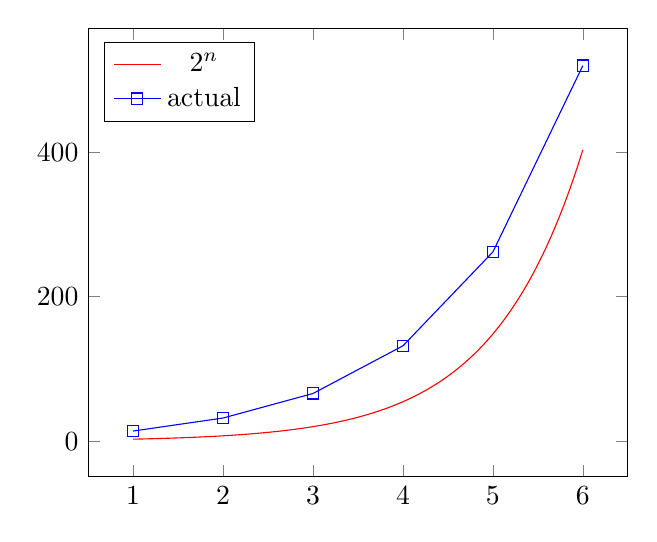
\begin{tikzpicture}
    \begin{axis}[
        legend pos= north west
        ]
       \addplot[
            domain=1:6,
            samples=100,
            color=red
        ]{exp(x)};
        \addlegendentry{$2^n$}

        \addplot[
            color=blue,
            mark=square
        ]
        coordinates {
(1,14)  (2,32)  (3,66) (4,132) (5,262) (6,520)
        };
        \addlegendentry{actual}

        %\addplot[
            %color=green,
            %mark=triangle
        %]
        %coordinates {
%(1,47)  (2,78) (3,128) (4,211) (5,347) (6,570)
        %};
        %\addlegendentry{fitted}

   \end{axis} 
\end{tikzpicture}
    \caption{Plot of type variables in Hindley-Milner type systems}
    \label{fig:expplot}
\end{figure}
\section{Higher level type systems}
The Hindley-Milner type system can only express relatively simple programs which robs algorithmic elegance in respect to other type systems.
One domain of programs that Hindley-Milner cannot express are those that rely on \textit{parametric polymorphism}.
Parametric polymorphism (or rank-n types) deals with letting abstractions have polymorphic parameters such that a type can be quantified within another type, having its depth bounded by n (rank-\textbf{n}).
For instance \autoref{lst:rankn} is not typable in Hindley-Milner since its type is \texttt{$\forall\tau$.($\forall\gamma$.$\gamma \rightarrow$ Int) $\rightarrow \tau \rightarrow$ Int}.
\begin{lstlisting}[language=ML,caption={Program that requires parametric polymorphism},label={lst:rankn},mathescape=true]
fun f makeNum a =
    ((makeNum a) + (makeNum 0)) + (makeNum (0 == 2))
\end{lstlisting}
More generally, any type which is quantified on the left side of $\rightarrow$ cannot be moved out thus increases the rank.

Even languages which are typed and inferred by Hindley-Milner like Ocaml have introduced kinds through modules to allow higher-kinded types.
Hindley-Milner is in fact a restricted version of another more general type system called \textit{System F} (and System F\underline{$\omega$}).
The Hindley-Milner type system introduces abstractions as monomorphic types whereas a system named System F allows any type to be polymorphic.
It turns out that allowing higher rank polymorphism makes type inference (type construction in older literature) \textit{undecidable}~\cite{wells1999typability}.
\begin{remark}
    Formal type systems are in the form of deductive systems, in which one can prove \textit{decidability} among other properties.
    Decidability in deductive systems is a property which expresses whether a system can be decided by an algorithm (which relates to the encoding of algorithms on theoretic computers).
    If and only if every valid formula (type) in the deductive system (type system) can have its correctness decided algorithmically.
\end{remark}

Another variant of type system is \textit{System F\underline{$\omega$}}.
System F\underline{$\omega$} introduces another feature (System F\underline{$\omega$} is different to System F, it is not an extension) called type constructors.
It is uncommon to use System F\underline{$\omega$} on its own since it only allows type constructors of monomorphic types (System F introduces polymorphism), which does not yield much expressiveness since only specific types such as \texttt{Int $\rightarrow$ List Int} would be expressible.
Throughout this chapter, type constructors have already been introduced in such a way that they can occur in Hindley-Milner though algebraic data types such as \texttt{$\forall$a.a $\rightarrow$ List a}.
Very commonly moderately generalized types need both the higher rank polymorphism implied by System F and the type constructors implied by System F\underline{$\omega$}.

Hindley-Milner can only take advantage of System F\underline{$\omega$} for rank 1 types which significantly constrains the generalization level.
A more expressive version of Hindley-Milner is System F$\omega$ which in fact, is the basis for the type system of Haskell, which is very expressive.
\begin{remark}
    Haskell has introduced some additional tweaks to System F$\omega$ to avoid the decidability problem among others.
\end{remark}

In more expressive functional programming language type systems it has become increasingly popular abstract over implementations by introducing concepts from \textit{category theory}.
Naturally many abstractions of category theory require rank-2 polymorphism.
More generally the larger the level of polymorphism allowed the larger the possible abstraction level becomes.
For instance a general purpose \textit{functor} is implementable and usable with rank-2 polymorphism while a natural transformation between kinds becomes a matter of rank-3 polymorphism.
\begin{remark}
    A functor is a mapping between two categories, which for instance can be a functor for lists which provides the algebra \texttt{$\forall$a.$\forall$b.List a $\rightarrow$ List b}.
\end{remark}
\noindent To generalize functor one must be able to express the type \texttt{$\forall\tau$.($\forall$a.a $\rightarrow$ $\tau$a) $\rightarrow$ ($\forall$b.b $\rightarrow \tau$b)} such that applying \texttt{List} effectively partially applies the type and reduces the rank.

\begin{figure}
    \centering
    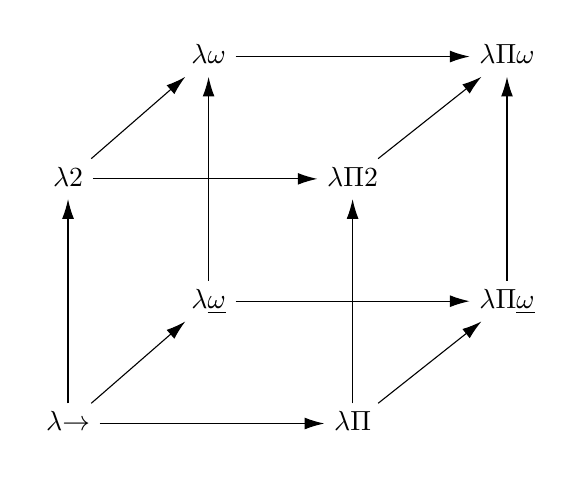
\begin{tikzpicture}
        \matrix (m) [matrix of math nodes,
        row sep=3em, column sep=3em,
        text height=1.5ex,
        text depth=0.25ex]{
                    & \lambda\omega             &              & \lambda\Pi\omega             \\
        \lambda 2   &                           & \lambda\Pi 2                                \\
                    & \lambda\underline{\omega} &              & \lambda\Pi\underline{\omega} \\
        \lambda{\to}&                           & \lambda\Pi  \\
        };
        \path[-{Latex[length=2.5mm, width=1.5mm]}]
        (m-1-2) edge (m-1-4)
        (m-2-1) edge (m-2-3)
                edge (m-1-2)
        (m-3-2) edge (m-1-2)
                edge (m-3-4)
        (m-4-1) edge (m-2-1)
                edge (m-3-2)
                edge (m-4-3)
        (m-3-4) edge (m-1-4)
        (m-2-3) edge (m-1-4)
        (m-4-3) edge (m-3-4)
                edge (m-2-3);
    \end{tikzpicture}
    \captionsetup{singlelinecheck=off}
    \caption[nothing, items]{
        \begin{itemize}
            \item$\lambda\rightarrow$ is the simply typed lambda calculus without polymorphism.
            \item$\lambda\underline{\omega}$ is System F\underline{$\omega$}.
            \item$\lambda 2$ is System F.
            \item$\lambda\omega$ is System F$\omega$.
            \item$\Pi$ introduces \textit{dependent types} which is beyond the scope of this thesis.
        \end{itemize}
    }
    \label{lambdacube}
\end{figure}
\autoref{lambdacube} shows the \textit{lambda cube}, introduced in \cite{barendregt1991introduction} which encapsulates the family of formal type systems.
Complicated type systems such as the \textit{calculus of constructions} ($\lambda\Pi\underline{\omega}$) is used in proof assistants.



\end{document}


\end{document}


\chapter{Program evaluation}
The untyped lambda calculus may provide a simple interface for programming but does not pair very well with the modern computer.
\textit{Interpreting} is a common technique for evaluating the untyped lambda calculus.
An interpreter is an execution engine usually implemented in a more low-level language.
%Formally an interpreter for the untyped lambda calculus is a confluent catamorphism on a program, which sounds like \textit{abstract nonsense}, so let us delve into the details.

\section{Evaluation strategies}
\label{sec:es}
When evaluating the untyped lambda calculus one has to choose an evaluation strategy.
The choice of evaluation strategy has a large impact on aspects such as complexity guarantees.
Such strategies are \textit{call by value}, \textit{call by name} and \textit{call by need}.
Call by value is most often the simplest and most natural way of assuming program execution.
\begin{lstlisting}[language=ML,caption={Program that doubles values},label={lst:callbyvalue},mathescape=true]
fun main =
  fun double x = x + x;
  let a = double 10;
  double 10;
\end{lstlisting}
By the call by value semantics, \autoref{lst:callbyvalue} eagerly evaluates every expression.
Clearly the variable \texttt{a} is never used but under the call by value semantics everything is eagerly evaluated.
Every expression is evaluated in logical order in the call by value evaluation strategy.
\newline
\begin{minipage}{\textwidth}
\begin{lstlisting}[language=ML,caption={Implementation of call by name},label={lst:callbyname},mathescape=true]
fun main = 
  fun suspend x unit = x;
  fun force x = x 0;
  let value = suspend 10;
  fun double x = 
      fun susExpensiveOp unit = 
          (force x) + (force x);
      susExpensiveOp;
  let a = double value;
  force (double value);
\end{lstlisting}
\end{minipage}
The call by name semantics however does only evaluate expressions once they are needed.
By the call by name semantics \texttt{a} is never evaluated since it is never used.
In \autoref{lst:callbyname} call by name has been implemented by the use of various functions such as the two constant functions \texttt{suspend} and \texttt{force}.
\texttt{susExpensiveOp} ensures that the forcing (evaluation) of \texttt{x} never occurs until the caller of \texttt{double} forces the result.
By the aforementioned semantics of call by name in the context of the program in \autoref{lst:callbyname} \texttt{a} is never forced thus the computation is never performed.
The implementation of call by name can become quite troublesome and therefore in most cases is a part of the native execution environment which will be discussed in \autoref{tbd}.

The call by need strategy introduces \textit{lazy evaluation} semantics which is the same as call by name with one extra detail named \textit{sharing}.
In \autoref{lst:callbyname} \texttt{force x} is computed twice which may be an expensive operation.
Under call by need all results are saved for later use similar to techniques such as dynamic programming.
\begin{figure}
    \centering
    \begin{subfigure}[b]{0.33\textwidth}
        \centering
        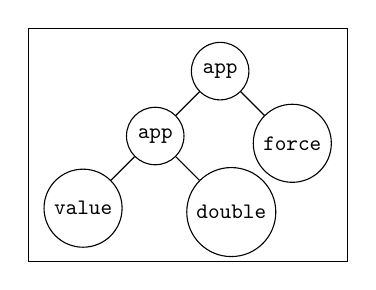
\begin{tikzpicture}[ scale=0.8, every node/.style={scale=0.8}, node distance = 0.3cm and 0.3cm]
                \node[circle, draw=black] (app1) {\texttt{app}};
                    \node[circle, draw=black, below right = of app1] (force) {\texttt{force}};
                    \path[-] (app1) edge node[left] {} (force);

                    \node[circle, draw=black, below left = of app1] (app2) {\texttt{app}};
                    \path[-] (app1) edge node[left] {} (app2);
                        \node[circle, draw=black, below left = of app2] (value) {\texttt{value}};
                        \path[-] (app2) edge node[left] {} (value);
                        \node[circle, draw=black, below right = of app2] (double) {\texttt{double}};
                        \path[-] (app2) edge node[left] {} (double);

                \node[draw,scale=1.3,fill=none,rectangle,fit=(app1)(value)(force)](fstB){};
        \end{tikzpicture}
        \caption{The last expression of the program.}
        \label{sub:eval:main}
    \end{subfigure}
    \begin{subfigure}[b]{0.66\textwidth}
        \centering
        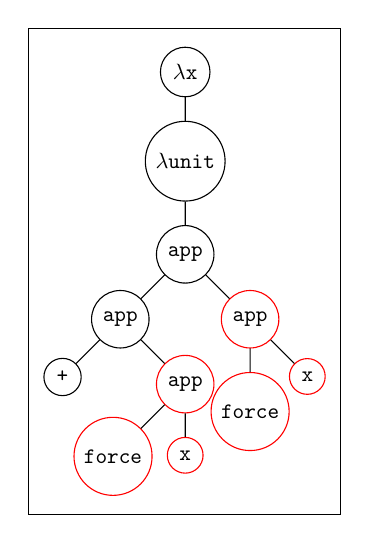
\begin{tikzpicture}[ scale=0.8, every node/.style={scale=0.8}, node distance = 0.3cm and 0.3cm]
                \node[circle, draw=black] (lamx) {\texttt{$\lambda$x}};
                    \node[circle, draw=black, below = of lamx] (lamu) {\texttt{$\lambda$unit}};
                    \path[-] (lamx) edge node[left] {} (lamu);
                        \node[circle, draw=black, below = of lamu] (app1) {\texttt{app}};
                        \path[-] (lamu) edge node[left] {} (app1);
                            \node[circle, draw=red, below right = of app1] (app2) {\texttt{app}};
                            \path[-] (app1) edge node[left] {} (app2);
                                \node[circle, draw=red, below right = of app2] (x1) {\texttt{x}};
                                \path[-] (app2) edge node[left] {} (x1);
                                \node[circle, draw=red, below = of app2] (force1) {\texttt{force}};
                                \path[-] (app2) edge node[left] {} (force1);

                            \node[circle, draw=black, below left = of app1] (app4) {\texttt{app}};
                            \path[-] (app1) edge node[left] {} (app4);
                                \node[circle, draw=black, below left = of app4] (add) {\texttt{+}};
                                \path[-] (app4) edge node[left] {} (add);

                                \node[circle, draw=red, below right = of app4] (app3) {\texttt{app}};
                                \path[-] (app4) edge node[left] {} (app3);
                                    \node[circle, draw=red, below = of app3] (x2) {\texttt{x}};
                                    \path[-] (app3) edge node[left] {} (x2);
                                    \node[circle, draw=red, below left = of app3] (force2) {\texttt{force}};
                                    \path[-] (app3) edge node[left] {} (force2);
                \node[draw,scale=1.3,fill=none,rectangle,fit=(lamx)(force2)(x1)(add)](fstB){};
        \end{tikzpicture}
    %\begin{tikzpicture}
        %\node[circle, draw=black] (lamx) {$\lambda \texttt{x}$};

        %\node[circle, draw=black, below = of lamx] (lamunit) {$\lambda \texttt{unit}$};

        %\node[circle, draw=black, below = of lamunit] (addition) {$+$};

        %\node[circle, draw=black, below left = of addition] (force1) {\texttt{force}};
        %\node[circle, draw=black, below = of force1] (x1) {\texttt{x}};
        
        %\node[circle, draw=black, below right = of addition] (force2) {\texttt{force}};
        %\node[circle, draw=black, below = of force2] (x2) {\texttt{x}};

        %\path[->] (lamx) edge node[left] {} (lamunit);
        %\path[->] (lamunit) edge node[left] {} (addition);

        %\path[->] (addition) edge node[left] {} (force1);
        %\path[->] (addition) edge node[left] {} (force2);

        %\path[->] (force1) edge node[left] {} (x1);
        %\path[->] (force2) edge node[left] {} (x2);
    %\end{tikzpicture}
        \caption{The expression tree for \texttt{double}}
        \label{sub:eval:double}
    \end{subfigure}
    \caption{}
    \label{fig:evalexpr}
\end{figure}
To understand this better observe the expression tree for \autoref{lst:callbyname} in \autoref{fig:evalexpr}.
Clearly the two red subtrees in \autoref{sub:eval:double} are identical thus they may be memoized such that the forcing of \texttt{x} only occurs once.
More generally if the execution environment supports lazy evaluation, once an expression has been forced it is remembered.

\section{Runtime environments}
Now that the untyped lambda calculus has been introduced, implemented and validated efficiently the question of execution naturally follows.
There exists many different well understood strategies to implement an execution environment for the untyped lambda calculus.
Naively it may seem straightforward to evaluate the untyped lambda calculus mechanically by $\beta$-reductions, but doing so brings upon some problems when implementing an interpreter.
%When applying the term $f x$ in $\lambda f . \lambda x . f x$ such that $f[? := x]$ where $?$ is the parameter name of $f$ it should become clear why a naive strategy is not enough since the parameters of $f$ are anonymous.



\section{Combinator reducers}
\label{sec:comb}
One of the most prominent techniques for evaluating functional programs is that of \textit{combinator graphs reductions}.
Formally a combinator is a function that has no free variables which is convenient since the problem of figuring out closures and parameter substitutions in applications never arises.
\begin{align}
    x \label{eq:comb:x}\\
    F \label{eq:comb:F}\\
    Y E \label{eq:comb:app}
\end{align}
There are three types of terms in combinator logic; the variable much like the lambda calculus (\autoref{eq:comb:x}), application (\autoref{eq:comb:app}) and the combinator (\autoref{eq:comb:F}).
The SKI calculus is a very simple set of combinators which are powerful enough to be turing complete and translate to and from the lambda calculus.
In SKI $F ::= S \,\,|\,\, K \,\,|\,\, I$ where the equivalent lambda calculus combinators for $S = \lambda x . \lambda y . \lambda z . x z (y z)$, $K = \lambda x . \lambda y . x$ and $I = \lambda x . x$.
Evaluating an SKI program is a straightforward reduction where $F'_F$ denotes combinator $F'$ has been partially applied with combinator $F$.
\begin{exmp}
    \begin{align}
        &SKSI\\
        = &KI(SI)\tag*{}\\
        = &K_I(SI)\tag*{}\\
        = &I\tag*{}
    \end{align}
\end{exmp}

The algorithm for converting a lambda calculus program into a SKI combinator program is a straightforward mechanical one.
The evaluation context is always an abstraction $\lambda x . E$.
\begin{pcases}
    \pcase{$E = x$ then rewrite $\lambda x . E$ to $I$.}
    \pcase{$E = y$ where $y \neq x$ and $y$ is a variable then rewrite $\lambda x . y$ to $Ky$.}
    \pcase{$E = Y E'$ then rewrite $\lambda x . Y E'$ to $S(\lambda x . Y)(\lambda x . E')$ since applying some $y$ to $\lambda x . Y E'$ must lambda lift $y$ as a parameter named $x$ to both $Y$ and $E'$ such that the lifted expression becomes $((\lambda x . Y)y)((\lambda x . E')y) = S(\lambda x . Y)(\lambda x . E')y$.
    Then recurse in both branches.
    }
    \pcase{$E = \lambda x . E'$ then first rewrite $E'$ with the appropriate cases recursively such that $E'$ becomes either $x$, $y$ or $Y E$ such that Case 1, 2 or 3 can be applied.}
\end{pcases}
The termination of the rewriting to SKI is guaranteed since abstractions are always eliminated and the algorithm never introduce any additional abstractions.
When translating the untyped lambda calculus to SKI the ''magic`` variable names $\sigma, \kappa$ and $\iota$ are used as placeholder functions for the SKI combinators since the translation requires a lambda calculus form.
When the translation has been completed then replace $\sigma \mapsto S, \kappa \mapsto K, \iota \mapsto I$.
\subsection{Combinator translation growth}
Before proving that the SKI translation algorithm produces a program of larger size the notion of size must be established.
Size in terms of lambda calculus are the number of lambda terms (\autoref{lc:lang:abs}, \autoref{lc:lang:var} and \autoref{lc:lang:app}) that make up a program.
For instance $\lambda x . x$ has a size of two since it is composed of an abstraction and a variable term.
The size of an SKI combinator program is in terms of the number of combinators.
\begin{lemma}
    There exists a family of lambda calculus programs of size $n$ which are translated into SKI-expressions of size $\Omega(n^2)$.
\end{lemma}
\begin{proof}
\begin{pcases}
    \pcase{\label{eval:case:1} Rewriting $\lambda x . x$ to $I$ is a reduction of one.}
    \pcase{\label{eval:case:2} Rewriting $\lambda x . y$ to $Ky$ is equivalent in terms of size.}
    \pcase{Rewriting $\lambda x . YE$ to $S(\lambda x . Y)(\lambda x . E)$ is the interesting case.
        To induce the worst case size \autoref{eval:case:1} must be avoided.
        If $x \notin \textit{Free}(Y)$ and $x \notin \textit{Free}(E)$ then for every non-recursive term in $Y$ and $E$ \autoref{eval:case:2} is the only applicable rewrite rule which means that an at least equal size is guaranteed.
        Furthermore observe that by introducing unused parameters one can add one $K$ term to \textit{every} non-recursive case.
        Observe the instance $\lambda f_1 . \lambda f_2 . \lambda f_3 . (f_1 f_1 f_1)$ where the two unused parameters are used to add $K$ terms to all non-recursive cases in \autoref{eq:eval:red2} such that the amount of extra K terms minus the I becomes $\text{variable\_references} * (\text{unused\_abstractions} - 1) = 3*(3-1)$:
        \begin{gather}
            S(S(KKI)(KKI))(KKI)\label{eq:eval:red2}
        \end{gather}
        Now let the number of variable references be $n$ and the unused abstractions also be $n$ clearly $\Omega(n * (n - 1)) = \Omega(n^2)$
    }
    \pcase{Rewriting $\lambda x . E'$ is not a translation rule so the cost is based on what $E'$ becomes.}
\end{pcases}
    \vspace*{0.5cm}
Notice that the applications $f_1 f_1 \dots f_1$ can in fact be changed to $f_1 f_2 \dots f_n$ since for every $f_k$ where $0 < k \leq n$ there are $n - 1$ parameters that induce a K combinator.
Let $P_n$ be family of programs with $n$ abstractions and $n$ applications.
$\lambda f_1 . \lambda f_2 . \lambda f_3 . (f_1 f_1 f_1) \in P_3$ and in fact for any $p$ where $\forall n \in \mathbb{Z}^+$ and $p \in P_n$, $p$ translates into SKI-expressions of size $\Omega(n^2)$.
\end{proof}
\begin{exmp}
    Observe the size of \autoref{eq:eval:comp1} in comparison to \autoref{eq:evaltime}.
\begin{align}
    &\lambda f_1 . \lambda f_2 . f_1 f_2 \label{eq:eval:comp1}\\
    =&\lambda f_1 . \sigma(\lambda f_2 . f_1)(\lambda f_2 . f_2) \tag*{} \\
    =&\lambda f_1 . (\sigma(\kappa f_1))(\iota) \tag*{} \\
    =&\sigma (\lambda f_1 . \sigma (\kappa f_1)) (\lambda f_1 . \iota) \tag*{} \\
    =&\sigma (\sigma (\lambda f_1 . \sigma) (\lambda f_1 . \kappa f_1)) (\kappa \iota) \tag*{} \\
    =&\sigma (\sigma (\kappa \sigma) (\sigma (\lambda f_1 . \kappa) (\lambda f_1 . f_1))) (\kappa \iota) \tag*{} \\
    =&\sigma (\sigma (\kappa \sigma) (\sigma (\kappa \kappa) (\iota))) (\kappa \iota) \tag*{} \\
    =&S (S (K S) (S (K K) (I))) (K I) \tag*{}
\end{align}
\end{exmp}
It should become clear that many programs suffer from this consequence such as \texttt{let add = ($\lambda$x.$\lambda$y.(+ x) y)} $\in P_2$ where the program is written in prefix notation.
Translating the lambda calculus into the SKI-expressions does indeed increase the size significantly but does not warrant a write off entirely.
More advanced techniques exist to translate the lambda calculus to linearly sized SKI-expressions with the introduction of more complicated combinators~\cite{kiselyov2018lambda}.


\section{Reduction strategies}
Reductions in the context of the lambda calculus are a small set of well-defined rules for rewriting such that a program is proved or evaluated.
The techniques required to correctly prove and evaluate a program are a bit more complicated than the SKI calculus but are rewarding in flexibility and performance.
Throughout this section we will explore what difficulties lie within proving and evaluating the untyped lambda calculus via reduction strategies.
The first section will interest itself with the semantics of proving the untyped lambda calculus, whilst the second will implement a machine capable of evaluating a result.

\subsection{Symbols and notation}
The following sections will have many variables with different meaning, therefore symbols are constrained to certain types of values as described in \autoref{eq:redstrat:sym}.
\begin{align}
  \texttt{x, y, z, f, v, $\gamma$ }&\texttt{:= Var}\label{eq:redstrat:sym}\\
  \texttt{e, p, l, o }&\texttt{:= Exp}\tag*{}\\
  \texttt{$\Gamma$, $\Sigma$, $\Theta$, S }&\texttt{:= Heap}\tag*{}\\
  \texttt{E, $\mathcal{E}$ }&\texttt{:= Environment}\tag*{}
\end{align}
\texttt{Exp} is any expression, expressible in both untyped lambda calculus and future extensions.


\subsection{The abstract evaluation model}
The environment is a set of substitutions, that is, a set of variable names to their value denoted \texttt{\{x $\mapsto$ $\lambda$y.y\}} meaning ``the value of variable \texttt{x} is \texttt{$\lambda$y.y}''.
\begin{remark}
  In the section regarding the semantics of reduction strategies, environments will exist as singleton sets, named \textit{substitutions}.
\end{remark}
%Substitutions mappings can be combined $S \cup \Sigma$, if a variable name occurs in both $S$ and $\Sigma$ then the variable in the rightmost mapping is chosen ($\Sigma$).
\begin{align}
  \texttt{\{x $\mapsto$ y\}x = y}\label{eq:subsem}
\end{align}
Substitutions are performed like shown in \autoref{eq:subsem}, which states ``x is substituted by y''.
%In $(\lambda f . \lambda x . \lambda y. \texttt{ let } a = f x \texttt{ in } a + y)(\lambda y . y) \,\, 10 \,\, 20$ when evaluating $f x$ where the substitution are $[f \mapsto \lambda y . y, x \mapsto 10, y \mapsto 20]$ there must be taken great care that $x$ is mapped to $y$ in $\lambda y . y$.

Evaluation strategies (\autoref{sec:es}) are a core part of the reduction strategy since the choice of evaluation strategy determines the order in which terms are evaluated.
%A \textit{redex} is a reducible expression in the context of some set of reduction rules.
%The two interesting evaluation orders are \textit{applicative order} and \textit{normal order}~\cite{sestoft2002demonstrating}.
%The most interesting evaluation order is 
%Applicative order specifies that the parameters of some application should always be evaluated first, e.g. call by value.
%Normal order specifies that the leftmost outermost term should be evaluated first which yields the call by name strategy.
The order of evaluation decides the evaluation strategy and also the final form of expressions~\cite{sestoft2002demonstrating}.
Before delving into more complicated evaluation strategies such as call by need, call by name will be considered.

A reduction strategy would involve substituting variables, once they are applied.
When evaluating a term such as \texttt{($\lambda$x.x) y}, \texttt{x} must be substituted by \texttt{y} such that the expression then becomes \texttt{x} with the substitution \texttt{\{x $\mapsto$ y\}} and finally becomes \texttt{y} after the substitution has occurred.
\begin{figure}[ht]
    \begin{mdframed}[style=bigbox]
        \vspace*{0.49cm}
        \begin{subfigure}[b]{0.48\textwidth}
            \begin{prooftree}
                \AxiomC{}
                \RightLabel{Abs}
                \UnaryInfC{\texttt{($\lambda$x.e) $\rightarrow$ ($\lambda$x.e)}}
            \end{prooftree}   
            \caption{}
            \label{eq:simpleabs}
        \end{subfigure}
        \begin{subfigure}[b]{0.48\textwidth}
            \vspace*{0.4cm}
            \begin{prooftree}
                \AxiomC{}
                %\AxiomC{$S \alpha x \not\equiv \alpha x$}
                \RightLabel{Var}
                \UnaryInfC{\texttt{x $\rightarrow$ x}}
            \end{prooftree}   
            \caption{}
            \label{eq:simplevar}
        \end{subfigure}
        \begin{subfigure}[b]{1\textwidth}
            \vspace*{0.4cm}
              \begin{prooftree}
                \AxiomC{\texttt{\{x $\mapsto$ e\} p $\rightarrow$ l}}
                  \RightLabel{Let}
                  \UnaryInfC{\texttt{let x = e in p $\rightarrow$ l}}
              \end{prooftree}   
          \caption{}
          \label{fig:simplelet}
        \end{subfigure}
        \begin{subfigure}[b]{1\textwidth}
            \vspace*{0.4cm}
              \begin{prooftree}
                \AxiomC{\texttt{l $\rightarrow$ ($\lambda$x.e)}}
                \AxiomC{\texttt{\{x $\mapsto$ p\} e $\rightarrow$ o}}
                  \RightLabel{App}
                  \BinaryInfC{\texttt{l p $\rightarrow$ o}}
              \end{prooftree}   
          \caption{A simple application rule}
          \label{fig:simpleapp}
        \end{subfigure}
    \end{mdframed}
    \caption{Simple call by name lambda calculus}
    \label{fig:scbn}
\end{figure}
The rules in \autoref{fig:scbn} display a simple set of rules for proving call by name lambda calculus programs.
\begin{itemize}
\item The Abs and Var rules (\autoref{eq:simpleabs} and \autoref{eq:simplevar}) are rules which act as terminal cases of a proof.
      Abs and Var both state that if either of them occur then the expression must be an axiom by their identity.
\item The App rule (\autoref{fig:simpleapp}) states that ``\texttt{l p} can be proved to evaluate to \texttt{o} if \texttt{l} can be proved to be \texttt{($\lambda$x.e)} and \texttt{e} can be proved to evaluate to \texttt{o}, where \texttt{x} has been replaced by \texttt{p} in \texttt{e}''.
\item The Let rule has the same function as the App rule, but will have an important role in a more refined version of the semantics.
\end{itemize}
We must introduce rules for how substitutions should act upon encountering lambda calculus terms (\autoref{eq:subsem}).
\begin{align}
  &\texttt{\{x $\mapsto$ e\}x = e} \label{eq:subsem}\\
  &\texttt{\{x $\mapsto$ e\}p = p}  \tag*{}\\
  &\texttt{E(l p) = (El)(Ep)} \tag*{}\\
  &\texttt{E($\lambda$x.e) = ($\lambda$x.Ee) } \label{eq:subsemrem}%\\
\end{align}

\subsubsection{Ambiguous programs}
\begin{align}
  \texttt{($\lambda$x.($\lambda$x.x) 0) 1} \label{eq:ambgprog}
\end{align}
Proving \autoref{eq:ambgprog} under the rules in \autoref{eq:subsem} yields a case for more thorough substitution rules.
By inspection one can determine that a simple program like \autoref{eq:ambgprog} yields the symbol \texttt{0}, but alas this is not the case.
The first step to prove \autoref{eq:ambgprog} is to apply through the App rule, which prompts the application of the Abs rule on the left side for \texttt{f}, such that the expression to prove now becomes the lambda abstraction with \texttt{x} replaced by \texttt{1} (\autoref{eq:ambgprog2}).
\begin{align}
  \texttt{($\lambda$x.1) 0} \label{eq:ambgprog2}
\end{align}
Clearly \autoref{eq:ambgprog2} changed the meaning of the program.
If we continue the proof which states that the program in \autoref{eq:ambgprog2} should evaluate to the symbol \texttt{0}, we would not be in luck.
Clearly this system is not sound, thus requires some further refinement.
%\begin{figure}
%\begin{lstlisting}[language=ML,caption={Program with variable ambiguity},label={lst:varambg},mathescape=true]
%fun f x =
  %fun g x = x;
  %g (x + x);
%f 2;
%\end{lstlisting}
%\end{figure}
%Evaluating \autoref{lst:varambg} under the rules in \autoref{eq:subsem} yields a case for more thorough substitution rules.
%Using the App rule (\autoref{fig:simpleapp}) and applying substitutions as defined in (\autoref{eq:subsem}), yields the program in \autoref{lst:varambg2}.
%\begin{lstlisting}[language=ML,caption={Program with variable ambiguity after one reduction pass},label={lst:varambg2},mathescape=true]
%fun g x = 2;
%g (2 + 2);
%\end{lstlisting}
%Which eventually evaluates to \texttt{2}, which clearly is not the intended result.
Removing the rule \autoref{eq:subsemrem} and adding the two rules in \autoref{eq:subsemfixed} solves this type.
\begin{align}
  &\texttt{E($\lambda$x.e) = ($\lambda$x.Ee)} & \texttt{(x $\mapsto$ p) $\notin$ S} \label{eq:subsemfixed}\\
  &\texttt{E($\lambda$x.e) = ($\lambda$x.(E$\backslash$\{x $\mapsto$ p\})e)} & \texttt{(x $\mapsto$ p) $\in$ S} \tag*{}
\end{align}
This is a simple instance of variable ambiguity, a more problematic variant exists which goes by the name of variable capture.
This evaluation model is indeed powerful enough to evaluate \textbf{most} call by name lambda calculus programs.
\begin{exmp}
  With the aforementioned rules, programs can now be proved.
  Note that the Substitution rule in \autoref{fig:rules:exmp:sol} is simply the substitution semantics from \autoref{eq:subsemfixed} made clearer.
  Let the program in \autoref{eq:exmp:subrules}, where \texttt{0} is a symbol of any type, be subject to the rules in \autoref{fig:scbn}, which solves to \autoref{fig:rules:exmp:sol}.
  \begin{align}
    \texttt{(($\lambda$f.$\lambda$x.f x) ($\lambda$x.x)) 0}\label{eq:exmp:subrules}
  \end{align}
  \begin{figure}[ht]
    \begin{mdframed}
        \vspace*{0.49cm}
      \begin{subfigure}[b]{1\textwidth}
        \begin{prooftree}
    \AxiomC{}
    \LeftLabel{Abs}
  \UnaryInfC{\texttt{($\lambda$x.($\lambda$x.x) x) $\rightarrow$ ($\lambda$x.($\lambda$x.x) x)}}
\LeftLabel{Substitution}
\UnaryInfC{\texttt{\{f $\mapsto$ ($\lambda$x.x)\}($\lambda$x.f x) $\rightarrow$ ($\lambda$x.($\lambda$x.x) x)}}
        \end{prooftree}
        \caption{}
        \label{fig:rules:exmp:left:right}
      \end{subfigure}
        \vspace*{0.49cm}
      \begin{subfigure}[b]{1\textwidth}
        \begin{prooftree}
    \AxiomC{}
  \LeftLabel{Abs}
  \UnaryInfC{\texttt{($\lambda$f.$\lambda$x.f x) $\rightarrow$ ($\lambda$f.$\lambda$x.f x)}}
  \AxiomC{\autoref{fig:rules:exmp:left:right}}
\LeftLabel{App}
\BinaryInfC{\texttt{($\lambda$f.$\lambda$x.f x) ($\lambda$x.x) $\rightarrow$ ($\lambda$x.($\lambda$x.x) x)}}
        \end{prooftree}
        \caption{}
        \label{fig:rules:exmp:left}
      \end{subfigure}
        \vspace*{0.49cm}
      \begin{subfigure}[b]{1\textwidth}
        \begin{prooftree}
      \AxiomC{}
    \LeftLabel{Abs}
    \UnaryInfC{\texttt{($\lambda$x.x) $\rightarrow$ ($\lambda$x.x)}}
        \AxiomC{}
      \RightLabel{Var}
      \UnaryInfC{\texttt{0 $\rightarrow$ 0}}
    \RightLabel{Substitution}
    \UnaryInfC{\texttt{\{x $\mapsto$ 0\}x $\rightarrow$ 0}}
  \RightLabel{App}
  \BinaryInfC{\texttt{($\lambda$x.x) 0 $\rightarrow$ 0}}
\RightLabel{Substitution}
\UnaryInfC{\texttt{\{x $\mapsto$ 0\}($\lambda$x.x) x $\rightarrow$ 0}}
        \end{prooftree}
        \caption{}
        \label{fig:rules:exmp:right}
      \end{subfigure}
        \vspace*{0.49cm}
      \begin{subfigure}[b]{1\textwidth}
        \begin{prooftree}
  \AxiomC{\autoref{fig:rules:exmp:left}}
  \AxiomC{\autoref{fig:rules:exmp:right}}
\LeftLabel{App}
\BinaryInfC{\texttt{(($\lambda$f.$\lambda$x.f x) ($\lambda$x.x)) 0 $\rightarrow$ 0}}
        \end{prooftree}
      \end{subfigure}
    \end{mdframed}
    \caption{}
    \label{fig:rules:exmp:sol}
  \end{figure}
\end{exmp}

Variable capture is the basis for some practical difficulties when designing evaluation rules for the untyped lambda calculus.
Consider the following sub-program \texttt{($\lambda$x.y) g} with the following ongoing substitutions \texttt{\{x $\mapsto$ z, y $\mapsto$ x, $\dots$\}}, which contains \texttt{y} as a closure.
Substituting by the rules outlined in \autoref{eq:subsemfixed} yields \texttt{($\lambda$x.x) g} which is clearly invalid.
The invalid program result is a product of variable capture.
%The program before substitution and after should be \textit{$\alpha$-equivalent}, which they are not.
%The two program states becomes ambiguous by the ambiguity of multiple variables by the same name.
To solve ambiguity between variables with the same name, one can perform an \textit{$\alpha$-conversion}.
\begin{remark}
  Notice that if variables are renamed before program execution, recursive functions can still suffer from ambiguity since all parameters for that function can occur multiple times.
\end{remark}
\subsubsection{$\alpha$-conversions} \label{sec:alpha}
%An $\alpha$-conversion mapping can occur as the substitution mapping, that is \texttt{\{x $\mapsto$ $\gamma_1$, y $\mapsto$ $\gamma_2$\}}; $\alpha$-conversions are philosophical constructs more than materialized mappings.
An $\alpha$-conversion is a renaming operation which does not modify the meaning of the expression.
$\alpha$-conversions can appear similar to substitutions, for instance renaming \texttt{x} to $\gamma$ appears as \texttt{\{x $\mapsto$ $\gamma$\}}.
$\alpha$-conversions guarantee what is called \textit{$\alpha$-equivalence} which is the notion of semantic equivalence.
For instance \texttt{$\lambda$x.x} is $\alpha$-equivalent with \texttt{$\lambda\gamma.\gamma$} since both expressions are semantically equivalent.
%$\alpha$-conversions solve some critical problems such as closures and recursion when evaluating the lambda calculus.
%$\alpha$-conversions should also be non-destructive but still be context aware such that when leaving an abstraction the remaining substitution mapping is a superset of the substitution mapping when entering.
%More formally if \texttt{S, e $\rightarrow$ $\Sigma$, e'} then $\{x \,\,|\,\, (x \mapsto y) \in S\} \subseteq \{x \,\,|\,\, (x \mapsto y) \in \Sigma\}$.
%\begin{lstlisting}[language=ML,caption={Recursive addition function},label={lst:recalpha},mathescape=true]
%let f = ($\lambda$f'.$\lambda$x.
    %if (x = 0) x else f' f' ((x - 1) + (x - 1))) in
%f f 10
%\end{lstlisting}
%A strong guarantee that can be made by tuning the evaluation strategy which is particularly useful for $\alpha$-conversion algorithms is that \textit{any} returned value has had \textit{every} term that it contains visited.
%An algorithm for performing $\alpha$-conversions can be implemented that picks a new variable name from any infinite domain when an abstraction has had a value applied to it and replaces future encountered variables with the new one, such an algorithm only works if the guarantee of visiting every term is made.
%The algorithm should also introduce the applied value to the substitution set through the alpha converted name.
\noindent An $\alpha$-conversion algorithm can be implemented such that when a new variable is introduced through an abstraction, a new name for the variable is given.
More formally; Let $V_1$ be the domain of variables in the program and $V_2$ be the infinite domain for variable names that satisfies $V_1 \cap V_2 = \emptyset$, such that when a new variable \texttt{x} is discovered, replace it with some $\gamma \in V_2$ and let $V_2 = V_2 \backslash \{\gamma\}$. 
Working with the previous example \texttt{\{y $\mapsto$ x\}($\lambda$x.y) g}
%For instance, let \texttt{($\lambda\gamma_1$.$\lambda\gamma_2$.if ($\gamma_2$ = 0) $\gamma_2$ else $\gamma_1$ $\gamma_1$ (($\gamma_2$ - 1) + ($\gamma_2$ - 1)))} be the $\alpha$-converted version of \texttt{f} in \autoref{lst:recalpha}.
The function \texttt{fresh} picks a fresh variable name $\gamma$ from $V_2$ and updates $V_2$ to $V_2 \backslash \{\gamma\}$.
$\alpha$-conversions will be further explored in future refinements of \autoref{fig:scbn} in the from of renaming through the Let rule.
\\

%\subsubsection{Eager substitutions}
%Instead of performing $\alpha$-conversions to ensure variable uniqueness, one can enhance the rules in \autoref{fig:scbn}.%one can leverage the ideas proposed in~\cite{launchbury1993natural} to implement laziness, lazy substitution, solve variable ambiguity and perform efficient garbage collection.
%To further refine the call by name evaluation semantics observe that substitutions are performed eagerly, that is, they \textit{break suspension}.
%To explore solutions to avoid eager substitutions, environments may be used.
%\begin{remark}
  %When considering an arbitrarily large expression under call by name (or need), there is no guarantee that the expression will ever be evaluated, that is, a suspended expression being forced.
  %Rules specify what implementations must adhere to and not anything more.
  %Regardless it still remains as an interest to not break suspension.
  %Breaking suspension may violate the philosophy behind call by name (and need).
  %A solution could involve composing a function in compile time, which replaces all instances of a variable (by \autoref{eq:subsem} and \autoref{eq:subsemfixed}) with some parameterized value.
  %Substituting expressions eagerly might compromise practical performance guarantees, even if substitution is an asymptotically constant number of operations.
  %Consider substituting an expression which contains conditional branches, one branch might be a simple expression and the other might be a very large expression, consisting of many instances of the same variable.
  %If the program never picks the large expression, why should it ever have any impact on performance.
  %For instance, in \autoref{lst:fastslow} under call by name one would expect \texttt{fastMap} to evaluate in roughly the same time as \texttt{slowMap}.
%\begin{lstlisting}[language=ML,caption={Performance considerations in substitution},label={lst:fastslow},mathescape=true]
%fun fastMap f l =
  %match l
    %| Nil -> Nil;
    %| Cons x xs -> Cons (f x) (map f xs);
  %;
%fun slowMap f l =
  %match l
    %| Nil -> Nil;
    %| Cons x xs -> 
      %if (x == 0)
        %let v = x + x + x + x + x + x; 
        %Cons (f x) (map f xs);
      %else
        %Cons (f x) (map f xs);
      %;
  %;
%\end{lstlisting}
%\end{remark}
\subsubsection{The heap}
Heaps, like environments in typing (\autoref{eq:env}), define what ``state'' is required to evaluate some expression.
A heap contains mappings from variables to expressions, much like the environment which performs substitutions, except it acts like a store.
Heaps are a requirement for call by need semantics.
A simple modification to the rules in \autoref{fig:rules:env}, introduces a heap which states that that the semantics must bring a heap along. 
\begin{figure}[ht]
    \begin{mdframed}[style=bigbox]
        \vspace*{0.49cm}
        \begin{subfigure}[b]{0.49\textwidth}
            \begin{prooftree}
                \AxiomC{}
                \RightLabel{Abs}
                \UnaryInfC{\texttt{$\Gamma$, ($\lambda$x.e) $\rightarrow$ $\Gamma$, ($\lambda$x.e)}}
            \end{prooftree}   
            \caption{}
          \label{fig:rules:env:abs}
        \end{subfigure}
        \begin{subfigure}[b]{0.49\textwidth}
            \vspace*{0.4cm}
              \begin{prooftree}
                \AxiomC{\texttt{$\Gamma$ $\cup$ \{x $\mapsto$ e\}, p $\rightarrow$ $\Theta$, l}}
                  \RightLabel{Let}
                  \UnaryInfC{\texttt{$\Gamma$, let x = e in p $\rightarrow$ $\Theta$, l}}
              \end{prooftree}   
          \caption{}
          \label{fig:rules:env:let}
        \end{subfigure}
        \begin{subfigure}[b]{1\textwidth}
          \vspace*{0.4cm}
          \begin{prooftree}
            \AxiomC{\texttt{$\Gamma$, l $\rightarrow$ $\Theta$, ($\lambda$x.e)}}
            \AxiomC{\texttt{$\Theta$, \{x $\mapsto$ p\}e $\rightarrow$ $\Sigma$, o}}
              \RightLabel{App}
              \BinaryInfC{\texttt{$\Gamma$, l p $\rightarrow$ $\Sigma$, o}}
          \end{prooftree}   
          \caption{}
          \label{fig:rules:env:app}
        \end{subfigure}
        \begin{subfigure}[b]{1\textwidth}
          \vspace*{0.4cm}
            \begin{prooftree}
                \AxiomC{\texttt{$\Gamma$, e $\rightarrow$ $\Theta$, p}}
                \RightLabel{Var}
                \UnaryInfC{\texttt{$\Gamma$ $\cup$ \{x $\mapsto$ e\}, x $\rightarrow$ $\Theta$ $\cup$ \{x $\mapsto$ e\}, p}}
            \end{prooftree}   
            \caption{}
          \label{fig:rules:env:var}
        \end{subfigure}
    \end{mdframed}
    \caption{Call by name lambda calculus with environments}
    \label{fig:rules:env}
\end{figure}
The rules in \autoref{fig:rules:env} are quite different from the rules in \autoref{fig:scbn}.
\begin{itemize}
  \item Var is no longer terminal, it now inspects the heap for a replacement value for some \texttt{x}.
    Notice that Var now removes the mapping from the heap $\Gamma$ such that recursively defined expressions cannot occur.
  \item Let now has a role which is distinct from App.
    Let now introduces values to the heap, but does not induce a substitution.
  \item App remains the same by eagerly substituting, but now augmented with a heap.
  \item Abs is now augmented with a heap.
\end{itemize}
The rules in \autoref{fig:rules:env} are not any more powerful that the rules in \autoref{fig:scbn}, but are a basis for lazy evaluation.

\subsubsection{Lazy evaluation}
With the revised semantics in \autoref{fig:rules:env}, lazy evaluation can now be introduced.
The basis for sharing evaluated expressions is rooted in a labelling problem~\cite{levy1988sharing}.
Before delving into a set of rules which use a labelling technique, consider that sharing can be viewed as a dependency graph of expressions.
Let \autoref{fig:dependencygraph} be a depiction of the dependency graph of \autoref{eq:xyk} under the rules in \autoref{fig:rules:env}.
\begin{align}
  &\texttt{let k = ($\lambda$z.z) ($\lambda$f.f) in }\label{eq:xyk}\\
  &\texttt{let x = k in }\tag*{}\\
  &\texttt{let y = k in }\tag*{}\\
  &\texttt{x + y}\tag*{}
\end{align}
\begin{figure}[ht]
  \centering
  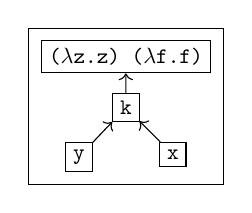
\begin{tikzpicture}[ scale=0.8, every node/.style={scale=0.8}, node distance = 0.25cm and 0.25cm]
      \node[draw=black] (e) {\texttt{($\lambda$z.z) ($\lambda$f.f)}};

          \node[draw=black, below = of e] (k) {\texttt{k}};
          \path[->] (k) edge node[left] {} (e);
            
              %\node[draw=black, below left = of k] (gamma1) {$\gamma_1$};
              %\path[->] (gamma1) edge node[left] {} (k);

              \node[draw=black, below left = of k] (y) {\texttt{y}};
              \path[->] (y) edge node[left] {} (k);

            %\node[draw=black, below right = of k] (gamma2) {$\gamma_2$};
            %\path[->] (gamma2) edge node[left] {} (k);

              \node[draw=black, below right = of k] (x) {\texttt{x}};
              \path[->] (x) edge node[left] {} (k);

          \node[draw,fill=none,scale=1.3,rectangle,fit=(e)(x)(y)](fbb){};
  \end{tikzpicture}
  \caption{Expression dependencies}
  \label{fig:dependencygraph}
\end{figure}
A rule which encapsulates ``when evaluating a value for a variable, save the evaluated value for future use.'' is required to support sharing computed values.
\begin{figure}[ht]
  \begin{mdframed}
    \begin{prooftree}
      \AxiomC{\texttt{$\Gamma$, e $\rightarrow$ $\Theta$, p}}
      \RightLabel{Var}
      \UnaryInfC{\texttt{$\Gamma$ $\cup$ \{x $\mapsto$ e\}, x $\rightarrow$ $\Theta$ $\cup$ \{x $\mapsto$ p\}, p}}
    \end{prooftree}
  \end{mdframed}
  \caption{}
  \label{fig:eval:share}
\end{figure}
The rule in \autoref{fig:eval:share} replaces the Var rule, and introduces a subtle difference; when a variable reference occurs the value which the variable evaluates to is saved as the new reference.
Introducing shareable expressions through Let is in it's essence a labelling of an expression.
Evaluating \autoref{eq:xyk} under the new rules reveals that evaluating \texttt{x} forces \texttt{k} to be evaluated which then forces \texttt{($\lambda$z.z) ($\lambda$f.f)}, which becomes \texttt{($\lambda$f.f)} and is then saved as the new value of \texttt{k} and then as \texttt{x}, thus the dependency tree becomes \autoref{fig:dependencygraphv2}.
\begin{figure}[ht]
  \centering
  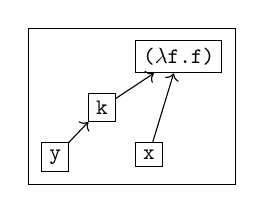
\begin{tikzpicture}[ scale=0.8, every node/.style={scale=0.8}, node distance = 0.25cm and 0.25cm]
      \node[draw=black] (e) {\texttt{($\lambda$f.f)}};

          \node[draw=black, below left = of e] (k) {\texttt{k}};
          \path[->] (k) edge node[left] {} (e);
            
              %\node[draw=black, below left = of k] (gamma1) {$\gamma_1$};
              %\path[->] (gamma1) edge node[left] {} (k);

              \node[draw=black, below left = of k] (y) {\texttt{y}};
              \path[->] (y) edge node[left] {} (k);

            %\node[draw=black, below right = of k] (gamma2) {$\gamma_2$};
            %\path[->] (gamma2) edge node[left] {} (k);

              \node[draw=black, below right = of k] (x) {\texttt{x}};
              \path[->] (x) edge node[left] {} (e);

          \node[draw,fill=none,scale=1.3,rectangle,fit=(e)(x)(y)](fbb){};
  \end{tikzpicture}
  \caption{Expression dependencies after evaluating \texttt{x}}
  \label{fig:dependencygraphv2}
\end{figure}
One consideration remains, the App rule does not promote lazy evaluation.
All non-trivial parameters must be bound to a variable by the Let rule to also allow anonymous expressions to be subject to lazy evaluation.
An algorithm for binding anonymous expressions can be found in~\cite{launchbury1993natural}.

\subsubsection{Dealing with ambiguity}
The rules so far have avoided dealing with variable ambiguity.
Notice that ambiguity can only arise in the Let rule, since the Let rule is the only rule of which can introduce new bindings to the heap.
Dealing with ambiguity is a matter of ensuring that variables are distinct.
Applying the technique from \autoref{sec:alpha} properly lets us evaluate programs without ambiguity.

Consider a previous case of variable capture \autoref{eq:ambg:cap}.
\begin{align}
  \texttt{\{x $\mapsto$ z, y $\mapsto$ x, $\dots$\}($\lambda$x.y) g}\label{eq:ambg:cap}
\end{align}
None of the changes so far have any impact on the falsity of the expression.
Consider that \texttt{x} and \texttt{y} must have entered the heap through a Let expression.
Consider also that some variable \texttt{k} cannot be subject to variable capture if \texttt{k $\notin$ Bound($\lambda$x.e)}.
Naturally if \texttt{k} is unique, that is, it is introduced through the \texttt{fresh} function from \autoref{sec:alpha} then \texttt{k} can never occur bound.
The obvious rule from these considerations must be new Let rule defined in \autoref{fig:eval:letrename}.
\begin{figure}[ht]
  \begin{mdframed}
    \begin{prooftree}
      \AxiomC{\texttt{$\Gamma$ $\cup$ \{$\gamma$ $\mapsto$ e\}, \{x $\mapsto$ $\gamma$\}p $\rightarrow$ $\Theta$, l}}
      \AxiomC{\texttt{$\gamma$ = fresh}}
        \RightLabel{Let}
        \BinaryInfC{\texttt{$\Gamma$, let x = e in p $\rightarrow$ $\Theta$, l}}
    \end{prooftree}   
  \end{mdframed}
  \caption{}
  \label{fig:eval:letrename}
\end{figure}
The correctness of \autoref{fig:eval:letrename} and the aforementioned considerations are formalised in~\cite{sestoft1997deriving}.

%For instance, consider the program in \autoref{lst:progambg} and the state after line \autoref{lst:progambg:l1} is executed in \autoref{eq:progambg2} and the remaining program in \autoref{lst:progambg2}.
%The state and remaining program is intact, but evaluating line \autoref{lst:progambg2:l1} in \autoref{lst:progambg} yields the state in \autoref{eq:progambg3} which changes the meaning of \texttt{v}.
%\begin{lstlisting}[language=ML,caption={Program which may suffer from variable ambiguity},label={lst:progambg},mathescape=true]
%let v = $\$$ (let x = 5 in ($\lambda$y.y + x)) in $\label{lst:progambg:l1}$
%let x = 0 in
%v 5
%\end{lstlisting}
%\begin{gather}
  %\texttt{\{v $\mapsto$ ($\lambda$y.y + x), x $\mapsto$ 5\}}\label{eq:progambg2}
%\end{gather}
%\begin{lstlisting}[language=ML,caption={Program after evaluating \texttt{v}},label={lst:progambg2},mathescape=true]
%let x = 0 in $\label{lst:progambg2:l1}$
%v 5
%\end{lstlisting}
%\begin{gather}
  %\texttt{\{v $\mapsto$ ($\lambda$y.y + x), x $\mapsto$ 0\}}\label{eq:progambg3}
%\end{gather}

%Naturally renaming can occur at the Let rule, since Let introduces new variables to the heap.
%Enhancing the Let rule with renaming by the semantics from \autoref{sec:alpha} yields a replacement for Let (\autoref{fig:eval:letrename})~\cite{sestoft1997deriving}. 
%Evaluating line \autoref{lst:progambg:l1} in \autoref{lst:progambg} now yields the state in \autoref{eq:pragambgfix} which introduces \texttt{x} as a fresh variable ($\gamma$) from the \texttt{fresh} function.
%\begin{gather}
  %\texttt{\{$\sigma$ $\mapsto$ ($\lambda$y.y + $\gamma$), $\gamma$ $\mapsto$ 5\}}\label{eq:pragambgfix}
%\end{gather}

\subsubsection{Introducing useful functionality}
As the set of rules stand currently one can express numbers through church encodings.
Church encodings provide a minimal and non-invasive set of combinators which allow the encoding of numbers.
Unfortunately it is not as practical as it is minimal to church encode numbers.
For instance, to represent the number \texttt{100000} one would require \texttt{100000} invocations of some successor function.
Fortunately dwelling on the representation of numbers is an easy task once one convinces themselves that ordinary numbers and arithmetic operations are friendly.

When discovering an arithmetic operations between two expressions, they must both be forced and then the pending expression must evaluated.
Clearly this rule is not encoded into the aforementioned rules, but can be modelled easily as shown in \autoref{fig:oplusrule}.
\begin{figure}[ht]
  \begin{mdframed}[style=style1]
        \begin{subfigure}[b]{1\textwidth}
        \vspace*{0.49cm}
          \begin{prooftree}
              \AxiomC{\texttt{$\Theta$, x $\rightarrow$ $\Sigma$, n}}
              \AxiomC{\texttt{$\Sigma$, y $\rightarrow$ S, t} $\,\,\,\,\,$ \texttt{$\oplus \in \{+,-,*,\backslash, =\}$}}
                \RightLabel{Bin op}
                \BinaryInfC{\texttt{$\Theta$, x $\oplus$ y $\rightarrow$ S, (n $\oplus$ t)}}
          \end{prooftree}   
        \end{subfigure}
        \begin{subfigure}[b]{1\textwidth}
        \vspace*{0.49cm}
            \begin{prooftree}
                \AxiomC{\texttt{n $\in \mathbb{Z^+}$}}
                \RightLabel{Num}
                \UnaryInfC{\texttt{S, n $\rightarrow$ S, n}}
            \end{prooftree}   
        \end{subfigure}
  \end{mdframed}
  \caption{}
  \label{fig:oplusrule}
\end{figure}
Notice that \autoref{fig:oplusrule} also must accompany a Num rule which introduces integers to the system.
\begin{remark}
  Notice that the Bin op rule in \autoref{fig:oplusrule} uses \texttt{x} and \texttt{y} which are in the domain of variables, since all non-trivial expressions must be bound to fresh names through Let.
\end{remark}

\begin{exmp}
Now that rules have been established which avoid variable ambiguity through renaming and support lazy evaluation, an example seems natural.
An expression which requires the aforementioned properties to resolve as expected is presented in \autoref{eq:doneexmp} and proved in \autoref{fig:finproofexmp}.
\begin{align}
  \texttt{let y = (1 + 1) in ($\lambda$x.($\lambda$y.x + y) x) y}\label{eq:doneexmp}
\end{align}
\begin{figure}[ht]
  \begin{mdframed}[style=bigbox]
    \begin{subfigure}[b]{1\textwidth}
      \vspace*{0.49cm}
      \begin{prooftree}
            \AxiomC{}
            \LeftLabel{Lam}
            \UnaryInfC{\texttt{\{$\gamma$ $\mapsto$ (1 + 1)\}, ($\lambda$x.($\lambda$y.x + y) x) $\rightarrow$ \{$\gamma$ $\mapsto$ (1 + 1)\},($\lambda$x.($\lambda$y.x + y) x)}}
      \end{prooftree}
      \caption{}
      \label{fig:finproofexmp:app1}
    \end{subfigure}
    \begin{subfigure}[b]{1\textwidth}
      \vspace*{0.49cm}
      \begin{prooftree}
            \AxiomC{}
            \LeftLabel{Lam}
            \UnaryInfC{\texttt{\{$\gamma$ $\mapsto$ (1 + 1)\}, ($\lambda$y.$\gamma$ + y) $\rightarrow$ \{$\gamma$ $\mapsto$ (1 + 1)\}, ($\lambda$y.$\gamma$ + y)}}
      \end{prooftree}
      \caption{}
      \label{fig:finproofexmp:app2}
    \end{subfigure}
    \begin{subfigure}[b]{1\textwidth}
      \vspace*{0.49cm}
      \begin{prooftree}
                \AxiomC{}
                \LeftLabel{Num}
                \UnaryInfC{\texttt{\{\}, 1 $\rightarrow$ \{\}, 1}}
                \AxiomC{}
                \LeftLabel{Num}
                \UnaryInfC{\texttt{\{\}, 1 $\rightarrow$ \{\}, 1}}
                \LeftLabel{Bin op}
                \BinaryInfC{\texttt{\{\}, 1 + 1 $\rightarrow$ \{\}, 2}}
                \LeftLabel{Var}
                \UnaryInfC{\texttt{\{$\gamma$ $\mapsto$ (1 + 1)\}, $\gamma$ $\rightarrow$ \{$\gamma$ $\mapsto$ 2\}, 2}}

                \AxiomC{}
                \RightLabel{Num}
                \UnaryInfC{\texttt{\{\}, 2 $\rightarrow$ \{\}, 2}}
                \RightLabel{Var}
                \UnaryInfC{\texttt{\{$\gamma$ $\mapsto$ 2\}, $\gamma$ $\rightarrow$ \{$\gamma$ $\mapsto$ 2\}, 2}}

              \LeftLabel{Bin op}
              \BinaryInfC{\texttt{\{$\gamma$ $\mapsto$ (1 + 1)\}, $\gamma$ + $\gamma$ $\rightarrow$ \{$\gamma$ $\mapsto$ 2\}, 4}}
      \end{prooftree}
      \caption{}
      \label{fig:finproofexmp:bin}
    \end{subfigure}
    \begin{subfigure}[b]{1\textwidth}
      \vspace*{0.49cm}
      \begin{prooftree}
            \AxiomC{\autoref{fig:finproofexmp:app1}}
              \AxiomC{\autoref{fig:finproofexmp:app2}}
              \AxiomC{\autoref{fig:finproofexmp:bin}}
              \LeftLabel{App}
            \BinaryInfC{\texttt{\{$\gamma$ $\mapsto$ (1 + 1)\}, ($\lambda$y.$\gamma$ + y) $\gamma$ $\rightarrow$ \{$\gamma$ $\mapsto$ 2\}, 4}}
          \LeftLabel{App}
          \BinaryInfC{\texttt{\{$\gamma$ $\mapsto$ (1 + 1)\}, ($\lambda$x.($\lambda$y.x + y) x) $\gamma$ $\rightarrow$ \{$\gamma$ $\mapsto$ 2\}, 4}}
        \LeftLabel{Let}
        \UnaryInfC{\texttt{\{\}, let y = (1 + 1) in ($\lambda$x.($\lambda$y.x + y) x) y $\rightarrow$ \{$\gamma$ $\mapsto$ 2\}, 4}}
      \end{prooftree}
      \caption{}
      \label{fig:finproofexmp:all}
    \end{subfigure}
  \end{mdframed}
  \caption{The proof for the program in \autoref{eq:doneexmp}}
  \label{fig:finproofexmp}
\end{figure}
Notice that the left branch and right branch in \autoref{fig:finproofexmp:bin} are not identical.
The left branch saves the evaluation result such that the right branch only requires a lookup to find $\gamma$.
\end{exmp}


%The $\cup$ operator merges two substitution mappings, choosing the leftmost mapping on duplicates, such that \texttt{\{x $\mapsto$ y, z $\mapsto$ h\} $\cup$ \{x $\mapsto$ m\} $\rightarrow$ \{x $\mapsto$ y, z $\mapsto$ h\}}, such that the semantics of $\cup$ satisfy \autoref{eq:subsemfixed}.
%More generally, a simple rule for App could be defined as in \autoref{fig:simpleapp} which states ``Evaluate \texttt{($\lambda$x.e) z} with the substitution mapping \texttt{S} to \texttt{y} with the substitution mapping $\Sigma$ by first evaluating \texttt{e} with the substitution mapping \texttt{S} $\cup$ \texttt{\{x $\mapsto$ z\}} to \texttt{y} with the substitution mapping $\Sigma$''.
%\begin{figure}[ht]
%\begin{lstlisting}[language=ML,caption={Problematic program},label={lst:problemprog},mathescape=true]
%fun f a = 
  %fun g x = 
    %let a = 20;
    %a + x;
  %(g a) + a;
%f 10;
%\end{lstlisting}
%\end{figure}
%Evaluating \autoref{lst:problemprog}, using the rules proposed in \autoref{fig:rules:env}, yields an interesting case of variable ambiguity.
%At some point the evaluation machine will reach a state with the expression \texttt{(g a) + a} and substitution mapping \texttt{\{a $\mapsto$ 10, g $\mapsto$ ($\lambda$x.let a = 20 in (a + x))\}}.
%By the laws of commutativity for addition, it should be possible pick either of the two expressions to evaluate first.
%If any one of the branches in the addition operator are side-effectful, it may become a problem, but this language only deals with pure programs.
%Evaluating the left side of \texttt{(g a) + a} first, yields \texttt{30 + a} with the substitution mapping \texttt{\{a $\mapsto$ 20, g $\mapsto$ $\dots$\}}, and finally \texttt{50}.
%Evaluating the right side of \texttt{(g a) + a} first, yields \texttt{(g a) + 10} with the substitution mapping \texttt{\{a $\mapsto$ 10, g $\mapsto$ $\dots$\}}, and finally \texttt{40}.
%Clearly the order of evaluation is of importance for the result, which is often not the desired semantics.
%If there exists multiple reduction techniques which ensure the same result, the system is called \textit{confluent}.
%The reduction rules for the lambda calculus programs are confluent~\cite{church1936some}, which implies that the current set of rules are not valid evaluation rules for the lambda calculus.
%%If reduction strategies for the lambda calculus are not confluent, programs become difficult to reason with.
%If the rules were to be confluent, any reduction order would result in \texttt{40}.
%The different results are an effect of leaking the substitution mapping to the outside of the lexical scope in which it was used.
%A simple solution could involve saving the substitution mapping once the machine enters an abstraction, then restore the same substitution mapping when it leaves.
%\begin{figure}[ht]
    %\begin{mdframed}[style=style1]
        %\vspace*{0.4cm}
          %\begin{prooftree}
            %\AxiomC{\texttt{$\Theta$, f $\rightarrow$ S, ($\lambda$x.e)}}
            %\AxiomC{\texttt{S $\cup$ \{x $\mapsto$ z\}, e $\rightarrow$ $\Sigma$, y}}
              %\RightLabel{App}
              %\BinaryInfC{\texttt{$\Theta$, f z $\rightarrow$ $\Theta$, y}}
          %\end{prooftree}   
    %\end{mdframed}
    %\caption{An application rule which does not leak}
    %\label{fig:cleanapp}
%\end{figure}
%\noindent \autoref{fig:cleanapp} is a slightly modified version of \autoref{fig:rules:env:app}, with the difference of requiring the resulting substitution mapping to be the initial substitution mapping.

%\autoref{fig:cleanapp} does not handle closure correctly.
%Evaluating \autoref{lst:closprob} under the rules defined in \autoref{fig:cleanapp} yields yet another problem.
%\begin{figure}[ht]
%\begin{lstlisting}[language=ML,caption={Program with closure},label={lst:closprob},mathescape=true]
%fun g x =
  %fun f z = x + z; // closes x
  %fun run y =
    %let x = 20; $\label{closov}$
    %f y;
  %run 10;
%g 3;
%\end{lstlisting}
%\end{figure}
%When line \autoref{closov} is reached in \autoref{lst:closprob}, then \texttt{x} in the substitution mapping is overwritten by the rules in \autoref{fig:cleanapp}.
%Even if renaming is performed such that all variables become unique, recursive functions still remain a problem.
%Taking a step back and considering what the evaluation strategy which involves eager substitution implies.
%The \textit{first} substitution mapping which reaches an expression, is the substitution mapping which is relevant for that expression.
%By these semantics substitution mappings must be paired with expressions and should now be read as ``\texttt{S, e} are the pair of the environment \texttt{S} necessary to evaluate the expression \textit{e}''.
%Substitutions bound to expressions should remain immutable; whenever an expression is discovered during interpretation, the substitution at that time is the only important substitution mapping.
%The $\cup$ operator for two substitutions should now be inverted, that is, \texttt{S $\cup$ $\Sigma$} should now pick substitutions from \texttt{S} if duplicates occur.
%Furthermore, notice that binding substitutions to expressions also allows substitutions to float up throughout interpretation.
%Now the application rule must implement \autoref{eq:subsemfixed}, seen in \autoref{fig:subsapp}.
%\begin{figure}[ht]
    %\begin{mdframed}[style=bigbox]
        %\vspace*{0.4cm}
          %\begin{prooftree}
            %\AxiomC{\texttt{$\Theta$, f $\rightarrow$ S, ($\lambda$x.e)}}
            %\AxiomC{\texttt{\{x $\mapsto$ (S, z)\} $\cup$ S, e $\rightarrow$ ($\Sigma$ $\backslash$ \{x\}) $\cup$ S, y}}
              %\RightLabel{App}
              %\BinaryInfC{\texttt{$\Theta$, f z $\rightarrow$ $\Sigma$, y}}
          %\end{prooftree}   
    %\end{mdframed}
    %\caption{An application rule which implements \autoref{eq:subsemfixed} and paired substitutions.
    %% (the entire set of rules can be found in \autoref{fig:subrenam})
    %}
    %\label{fig:subsapp}
%\end{figure}
%\begin{remark}
  %An interesting observation is that these semantics introduce expressions with closures as a construct similar to classes in object oriented languages.
  %\texttt{e} is an abstract representation of something, while the environment \texttt{S} is the necessary values to instantiate \texttt{e}, together they can produce some output.
  %Curried functions can also be seen this way, yet it remains an interesting observation.
%\end{remark}

%\noindent Consider the previously discussed program and state in \autoref{eq:tabc}.
%\begin{align}
  %\texttt{\{x $\mapsto$ (S, z), y $\mapsto$ ($\Theta$, x), $\dots$\}($\lambda$x.y) g} \label{eq:tabc}
%\end{align}
%Performing the next two iterations such that the next states become \autoref{eq:tabd} and then finally \autoref{eq:tabe}.
%\begin{gather}
  %\texttt{\{x $\mapsto$ ($\Sigma$, g), y $\mapsto$ ($\Theta$, x), $\dots$\}y} \label{eq:tabd}\\
  %\texttt{$\Theta$ x} \label{eq:tabe}
%\end{gather}
%The program now evaluates as intended which is a consequence of binding all expressions with their environments.

%Surely \autoref{fig:subsapp} solves the problem of lazy substitutions, but alas this is not yet the case.
%To reach a set of rules which will guarantee lazy substitutions and allow call by need, an additional ingredient is needed.
%To understand the need for this ingredient, consider the following valid state \texttt{\{x $\mapsto$ z, y $\mapsto$ x\} ($\lambda$x.y) g} in the context of \autoref{fig:subsapp}.
%When visiting \texttt{($\lambda$x.y)} then the following substitution mapping is applied \texttt{\{x $\mapsto$ g\}}.
%Once \texttt{y} is visited the substitution mapping will be \texttt{\{x $\mapsto$ g, y $\mapsto$ x\}}, substituting again yields \texttt{x} which becomes \texttt{g} which does not necessarily satisfy \texttt{g $\equiv$ z}.
%One could rename all variables in some phase in compilation, but the case for recursion is not handled since a duplicate variable name can occur.
%Consider the program in \autoref{lst:amgprog} which yields an invalid state during interpretation.
%\begin{figure}[ht]
%\begin{lstlisting}[language=ML,caption={Recursive program with ambiguity},label={lst:amgprog},mathescape=true]
%fun f x = 
  %f (x + x); $\label{lst:amgprog:l2}$
%f 10;
%\end{lstlisting}
%\end{figure}
%Once Line \autoref{lst:amgprog:l2} is reached the first time, the program will have the state \texttt{\{$\dots$, x $\mapsto$ 10\}}.
%On the second iteration, the program will have the state \texttt{\{$\dots$, x $\mapsto$ (x + x)\}}, which does not make sense.

%, thus the expression is equivalent to \texttt{($\lambda$x.x) g}, which is not necessarily correct in the case that \texttt{z $\neq$ g}.

%\autoref{fig:cleanapp} does not handle recursion that well, under normal order evaluations, which becomes apparent in expressions such as \texttt{let f = ($\lambda$f.$\lambda$x.if (x == 0) 0 (x + (f (x - 1))) in f f n)}.
%Once the base case is reached (\texttt{x == 0}), then some expression has accumulated in the substitution set \texttt{\{x $\mapsto$ x + ((x - 1) + $\dots$ + ((x - 1) - 1 $\dots$))\}}, which is clearly not valid.
%\begin{figure}[ht]
    %\begin{mdframed}[style=style1]
        %\vspace*{0.4cm}
          %\begin{prooftree}
            %\AxiomC{\texttt{S $\cup$ \{x $\mapsto$ Sz\}, e $\rightarrow$ $\Sigma$, y}}
              %\RightLabel{App}
              %\UnaryInfC{\texttt{S, ($\lambda$x.e) z $\rightarrow$ S, y}}
          %\end{prooftree}   
    %\end{mdframed}
    %\caption{An application rule which works for recursion}
    %\label{fig:recapp}
%\end{figure}
%\noindent The problem of recursion can be solved by never introducing variables, but instead always substituting them thus mapping to the value (\autoref{fig:recapp}).
%An unfortunate consideration which yields \autoref{fig:recapp} unsatisfactory, under the current semantics, is that \texttt{z} can also be bound to an expression which is not a variable, like an application for instance (parameters are never evaluated first in normal order).
%One could recursively apply substitutions to \texttt{z}, but then the \textit{suspense} would be broken.
%\begin{remark}
  %When considering an arbitrarily large expression under call by name (or need), there is no guarantee that the expression will ever be evaluated, that is, a suspended expression being evaluated.
  %Therefore substituting expressions eagerly might compromise performance guarantees.
  %Furthermore consider substituting an expression which contains conditional branches, one branch might be a single expression and the other might be a very large expression.
  %If the program never picks the large expression, it should never have any impact on performance.
%\end{remark}
%\noindent For this method to work then substitutions must be applied lazily.
%The notion of substitutions should now be changed such that substitutions are performed recursively and lazily (\autoref{eq:subsemlaz}).
%\begin{align}
  %&\{ x \mapsto y \} x = y \label{eq:subsemlaz}\\
  %&\{ x \mapsto y \} z = z  \tag*{}\\
  %&S f z = (Sf)(Sz) \tag*{}\\
  %&S (\lambda x.e) = (\lambda x.Se) \label{eq:subsemlaz2} %& (x \mapsto y) \notin S \tag*{}%\\
  %%&S (\lambda x.e) = (\lambda x.(S \backslash \{x \mapsto y\})e) & (x \mapsto y) \in S \tag*{}%\label{eq:subsemlaz2}
%\end{align}
%Note that previously the substitution mappings travelled along with the interpreter while interpreting, but now substitution mappings should travel along variables.
%Expressions should now be modelled by a pair \texttt{S,e}, where \texttt{S} is a substitution mapping which should be considered once \texttt{e} is evaluated. 
%If a substitution mapping \texttt{S} is applied and then a substitution mapping $\Sigma$ is applied, then the resulting set for an expression should become \texttt{S $\cup$ $\Sigma$}.
%The order in which substitution mappings are combined is of importance since the ``most recent'' substitution mapping should contain the lexically ``closest'' variables.
%\begin{remark}
  %The union of two substitution mappings is important since applying them sequentially could damage the asymptotic complexity of substitution.
  %Clearly the variables which are lexically ``closer'' must also be respected. % but this is not of significant importance since $\alpha$-conversion will become necessary later.
  %If $n$ substitutions \texttt{S$_1 \dots$ S$_n$} are applied efficiently ($O(1)$ lookup), then the total number of operations will be $n$, whereas if the substitutions were unioned as they were created the work would be constant.
  %An interpreter would not be of much value if a recursive function which recurses $n$ times takes $O(n^2)$ time, since $O(1 + 2  \dots + n) = O(n \frac{n + 1}{2}) = O(n^2)$.
%\end{remark}
%\begin{figure}[ht]
    %\begin{mdframed}[style=style1]
        %\vspace*{0.4cm}
          %\begin{prooftree}
            %\AxiomC{\texttt{\{x $\mapsto$ $\Sigma$,z\} e $\rightarrow$ $\Theta$,y}}
              %\RightLabel{App}
              %\UnaryInfC{\texttt{S,($\lambda$x.e) z $\rightarrow$ $\Theta$,y}}
          %\end{prooftree}   
    %\end{mdframed}
    %\caption{An application rule which has abstracted away substitution mappings}
    %\label{fig:recappsimple}
%\end{figure}
%%\autoref{eq:subsemlaz2} has been introduced for completeness, but can be omitted since it cannot occur in the lazy substitution model, since the only method which carries the substitution mapping into an abstraction is an application.
%Notice that any variables introduced must be so through applications.
%All the substitution work can now be moved into the introduced variable (\autoref{fig:recappsimple}).

%Functions can store intermediate values in two ways, either by partial application or closure.
%When partially applying functions, the intermediate values (and their respective variable bindings) must be saved in a safe and isolated way.
%Surely a system which uses \autoref{fig:recappsimple} is confluent, but, alas this is not the case.
%\texttt{let f = ($\lambda$x.$\lambda$y.x + y) 0 in E} shows a partially applied function \texttt{f} which should have \texttt{x} binded to the expression \texttt{0} in such a way that applying another value to \texttt{f} will finalize the value.
%Letting \texttt{E} satisfy \texttt{x $\notin$ Free(E)} while \texttt{x} occurs in \texttt{E}, that is, \texttt{x} is bound in \texttt{E}, provides an interesting problem for interpreters under call by value.
%If we let \texttt{f} be eager, that is, the binding of \texttt{x} to the expression \texttt{0} is not suspended, then \texttt{f} must associate itself with the substitution \texttt{\{x $\mapsto$ 0\}} and \textit{never} let any other substitutions override the variable \texttt{x}.
%\begin{remark}
  %Ad-hoc eager evaluation, that is, forcing suspended evaluations by use of some symbol is often allowed in functional programming languages.
  %Explicit forcing of suspended computations is a technique often used when creating data structures with good worst case performance.
%\end{remark}
%\noindent Now let \texttt{E} be \texttt{($\lambda$x.let g = f in g) 10} such that an evaluation yields \autoref{eq:red}.
%\begin{align}
  %&\texttt{S = \{x $\mapsto$ 10, f $\mapsto$ \{x $\mapsto$ 0\}($\lambda$y.x + y)\}} \tag*{}\\
  %&\texttt{S(let g = f in g)} \label{eq:red}\\
  %&\texttt{S($\lambda$g.g) S(f)} \tag*{}\\
  %&\texttt{($\lambda$g.S(g)) \{x $\mapsto$ 0\}($\lambda$y.x + y)} \tag*{}\\
  %&\texttt{(\{x $\mapsto$ 0\} $\cup$ S)($\lambda$y.x + y)} \tag*{}\\
  %&\texttt{S($\lambda$y.x + y)} \tag*{}\\
  %&\texttt{\{$\dots$, x $\mapsto$ 10\}($\lambda$y.x + y)} \tag*{}
%\end{align}
%\autoref{eq:red} is a textbook closure and partial application problem in disguise.
%Consider the following valid state \texttt{\{x $\mapsto$ z, y $\mapsto$ x\} ($\lambda$x.y) g} in the context of \autoref{fig:cleanapp}.
%When visiting \texttt{($\lambda$x.y)} then the following substitution mapping is applied \texttt{\{x $\mapsto$ g\}}.
%Once \texttt{y} is visited the substitution mapping will be \texttt{\{x $\mapsto$ g, y $\mapsto$ x\}}, thus the expression is equivalent to \texttt{($\lambda$x.x) g}, which is not necessarily correct in the case that \texttt{z $\neq$ g}.
%Both problems are an effect of variable ambiguity.

%We almost have all the building blocks in place now.
%Temporarily assuming that substitutions occur eagerly yields interesting results which will help finalize the model.
%Let \texttt{((($\lambda$x.$\lambda$y.$\lambda$x.x) 1) 2) 3} be an expression which is to be evaluated.
%If we follow the rules in \autoref{eq:subsemlaz} then the first substitution will yield.
%\[
  %\texttt{\{x $\mapsto$ 3\}(($\lambda$y.$\lambda$x.x) 1) 2} \rightarrow \texttt{(($\lambda$y.$\lambda$x.3) 1) 2}
%\]
%Adding a rule which allows only the innermost substitution to be captured yields the two following rules (\autoref{eq:subsemfixed2}) instead of \autoref{eq:subsemlaz2}.
%\begin{align}
  %&S (\lambda x.e) = (\lambda x.Se) \label{eq:subsemfixed2} & (x \mapsto y) \notin S \tag*{}\\
  %&S (\lambda x.e) = (\lambda x.(S \backslash \{x \mapsto y\})e) & (x \mapsto y) \in S \tag*{}%\label{eq:subsemlaz2}
%\end{align}


%\autoref{fig:recappsimple} solves the problem of not letting substituted to values have their meaning changed, by pairing expressions with their entire substitution mapping.

%\autoref{fig:recappsimple} induces rather complicated programs to reason with since substitution mapping can occur within substitution mappings.
%Attempting to extend \autoref{fig:recappsimple} further, to solve variable ambiguity, sacrifices algorithmic elegance and simplicity further.
%Taking a step back and considering what closures and partial application need to behave deterministically is rooted in solving variable ambiguity.
%Instead, if all variables are unique, ambiguity cannot occur.
%By renaming all variables to a unique name when they are introduced, the evaluation model can be simplified significantly and allows \textit{any} of the aforementioned application rules (some of which imply eager substitution).
%The operation of renaming is called an $\alpha$-conversion.
%The shortcomings of \autoref{fig:simpleapp} become more apparent once one begins to consider more exotic evaluation strategies, namely call by need.
%Looking at call by need from a philosophical perspective, indicates that reduction rules must support returning information about newly computed variable values ``up'' through the evaluation tree.
%Furthermore when returning these modified variables up through the program tree, all variables which point to the same expression must also be updated.
%\\
%The next step in correctly evaluating the lambda calculus is applying \textit{$\alpha$-conversions} which is the operation of renaming.
%\subsubsection{$\alpha$-conversions}
%The $\alpha$-conversion mapping can occur as the substitution mapping, that is \texttt{\{x $\mapsto$ $\gamma_1$, y $\mapsto$ $\gamma_2$\}}; $\alpha$-conversions are philosophical constructs more than materialized mappings.
%$\alpha$-conversions guarantee what is called \textit{$\alpha$-equivalence} which is the notion of semantic equivalence.
%For instance \texttt{$\lambda$x.x} is $\alpha$-equivalent with \texttt{$\lambda\gamma.\gamma$} since both expressions are semantically equivalent.
%%$\alpha$-conversions solve some critical problems such as closures and recursion when evaluating the lambda calculus.
%%$\alpha$-conversions should also be non-destructive but still be context aware such that when leaving an abstraction the remaining substitution mapping is a superset of the substitution mapping when entering.
%%More formally if \texttt{S, e $\rightarrow$ $\Sigma$, e'} then $\{x \,\,|\,\, (x \mapsto y) \in S\} \subseteq \{x \,\,|\,\, (x \mapsto y) \in \Sigma\}$.
%\begin{lstlisting}[language=ML,caption={Recursive addition function},label={lst:recalpha},mathescape=true]
%let f = ($\lambda$f'.$\lambda$x.
    %if (x = 0) x else f' f' ((x - 1) + (x - 1))) in
%f f 10
%\end{lstlisting}
%%A strong guarantee that can be made by tuning the evaluation strategy which is particularly useful for $\alpha$-conversion algorithms is that \textit{any} returned value has had \textit{every} term that it contains visited.
%%An algorithm for performing $\alpha$-conversions can be implemented that picks a new variable name from any infinite domain when an abstraction has had a value applied to it and replaces future encountered variables with the new one, such an algorithm only works if the guarantee of visiting every term is made.
%%The algorithm should also introduce the applied value to the substitution set through the alpha converted name.
%\noindent An $\alpha$-conversion algorithm can be implemented such that when a new variable is introduced through an abstraction, a new name for the variable is given.
%More formally; Let $V_1$ be the domain of variables in the program and $V_2$ be the infinite domain for variable names that satisfies $V_1 \cap V_2 = \emptyset$, then when a new variable \texttt{x} is discovered, replace it with some $\gamma \in V_2$ and let $V_2 = V_2 \backslash \{\gamma\}$. 
%For instance, let \texttt{($\lambda\gamma_1$.$\lambda\gamma_2$.if ($\gamma_2$ = 0) $\gamma_2$ else $\gamma_1$ $\gamma_1$ (($\gamma_2$ - 1) + ($\gamma_2$ - 1)))} be the $\alpha$-converted version of \texttt{f} in \autoref{lst:recalpha}.
%It should become clear that an $\alpha$-conversion algorithm must also follow the reduction order or else one can force terrible runtime in a call by name (or need) environment by creating purposeless terms which are never executed but are converted.
%$\alpha$-conversions must be suspended until it is needed; let $\alpha E$ denote the $\alpha$-conversion for some conversion mapping $\alpha$ on a lambda expression $E$ which lazily $\alpha$-converts $E$.
%The replacement rules for $\alpha$-conversions are the same as for substitutions.
%\begin{align}
  %&\texttt{[x $\mapsto$ y]x = y} &\label{eq:alpharep}\\
  %&\texttt{[x $\mapsto$ y]z = z} &\tag*{}\\
  %&\texttt{$\alpha$(f z) = ($\alpha$f)($\alpha$z)} &\tag*{}\\
  %&\texttt{$\alpha$($\lambda$x.e) = ($\lambda$x.$\alpha$e)} & \texttt{(x $\mapsto$ y) $\notin$ $\alpha$} \tag*{}\\
  %&\texttt{$\alpha$($\lambda$x.e) = ($\lambda$x.($\alpha\backslash$[x $\mapsto$ y])e)} & \texttt{(x $\mapsto$ y) $\in$ $\alpha$} \label{eq:alprepsub}
%\end{align}

%We almost have all the building blocks in place now.
%The problem of ambiguity between \textit{different} variables, that is, variables different places in the program with the same name and in recursion, can now be solved.
%Once again, not breaking suspension remains as an interesting value.
%In \autoref{fig:subrenam} the \texttt{fresh} function picks a new variable from $V_2$ and updates $V_2$ such that picked variable no longer exists in $V_2$.
%\begin{figure}[ht]
    %\begin{mdframed}[style=bigbox]
        %\vspace*{0.49cm}
        %\begin{subfigure}[b]{0.38\textwidth}
            %\begin{prooftree}
                %\AxiomC{}
                %\RightLabel{Abs}
                %\UnaryInfC{\texttt{S, ($\lambda$x.e) $\rightarrow$ S, ($\lambda$x.e)}}
            %\end{prooftree}   
            %\caption{}
          %\label{fig:rules:freshenv:abs}
        %\end{subfigure}
        %\begin{subfigure}[b]{0.58\textwidth}
            %\begin{prooftree}
              %\AxiomC{\texttt{Sx $\equiv$ x}}
                %\RightLabel{Var (terminal)}
                %\UnaryInfC{\texttt{S, x $\rightarrow$ S, x}}
            %\end{prooftree}   
            %\caption{}
          %\label{fig:rules:freshenv:varterm}
        %\end{subfigure}
        %\begin{subfigure}[b]{1\textwidth}
        %\vspace*{0.49cm}
            %\begin{prooftree}
              %\AxiomC{\texttt{$\Theta$, y $\rightarrow$ $\Sigma$, e}}
                %\RightLabel{Var}
                %\UnaryInfC{\texttt{\{x $\mapsto$ ($\Theta$, y)\} $\cup$ S, x $\rightarrow$ \{x $\mapsto$ ($\Theta$, e)\} $\cup$ $\Sigma$, e}}
            %\end{prooftree}   
            %\caption{}
          %\label{fig:rules:freshenv:var}
        %\end{subfigure}
        %\begin{subfigure}[b]{1\textwidth}
          %\vspace*{0.4cm}
              %\vspace*{0.4cm}
              %\begin{prooftree}
                %\AxiomC{\texttt{$\Theta$, f $\rightarrow$ S, ($\lambda$x.e)}}
                %\AxiomC{\texttt{\{x $\mapsto$ (S, z)\} $\cup$ S, e $\rightarrow$ ($\Sigma$ $\backslash$ \{x\}) $\cup$ S, y}}
                  %\RightLabel{App}
                  %\BinaryInfC{\texttt{$\Theta$, f z $\rightarrow$ $\Sigma$, y}}
              %\end{prooftree}   
          %\caption{An application rule which binds the current environment to expressions}
          %\label{fig:rules:freshenv:app}
        %\end{subfigure}
    %\end{mdframed}
    %\caption{A set of rules which support the desired semantics}
    %\label{fig:subrenam}
%\end{figure}
%\begin{figure}[ht]
%\end{figure}

%First consider the implications of an eager $\alpha$-conversion strategy in \autoref{eq:alpharep}.
%Applying $\alpha$-conversions in applications eagerly ensures that all references to the applied to variable is are replaced (\autoref{fig:simpleappalpha}).
%Also notice that \autoref{eq:alprepsub} ensures that only variables that reference the replaced variable are renamed.
%\begin{figure}[ht]
    %\begin{mdframed}[style=style1]
        %\vspace*{0.4cm}
          %\begin{prooftree}
            %\AxiomC{\texttt{$\gamma$ = fresh \,\,\,\,\, S $\cup$ \{$\gamma$ $\mapsto$ z\}, [x $\mapsto$ $\gamma$]e $\rightarrow$ $\Sigma$, y}}
              %\RightLabel{App}
              %\UnaryInfC{\texttt{S, ($\lambda$x.e) z $\rightarrow$ $\Sigma$, y}}
          %\end{prooftree}   
    %\end{mdframed}
    %\caption{The simple application rule with $\alpha$-conversions}
    %\label{fig:simpleappalpha}
%\end{figure}
%The semantics of eager $\alpha$-conversion implies that once an $\alpha$-conversion is converting an expression, all free variables which the $\alpha$-conversion addresses should be renamed eagerly.
%Moreover, this implies that if some $\alpha$-conversion $\alpha_1$ suspends conversion of an expression and then some other conversion $\alpha_2$ suspends a conversion on the same expression, $\alpha_1$'s conversions should take precedence.
%That is, suspended conversions cannot have their conversions overwritten by other conversions such that \texttt{[x $\mapsto$ y] $\cup$ [x $\mapsto$ z, $\gamma$ $\mapsto$ k] = [x $\mapsto$ y, $\gamma$ $\mapsto$ k]}.

%\begin{lstlisting}[language=ML,caption={$\alpha$-conversion of a program with variable name collisions},label={lst:ambg},mathescape=true]
%($\lambda$x.$\lambda$y.$\lambda$x.x + y) $\rightarrow$ ($\lambda\gamma$.$\lambda\theta$.$\lambda\sigma$.$\sigma$ + $\theta$)
%\end{lstlisting}

%In \autoref{subfig:red4} the application which contains \texttt{$\lambda$f'} and \texttt{f'} as children (the red node) must $\alpha$-convert \texttt{f'} in ``this scope''.
%If \texttt{f'} is not $\alpha$-converted a circular dependency will arise $S = \{ \gamma \mapsto \texttt{f'} \}, \alpha = [ \texttt{f'} \mapsto \gamma ]$.

%\begin{exmp}
  %\autoref{fig:red:exmp} is an example of an iteration of \autoref{lst:recalpha}.
%\begin{figure}
    %\centering
    %\begin{subfigure}[b]{0.49\textwidth}
        %\centering
        %\begin{tikzpicture}[ scale=0.8, every node/.style={scale=0.8}, node distance = 0.15cm and 0.15cm]
                %\node[draw=black] (app1) {\texttt{app}};
                    %\node[draw=black, below right = of app1] (var1) {\texttt{10}};
                    %\path[-] (app1) edge node[left] {} (var1);

                    %\node[draw=black, below left = of app1] (app2) {\texttt{app}};
                    %\path[-] (app1) edge node[left] {} (app2);
                        %\node[draw=red, below left = of app2] (f1) {\texttt{f}};
                        %\path[-] (app2) edge node[left] {} (f1);
                        %\node[draw=black, below right = of app2] (f2) {\texttt{f}};
                        %\path[-] (app2) edge node[left] {} (f2);

                %\node[draw,scale=1.3,fill=none,rectangle,fit=(app1)(f1)(var1)](fstB){};
                %\path (fstB.north east) -- (fstB.south east) coordinate[midway] (fstP);
        %\end{tikzpicture}
        %\caption{
          %\texttt{S = \{f $\mapsto$ ($\lambda$f'.$\lambda$x.if (x = 0) x else f' f' (x - 1))\}}
        %}
    %\end{subfigure}
    %\begin{subfigure}[b]{0.49\textwidth}
        %\centering
        %\begin{tikzpicture}[ scale=0.8, every node/.style={scale=0.8}, node distance = 0.15cm and 0.15cm]
                %\node[draw=black] (app1) {\texttt{app}};
                    %\node[draw=black, below right = of app1] (var1) {\texttt{10}};
                    %\path[-] (app1) edge node[left] {} (var1);

                    %\node[draw=black, below left = of app1] (app2) {\texttt{app}};
                    %\path[-] (app1) edge node[left] {} (app2);
                        %\node[draw=red, below left = of app2] (lam1) {\texttt{$\lambda$f'}};
                        %\path[-] (app2) edge node[left] {} (lam1);
                            %\node[draw=black, below = of lam1] (lam2) {\texttt{$\lambda$x}};
                            %\path[-] (lam1) edge node[left] {} (lam2);
                                %\node[draw=black, below = of lam2] (app3) {\texttt{app}};
                                %\path[-] (lam2) edge node[left] {} (app3);
                                    %\node[draw=black, below left = of app3] (app4) {\texttt{app}};
                                    %\path[-] (app3) edge node[left] {} (app4);
                                        %\node[draw=black, below left = of app4] (app5) {\texttt{app}};
                                        %\path[-] (app4) edge node[left] {} (app5);
                                            %\node[draw=black, below left = of app5] (if) {\texttt{if}};
                                            %\path[-] (app5) edge node[left] {} (if);
                                            %\node[draw=black, below right = of app5] (ifc) {\texttt{x = 0}};
                                            %\path[-] (app5) edge node[left] {} (ifc);
                                        %\node[draw=black, below right = of app4] (ift) {\texttt{x}};
                                        %\path[-] (app4) edge node[left] {} (ift);
                                    %\node[draw=blue, below right = 0.15cm and 0.6cm of app3] (iff) {\texttt{f' f' ((x - 1) + (x - 1))}};
                                    %\path[-] (app3) edge node[left] {} (iff);
                        %\node[draw=black, below right = of app2] (f2) {\texttt{f}};
                        %\path[-] (app2) edge node[left] {} (f2);

                %\node[draw,fill=none,scale=1.3,rectangle,fit=(app1)(if)(ifc)(var1)(iff)](sndB){};
                %%\path (sndB.north west) -- (sndB.south west) coordinate[midway] (sndP);
            %\end{tikzpicture}
            %\caption{
                %\texttt{$\Sigma$ = S}
            %}
    %\end{subfigure}
    %%\tikz[overlay,remember picture]{\draw [->] (fstP) -- (fstP-|sndP);}
    %\begin{subfigure}[b]{0.49\textwidth}
        %\centering
        %\begin{tikzpicture}[ scale=0.8, every node/.style={scale=0.8}, node distance = 0.15cm and 0.15cm]
                                %\node[draw=black, below = of lam2] (app3) {\texttt{app}};
                                    %\node[draw=black, below left = of app3] (app4) {\texttt{app}};
                                    %\path[-] (app3) edge node[left] {} (app4);
                                        %\node[draw=black, below left = of app4] (app5) {\texttt{app}};
                                        %\path[-] (app4) edge node[left] {} (app5);
                                            %\node[draw=black, below left = of app5] (if) {\texttt{if}};
                                            %\path[-] (app5) edge node[left] {} (if);
                                            %\node[draw=black, below right = of app5] (ifc) {\texttt{x = 0}};
                                            %\path[-] (app5) edge node[left] {} (ifc);
                                        %\node[draw=black, below right = of app4] (ift) {\texttt{x}};
                                        %\path[-] (app4) edge node[left] {} (ift);
                                    %\node[draw=blue, below right = 0.15cm and 0.6cm of app3] (iff) {\texttt{f' f' ($\dots$)}};
                                    %\path[-] (app3) edge node[left] {} (iff);
                %\node[draw,fill=none,scale=1.3,rectangle,fit=(app3)(if)(ifc)(iff)](fouB){};
                %%\path (sndB.north west) -- (sndB.south west) coordinate[midway] (sndP);
            %\end{tikzpicture}
            %\caption{
                %\\
                %\texttt{$\Theta_0$ = \{f' $\mapsto$ ($\Sigma$, f)\} $\cup$ $\Sigma$}\\
                %\texttt{$\Theta$ = \{x $\mapsto$ ($\Theta_0$, 10)\} $\cup$ $\Theta_0$}
            %}
    %\end{subfigure}
    %\begin{subfigure}[b]{0.49\textwidth}
        %\centering
        %\begin{tikzpicture}[ scale=0.8, every node/.style={scale=0.8}, node distance = 0.15cm and 0.15cm]
                %\node[draw=blue] (app1) {\texttt{app}};
                    %\node[draw=black, below right = of app1] (var1) {\texttt{x - 1}};
                    %\path[-] (app1) edge node[left] {} (var1);

                    %\node[draw=purple, below left = of app1] (app2) {\texttt{app}};
                    %\path[-] (app1) edge node[left] {} (app2);
                        %\node[draw=black, below left = of app2] (lam1) {\texttt{$\lambda$f'}};
                        %\path[-] (app2) edge node[left] {} (lam1);
                            %\node[draw=black, below = of lam1] (lam2) {\texttt{$\lambda$x}};
                            %\path[-] (lam1) edge node[left] {} (lam2);
                                %\node[draw=black, below = of lam2] (app3) {\texttt{app}};
                                %\path[-] (lam2) edge node[left] {} (app3);
                                    %\node[draw=black, below left = of app3] (app4) {\texttt{app}};
                                    %\path[-] (app3) edge node[left] {} (app4);
                                        %\node[draw=black, below left = of app4] (app5) {\texttt{app}};
                                        %\path[-] (app4) edge node[left] {} (app5);
                                            %\node[draw=black, below left = of app5] (if) {\texttt{if}};
                                            %\path[-] (app5) edge node[left] {} (if);
                                            %\node[draw=black, below right = of app5] (ifc) {\texttt{x = 0}};
                                            %\path[-] (app5) edge node[left] {} (ifc);
                                        %\node[draw=black, below right = of app4] (ift) {\texttt{x}};
                                        %\path[-] (app4) edge node[left] {} (ift);
                                    %\node[draw=black, below right = 0.15cm and 0.6cm of app3] (iff) {\texttt{f' f' ($\dots$)}};
                                    %\path[-] (app3) edge node[left] {} (iff);
                        %\node[draw=black, below right = of app2] (f2) {\texttt{f'}};
                        %\path[-] (app2) edge node[left] {} (f2);
                %\node[draw,fill=none,scale=1.3,rectangle,fit=(app1)(if)(ifc)(var1)(iff)](fouB){};
                %%\path (sndB.north west) -- (sndB.south west) coordinate[midway] (sndP);
            %\end{tikzpicture}
            %\caption{
                %\texttt{$\Delta = \Theta$}\\
            %}
            %\label{subfig:red4}
    %\end{subfigure}
    %\caption{Example of substitutions in recursive function.}
    %\label{fig:red:exmp}
%\end{figure}
%\end{exmp}
%%\tikz[overlay,remember picture]{\draw[-latex,thick] (fstB) -- (fstB-|sndB) node[midway,below,text width=0.5cm]{};} 

%\subsubsection{Lazy evaluation}
%Call by need requires an additional effort, since it requires more than a particular evaluation order to implement~\cite{levy1988sharing}.
%%Substitutions can be rewritten when a variable \texttt{x} maps to an application such that for some substitution mapping of the form $\{ \dots, \texttt{x} \mapsto Y E \}$ then the substituted to value is reduced.
%%When two substitutions are combined one should always choose the most reduced of the two, which is trivial since it becomes a matter of picking the ''newest`` version of the substituted value.
%An important observation which is discussed in~\cite{levy1988sharing} is that of \textit{object} duplication.
%Objects are the substituted to values which are lambda calculus terms.
%The term object is used to emphasize the uniqueness of lambda calculus terms.
%%A problem when sharing evaluation in the substitution mapping is that of transitive substitutions.
%%Transitive substitutions are not expressible since that causes non-linear evaluation times on some inputs.
%%Naturally when new mappings are introduced the mapped to values can be duplicated instead such that instead of $S = \{ \gamma_1 \mapsto E, \gamma_2 \mapsto \gamma_1 \}$ then $S = \{ \gamma_1 \mapsto E, \gamma_2 \mapsto E \}$ which violates call by need.
%A lambda calculus expression $E$ can be labelled with some name $a$ when found in the evaluation process such that when some value with the label $a$ is evaluated then all duplications of $E$ can share the computed result, effectively adding another type of mapping.
%\begin{remark}
    %Sharing can also be implemented in a way which promotes more imperative constructs, such as mutable data.
    %When some object $E$ is discovered it is declared as a mutable pointer by the interpreter (or natively if implemented in a lazy language) such that all duplications effectively point to the same object.
    %An implementation which builds upon pointers are explored in Chapter 12 in~\cite{peyton1987implementation}.
%\end{remark}

%The labelling technique can be realized quite elegantly whilst also simplifying the rule set further.
%Attempting to implement a labelling technique does not resolve the problem, the semantics in \autoref{fig:subrenam} do for instance not behave accordingly in scenarios which build upon sharing computation in deeply nested substitution mappings.
%The state in \autoref{eq:mulsub} poses a problem since the forcing of \texttt{y} from forcing \texttt{x} yields \autoref{eq:mulsubstep2}, and finally forces the computation of \texttt{y} once again.
%\begin{align}
  %&\texttt{\{x $\mapsto$ (\{y $\mapsto$ 1 + 1\}, y), z $\mapsto$ (\{y $\mapsto$ 1 + 1\}, y)\}x + (($\lambda$y.z) 0)} \label{eq:mulsub}\\
  %&\texttt{\{x $\mapsto$ ($\dots$, 2), z $\mapsto$ (\{y $\mapsto$ 1 + 1\}, y), y $\mapsto$ 2\}2 + (($\lambda$y.z) 0)} \label{eq:mulsubstep2}
%\end{align}
%Observe that forcing \texttt{z} recomputes \texttt{y}.
%Sharing the computed value of \texttt{y} is not an option either, since \texttt{y} may not be the same \texttt{y}, which is the reason for the introduction of bound substitution mappings in the first place.
%Fortunately we have yet to apply $\alpha$-conversions to the problem.
%Instead of binding the substitution mappings to expressions, $\alpha$-conversions should be bound to expressions.
%Bound $\alpha$-conversions have a very simple set of properties, such as 

%\begin{figure}
%\begin{lstlisting}[language=ML,caption={Program which benifits from lazy evaluation},label={lst:lazyevalprog},mathescape=true]
%fun double x = x + x;
%let y = double 10;
%fun add z k = z + k;
%add y y;
%\end{lstlisting}
%\end{figure}
%\autoref{lst:lazyevalprog} is a program which under call by name computes \texttt{y} two times.
%By assigning a unique name to the expression of \texttt{y}, \texttt{a} for instance, the unique expression can be tracked.
%When \texttt{y + y} is computed, the first evaluation of \texttt{y} changes \texttt{a} in the substitution mapping such that \texttt{\{$\dots$, a $\mapsto$ 20\}}.
%%Furthermore, notice that the phrase ``assigning a unique name'' is exactly what $\alpha$-conversion does.
%By these rules sharing can be implemented very elegantly by also noticing that variable references are in fact, a dependency tree.
%Let a valid substitution mapping be \texttt{\{x $\mapsto$ 10 + 2, y $\mapsto$ (x + 1), z $\mapsto$ (y + 2)\}} with the originating program in \autoref{eq:lazyexmp}.
%\begin{align}
  %\texttt{($\lambda$x.($\lambda$y.($\lambda$z.E) (y + 2)) (x + 1)) (10 + 20)} \label{eq:lazyexmp}
%\end{align}
%If the lambda calculus sub-program in \texttt{E} forces \texttt{y}, then the substitution mapping should be updated with \texttt{\{y $\mapsto$ 13\}} which implies that x is also forced \texttt{\{x $\mapsto$ 12\}}.

%Observe that the App rule in \autoref{fig:subrenam} is the only rule which introduces \textbf{new} variables to the substitution mapping.
%By using the App rule, one can introduce a variable which points to an expression.
%A reference is created to the originating expression, that is, two names which point to the same reference.
%For some function \texttt{f} which duplicates expressions and some state \texttt{\{x $\mapsto$ ($\dots$, e), f $\mapsto$ ($\dots$, ($\lambda$y.$\lambda$z.y+z))\}f x x} the only applicable rule is App.
%Using the App rule two times yields a new state \texttt{\{x $\mapsto$ ($\dots$, e), f $\mapsto$ $\dots$, y $\mapsto$ ($\dots$, x), z $\mapsto$ ($\dots$, x)\}}.
%\autoref{fig:expdep} gives clearer insight into how the expressions depend on each other.
%If any expression in \autoref{fig:expdep} is forced, then everything above will be forced.
%For instance if \texttt{y} was forced but \texttt{z} was not, then \texttt{z} would have to evaluate the reference to \texttt{x} which has been evaluated and added to the substitution mapping by \autoref{fig:rules:freshenv:var} since \texttt{x} is an ancestor of \texttt{y}.
%\begin{figure}
  %\centering
  %\begin{tikzpicture}[ scale=0.8, every node/.style={scale=0.8}, node distance = 0.25cm and 0.25cm]
        %\node[draw=black] (e) {\texttt{e}};

          %\node[draw=black, below = of e] (x) {\texttt{x}};
          %\path[->] (x) edge node[left] {} (e);
            
              %%\node[draw=black, below left = of x] (gamma1) {$\gamma_1$};
              %%\path[->] (gamma1) edge node[left] {} (x);

              %\node[draw=black, below left = of x] (y) {\texttt{y}};
              %\path[->] (y) edge node[left] {} (x);

            %%\node[draw=black, below right = of x] (gamma2) {$\gamma_2$};
            %%\path[->] (gamma2) edge node[left] {} (x);

              %\node[draw=black, below right = of x] (z) {\texttt{z}};
              %\path[->] (z) edge node[left] {} (x);

          %\node[draw,fill=none,scale=1.3,rectangle,fit=(e)(z)(y)](fbb){};
  %\end{tikzpicture}
  %\caption{Expression dependencies}
  %\label{fig:expdep}
%\end{figure}
%We have now arrived at semantics which are very similar to the semantics described in~\cite{launchbury1993natural} (except concepts such as lazy substitutions).


%Let $S = \{ \gamma_1 \mapsto E, \gamma_2 \mapsto E \}$ be the system without labels, then let \autoref{eq:labelsystem} be the labelled call by need system.
%\begin{align}
    %\label{eq:labelsystem}
    %S &= \{ \gamma_1 \mapsto a, \gamma_2 \mapsto a \}\\
    %\Omega &= \{ a \mapsto E \} \tag*{}
%\end{align}
%By \autoref{eq:labelsystem} it should becomes clear that object duplication is mitigated by ``merging'' references.

%$\alpha$-conversion loses some of it's purpose when a labelling approach is considered.
%\begin{lstlisting}[language=ML,caption={Program},label={lst:labeltest},mathescape=true]
%fun id a = a;
%fun f g a =
  %id (g a a);
%\end{lstlisting}




%%The labelled system can evaluate expressions in parallel by implementing locking (or cooperative yielding) on the label level (in \autoref{eq:labelsystem} evaluating $\gamma_1$ and $\gamma_2$ in paralell would lock $a$).
%%The only scenario where mutual evaluation of an expression is possible, is when two other expressions can access (either through abstraction or closure) the same value.
%%\\
%An evaluation written $S, \Omega, \alpha, x \rightarrow \Theta, e$ means $x$ evaluates to $e$ with the resulting label mapping $\Theta$, under some substitution mapping $S$, label mapping $\Omega$ and $\alpha$-conversion mapping $\alpha$.
%$Sx$ means that variable $x$ is replaced with whatever the substitution map maps $x$ to if $x \in S$ otherwise $Sx = x$, the same operation counts for $\alpha$.
%$\Omega l \rightarrow k$ should be read as, the expression which $l$ points to should be evaluated and be bound to $k$.
%In a call by value environment $\alpha x$ can eagerly convert since the value must be evaluated eagerly.
%In a call by name (or need) environment $\alpha x$ should remain suspended until needed like discussed in this section.
%An implementation (\autoref{lst:cbn}) of the call by name reduction algorithm \autoref{fig:cbn} can easily be extended with call by need by the aforementioned modifications.
%\begin{remark}
    %In the implementation the \texttt{Map} constructor is the usual implementation of the Map data structure.
    %Also the implementation is generalized in that it does not describe operations such as addition or whether it is a call by need or name environment.
%\end{remark}
%\begin{lstlisting}[language=ML,caption={Implementation of call by name},label={lst:cbn},mathescape=true]
%type Three a b c =
    %| Triple a b c;
%type Term =
    %| Abstraction Int Term
    %| Var Int 
    %| Application Term Term
%;

%fun reduceApp S alpha e1 e2 =
    %match e1 ->
        %| Abstraction x e' ->
            %let newvar = newvar in
            %let newS = 
                %Map newvar (apply alpha e2) in
            %let S2 = union S newS in
            %let newA =
                %Map x newvar in
            %let alpha2 = union alpha newA in
            %reduce newS newA e1
        %| e' -> match (reduce S alpha e')
            %| Triple S' alpha' e'' ->
                %let Sn = union S S' in
                %let alphan = union alpha alpha' in
                %let en = Application e'' e2
                %reduce Sn alphan en

%fun reduce S alpha e =
    %match e 
        %| Abstraction x e' -> 
            %reduce S alpha e'
        %| Var x -> match (find x S) 
            %| Just e' -> Triple S alpha e'
            %| Nothing -> Triple S alpha x
        %| Application e1 e2 -> 
            %reduceApp S alpha e1 e2
%\end{lstlisting}
%\begin{figure}[ht]
    %\begin{mdframed}[style=bigbox]
        %\vspace*{0.4cm}
        %%\begin{subfigure}[b]{0.30\textwidth}
            %%\begin{prooftree}
                %%\AxiomC{$S, \alpha, S \alpha x \rightarrow \Sigma, e$}
                %%\RightLabel{Var}
                %%\UnaryInfC{$S, \alpha, x \rightarrow \Sigma, e$}
            %%\end{prooftree}   
            %%\label{eq:prooftree:ident}
            %%\caption{}
        %%\end{subfigure}
        %\begin{subfigure}[b]{1\textwidth}
            %\begin{prooftree}
                %\AxiomC{}
                %\RightLabel{Abs}
                %\UnaryInfC{$S,\alpha,(\lambda x.e) \rightarrow S,\alpha,(\lambda x.e)$}
            %\end{prooftree}   
            %\label{eq:prooftree:abs}
            %\caption{}
        %\end{subfigure}
        %\begin{subfigure}[b]{1\textwidth}
            %\begin{prooftree}
                %\AxiomC{$S \cup \{ \gamma \mapsto e \},\alpha \cup \{ x \mapsto \gamma \} , e \rightarrow \Sigma, w$}
                %%\AxiomC{$S \alpha x \not\equiv \alpha x$}
                %\RightLabel{Var share (pointer)}
                %\UnaryInfC{$S \cup \{  \gamma \mapsto e \}, \alpha \cup [ x \mapsto \gamma ], x \rightarrow \Sigma, e \hspace*{1cm} e := w$}
            %\end{prooftree}   
            %\label{eq:prooftree:point}
            %\caption{}
        %\end{subfigure}
        %\begin{subfigure}[b]{1\textwidth}
            %\begin{prooftree}
                %\AxiomC{$S,\alpha, y \rightarrow \Sigma, (\lambda x . e)$}
                %\AxiomC{$\Sigma \cup \{ \gamma \mapsto \Sigma \alpha p \},\alpha \cup [ x \mapsto \gamma ],e \rightarrow \Delta, w \,\,\, \gamma = \texttt{newvar}$}
                %\RightLabel{App}
                %\BinaryInfC{$S, \alpha,(y \,\, p) \rightarrow \Delta, w$}
            %\end{prooftree}   
            %\label{eq:prooftree:app}
            %\caption{}
        %\end{subfigure}
        %\begin{subfigure}[b]{1\textwidth}
            %\begin{prooftree}
                %\AxiomC{$S,\alpha,y \rightarrow \Sigma, f$}
                %\AxiomC{$f \not\equiv (\lambda x . e)$}
                %\RightLabel{App (Reduce left first)}
                %\BinaryInfC{$S, \alpha,(y \,\, p) \rightarrow \Sigma, (f \,\, p)$}
            %\end{prooftree}   
            %\label{eq:prooftree:appleft}
            %\caption{}
        %\end{subfigure}
    %\end{mdframed}
    %\caption{Reduction rules for the call by need lambda calculus}
    %\label{fig:cbn}
%\end{figure}
%\clearpage
%\begin{exmp}
%Consider the following program which duplicates an object.
%\begin{lstlisting}[language=ML,caption={Object duplication},label={lst:objdup},mathescape=true]
%let d = ($\lambda$f.$\lambda$x.f x x) in
%d ($\lambda$z.$\lambda$y.z + y) (($\lambda$i.i) 0)
%\end{lstlisting}
%The evaluation of \autoref{lst:objdup} can be seen in \autoref{eq:objdup} (the underlying call by need implementation is not of interest).
%\begin{align}
    %\label{eq:objdup}
    %&\texttt{g s s }\{ \texttt{g} \mapsto (\lambda \texttt{z}.\lambda \texttt{y}.\texttt{z + y}), \texttt{s} \mapsto (\lambda\texttt{i}.\texttt{i}) \texttt{0} \}[\texttt{f} \mapsto \texttt{g}, \texttt{x} \mapsto \texttt{s}]\\
    %\rightarrow &(\lambda \texttt{z}.\lambda \texttt{y}.\texttt{z + y})\texttt{ s s }\{ \texttt{g} \mapsto (\lambda \texttt{z}.\lambda \texttt{y}.\texttt{z + y}), \texttt{s} \mapsto (\lambda\texttt{i}.\texttt{i}) \texttt{0} \}[\texttt{f} \mapsto \texttt{g}, \texttt{x} \mapsto \texttt{s}]\tag*{}\\
    %\rightarrow &(\lambda \texttt{y}.\texttt{z + y})\texttt{ s }\{ \texttt{g} \mapsto (\lambda \texttt{z}.\lambda \texttt{y}.\texttt{z + y}), \texttt{s} \mapsto (\lambda\texttt{i}.\texttt{i}) \texttt{0}, \texttt{c} \mapsto s \}[\texttt{f} \mapsto \texttt{g}, \texttt{x} \mapsto \texttt{s}, \texttt{z} \mapsto \texttt{c}]\tag*{}\\
    %\rightarrow &\texttt{c + q }\{ \texttt{g} \mapsto (\lambda \texttt{z}.\lambda \texttt{y}.\texttt{z + y}), \texttt{s} \mapsto (\lambda\texttt{i}.\texttt{i}) \texttt{0}, \texttt{c} \mapsto \texttt{s}, \texttt{q} \mapsto \texttt{s}\}[\texttt{f} \mapsto \texttt{g}, \texttt{x} \mapsto \texttt{s}, \texttt{z} \mapsto \texttt{c}, \texttt{y} \mapsto \texttt{q}]\tag*{}\\
    %\rightarrow &\texttt{+ s q }\{ \texttt{g} \mapsto (\lambda \texttt{z}.\lambda \texttt{y}.\texttt{z + y}), \texttt{s} \mapsto (\lambda\texttt{i}.\texttt{i}) \texttt{0}, \texttt{c} \mapsto \texttt{s}, \texttt{q} \mapsto \texttt{s}\}[\texttt{f} \mapsto \texttt{g}, \texttt{x} \mapsto \texttt{s}, \texttt{z} \mapsto \texttt{c}, \texttt{y} \mapsto \texttt{q}]\tag*{}\\
    %\rightarrow &\texttt{+ force(s) q }\{ \dots \}[\dots]\tag*{}\\
    %\rightarrow &\texttt{+ force(}(\lambda\texttt{i}.\texttt{i})0\texttt{) q } \{ \dots \}[\dots]\tag*{}\\
    %\rightarrow &\texttt{+ force(0) q }\{ \dots \}[\dots]\tag*{}\\
    %\rightarrow &\texttt{+ 0 q }\{ \dots, s \mapsto 0 \}[\dots]\tag*{}\\
    %\rightarrow &\texttt{+ 0 s }\{ \dots, s \mapsto 0 \}[\dots]\tag*{}\\
    %\rightarrow &\texttt{+ 0 0 }\{ \dots, s \mapsto 0 \}[\dots]\tag*{}\\
    %\rightarrow &\texttt{0 }\{ \dots, s \mapsto 0 \}\tag*{}
%\end{align}
%\end{exmp}

\subsubsection{Garbage collection}
In functional programming languages unused variables and expressions accumulate during execution.
In the context of the rules which have been presented in this section, the heap will inevitably accumulate unused values.
It is argued in~\cite{launchbury1993natural} that garbage collection remains interesting to introduce in the semantics of the system, since it allows reasoning with space usage in an abstract way.
In imperative languages which do not make a big deal of side-effects such as \texttt{C}, unused values are managed and released manually.
Managing unused variables in a purely lazy functional programming language is not ergonomic, and implies a side-effect, thus the language is no longer pure.

A naive garbage collector could involve letting the Let rule, release references as in \autoref{fig:letrelease}. 
\begin{figure}[ht]
  \begin{mdframed}
    \begin{prooftree}
      \AxiomC{\texttt{S $\cup$ \{$\gamma$ $\mapsto$ e\}, \{x $\mapsto$ $\gamma$\}y $\rightarrow$ $\Theta$, z}}
      \AxiomC{\texttt{$\gamma$ = fresh}}
        \RightLabel{Let}
        \BinaryInfC{\texttt{S, let x = e in y $\rightarrow$ $\Theta$ $\backslash$ \{$\gamma$ $\mapsto$ e'\}, z}}
    \end{prooftree}   
  \end{mdframed}
  \caption{A Let rule which cleans up after itself}
  \label{fig:letrelease}
\end{figure}
A garbage collection rule as described in \autoref{fig:letrelease} works, but is inadequate since it does not allow removal of unused values at \textit{any} time, thus it does not let us reason with recursive programs which run in constant space.
Introducing a garbage collection rule which can be placed at any one step of the proof requires some additional work for various reasons.
Foremost, introspection of expressions becomes necessary since the rule must determine what gets to stay in the heap.
Furthermore, rules which branch such as the App rule and Bin op rule requires the tracing of expressions which are pending.
More precisely, when evaluating \texttt{l} in the App rule in \autoref{fig:rules:env:app}, the expression \texttt{p} should not be released since it must be present for the right branch (\texttt{\{x $\mapsto$ p\}e}).
All branching rules must record expressions which are needed for further branches, this is done by introducing a set of expressions \texttt{N}, such that all evaluations are written $\rightarrow_{\texttt{N}}$ (\autoref{fig:branchrules}).
\begin{figure}[ht]
  \begin{mdframed}[style=style1]
    \begin{subfigure}[b]{1\textwidth}
    \vspace*{0.19cm}
          \begin{prooftree}
            \AxiomC{\texttt{$\Gamma$, f $\rightarrow_{\texttt{(N $\cup$ \{z\})}}$ $\Theta$, ($\lambda$x.e)}}
            \AxiomC{\texttt{$\Theta$, \{x $\mapsto$ z\}e $\rightarrow_{\texttt{N}}$ $\Sigma$, l}}
              \RightLabel{App}
              \BinaryInfC{\texttt{$\Gamma$, f z $\rightarrow_{\texttt{N}}$ $\Sigma$, l}}
          \end{prooftree}   
    \end{subfigure}
    \begin{subfigure}[b]{1\textwidth}
    \vspace*{0.49cm}
      \begin{prooftree}
          \AxiomC{\texttt{$\Theta$, x $\rightarrow_{\texttt{(N $\cup$ \{y\})}}$ $\Sigma$, n}}
          \AxiomC{\texttt{$\Sigma$, y $\rightarrow_{\texttt{N}}$ S, t} $\,\,\,\,\,$ \texttt{$\oplus \in \{+,-,*,\backslash, =\}$}}
            \RightLabel{Bin op}
            \BinaryInfC{\texttt{$\Theta$, x $\oplus$ y $\rightarrow_{\texttt{N}}$ S, (n $\oplus$ t)}}
      \end{prooftree}   
    \end{subfigure}
  \end{mdframed}
  \caption{Branching rules which record needed expressions}
  \label{fig:branchrules}
\end{figure}
In addition to \autoref{fig:branchrules}, there must also be an accompanying rule which inspects some current expression \texttt{e} and \texttt{N}, such that only the \texttt{free} variables for these expressions remain (\autoref{fig:gc}).
\begin{figure}[ht]
  \begin{mdframed}
    \begin{prooftree}
            \AxiomC{\texttt{$\Gamma$, e $\rightarrow_{\texttt{N}}$ $\Theta$, p}}
            \AxiomC{\texttt{x $\notin$ R($\Theta$, N, e)}}
              \RightLabel{GC}
              \BinaryInfC{\texttt{$\Gamma$ $\cup$ \{x $\mapsto$ z\}, e $\rightarrow_{\texttt{N}}$ $\Theta$, p}}
    \end{prooftree}   
  \end{mdframed}
  \caption{A rule which filters by used values}
  \label{fig:gc}
\end{figure}
\texttt{R} is the set of reachable variables, which inspects the heap, \texttt{N} and some current expression \texttt{e}.
One could also define the garbage collection rule more compactly if the granularity of \autoref{fig:gc} is too fine.
\begin{figure}[ht]
  \begin{mdframed}
    \begin{prooftree}
            \AxiomC{\texttt{$\Gamma$, e $\rightarrow_{\texttt{N}}$ $\Theta$, y}}
            \AxiomC{\texttt{$\Sigma$ = Prune($\Gamma$, N)}}
              \RightLabel{GC}
              \BinaryInfC{\texttt{$\Gamma$ $\cup$ \{x $\mapsto$ z\}, e $\rightarrow_{\texttt{N}}$ $\Theta$, y}}
    \end{prooftree}   
  \end{mdframed}
  \caption{A rule which prunes unused values}
  \label{fig:gcmacro}
\end{figure}
\autoref{fig:gcmacro} defines a garbage collection algorithm which prunes all unreachable values, where \texttt{Prune} is the minimal set of required values to continue program evaluation.
\texttt{Prune} can be defined as in \autoref{eq:prune}
\begin{align}
  &\texttt{Prune($\Gamma$, \{\}) = \{\}} \label{eq:prune}\\
  &\texttt{Prune($\Gamma$, \{e\} $\cup$ N) = \{x $\mapsto$ y | x $\in$ free(e), x $\mapsto$ y $\in$ $\Gamma$\} $\cup$ Prune($\Gamma$, N)} \tag*{}
\end{align}

%Garbage collection (as in any method which frees memory that is no longer in use), in purely functional languages is different from imperative languages like C, since manual memory management is often abstracted away. 
%Adding mappings from variables to lambda terms without any subtractions will lead to an ever increasing substitution mapping size.
%When performing reductions one might desire to garbage collect the substitution mapping once it contains unreachable substitutions.
%Fortunately the task of collecting garbage is quite easy solvable in by a naive algorithm, since the ``scope'' of a substitution is only relevant where the substituted variables has been introduced, which may only happen in the abstraction term.
%Unfortunately not all programs ``return'', like programs which implement infinite recursion.
%\begin{remark}
  %Generally for tail call optimization (\autoref{remark:tailcall}) to be feasible, some sort of ad-hoc freeing of substitutions must be present, such that infinite programs can run in finite space.
%\end{remark}
%\noindent\cite{launchbury1993natural}~presents an elegant (and abstract) rule for garbage collection (\autoref{fig:launchgc}
%Launchbury garbage collection also introduces a new type of state \texttt{N}, which records a set of needed or live expressions.
%When rules such as App and Bin op are performed, branching occurs, that is, there exists another ``pending'' branch of computation, such that the pending branch's expression and the current substitution mapping is introduced to \texttt{N}.
%A version which regards lazy substitutions can be seen in \autoref{fig:lazysub:gc}).
%The function \texttt{R} scans the substitution mapping $\Theta$ for all variables in the expression \texttt{e}.
%\begin{figure}[ht]
    %\begin{mdframed}
          %\begin{prooftree}
            %\AxiomC{\texttt{$\Theta$, e $\rightarrow$ S, y}}
            %\AxiomC{\texttt{x $\notin$ R($\Theta$, N, e)}}
              %\RightLabel{GC}
              %\BinaryInfC{\texttt{$\Theta$ $\cup$ \{x $\mapsto$ z\}, e $\rightarrow$ S, y}}
          %\end{prooftree}   
    %\end{mdframed}
    %\caption{Launchbury garbage collection}
    %\label{fig:launchgc}
%\end{figure}
%\begin{figure}[ht]
    %\begin{mdframed}
          %\begin{prooftree}
            %\AxiomC{\texttt{$\Theta$, e $\rightarrow$ S, y}}
            %\AxiomC{\texttt{x $\notin$ R($\Theta$, N, e)}}
              %\RightLabel{GC}
              %\BinaryInfC{\texttt{$\Theta$ $\cup$ \{x $\mapsto$ ($\Delta$, z)\}, e $\rightarrow$ S, y}}
          %\end{prooftree}   
    %\end{mdframed}
    %\caption{Launchbury garbage collection with lazy substitution}
    %\label{fig:lazysub:gc}
%\end{figure}
%%Problems in the domain of computer science (especially algorithms), can usually be solved much more efficiently if the problem has certain properties.
%%Launchbury garbage collection argues for the possibility of parallel garbage collection, which is a property granted for free in immutable languages.
%%In imperative languages garbage collection algorithms either block the execution of the program or have complicated implementation details.
%%Fortunately in functional programming languages, data is (traditionally) immutable, which implies that references \textit{never} change.

%A garbage collection algorithm which collects every ``lost reference'' which adheres to \texttt{R} in \autoref{fig:launchgc}, could be implemented by the use of \texttt{Free} or \texttt{Bound}.
%A garbage collection algorithm for \autoref{fig:lazysub:gc} must also inspect the bound substitution mappings as in \autoref{eq:Rgc}.
%\begin{align}
  %\texttt{GC($\Theta$, N, e)} &= \tag*{}\\
  %&\texttt{T = \{(S, z) | (t $\mapsto$ (S, z)) $\in$ $\Theta$ $\land$ t $\in$ Free(e)\}}\tag*{}\\
  %&\texttt{GC'(N $\cup$ T)}\tag*{}\\
  %\texttt{GC(($\Theta$, e) $\cup$ N)} &= \texttt{Free(e)}
  %%\texttt{GC'($\Theta$, N, e) }&=\texttt{GC($\Theta$, N $\cup$ Free(e))}\label{eq:Rgc}\\\tag*{}\\
  %%\texttt{GC($\Theta$, $\emptyset$)} &= \emptyset& \tag*{}\\
  %%\texttt{GC(\{x $\mapsto$ (S, e)\} $\cup$ $\Theta$, \{x\} $\cup$ N)} &= \texttt{\{x $\mapsto$ (GC(S, Free(e)), e)\} $\cup$ GC($\Theta$, N)}& \tag*{}\\
  %%\texttt{GC(\{x $\mapsto$ (S, e)\} $\cup$ $\Theta$, N)} &= \texttt{GC($\Theta$, N)}& ,\texttt{x $\notin$ N} \tag*{}
%\end{align}
%\begin{remark}
  
%\end{remark}

%Garbage collection algorithms often run in worst case $O(n)$, in regard to the number of variables allocated by the App rule.
%The algorithm proposed in \autoref{eq:Rgc} also has similar guarantees since \texttt{Free} can be computed during compilation.
%An amortized analysis of garbage collection might seem to yield a running time of $O(1)$ by an analysis which is very similar to a stack.
%Unfortunately the garbage collector is not guaranteed to remove any references, thus running it does not guaranteed a reduction in potential.

%The potential function $\Phi$ is the size of the substitution mapping.
%Letting the potential $\Phi(D_i)$ be the equal to the size of the substitution mapping after $i$ operations, that is, insertions and removals.
%The substitution mapping has the initial potential $\Phi(D_0) = 0$.
%An insertion by rule App increases the potential by two since the App rule also introduces a renamed variable.
%\[
  %\Phi(D_i) - \Phi(D_{i - 1}) = (|S| + 2) - |S| = 2
%\]
%Such that the amortized cost becomes.
%\[
  %\textit{insertion}_i = 2 + \Phi(D_i) - \Phi(D_{i - 1}) = 4
%\]
%Substitution mappings can be efficiently be implemented by data structures such as hash maps which have probabilistic constant time insertion~\cite{cormen2009introduction}.
%The garbage collection algorithm can remove $k$ substitutions from the substitution mapping for any $0 \leq k \leq |S|$ by discovering $|S| - k$ variables by some function that adheres to \texttt{R} which runs in $O(1)$.
%\[
  %\Phi(D_i) - \Phi(D_{i - 1}) = -k
%\]
%Such that.
%\[
  %\textit{removal}_i = k + \Phi(D_i) - \Phi(D_{i - 1}) = k - k = 0
%\]
%Clearly the worst case analysis can be synthesised by $k=|S|$ such that the running time becomes $O(n)$.

%So how does one implement \texttt{R} efficiently?

\subsection{Interpreting programs}
Now that the semantics for evaluation of the lambda calculus have been presented, a machine naturally follows.
The machine which is presented is originally derived in~\cite{sestoft1997deriving}.
One can implement a machine which functions very closely to what the semantics describe.
An algorithm which is very alike the natural semantics is presented in \autoref{fig:eval:laznaive} where the \texttt{subst} function is defined as in \autoref{fig:eval:subst}.
\begin{figure}
\begin{mdframed}
\begin{align}
  \texttt{subst(f, t, $\lambda$x.e) }&\texttt{= } 
  \begin{cases}
    \texttt{$\lambda$x.e }& \texttt{if x $\equiv$ f}\\
    \texttt{$\lambda$x.subst(f, t, e) }&
  \end{cases}\tag*{}\\
  \texttt{subst(f, t, x) }&\texttt{= }
  \begin{cases}
    \texttt{t }& \texttt{if x $\equiv$ f}\\
    \texttt{x }&
  \end{cases}\tag*{}\\
  \texttt{subst(f, t, x e) }&\texttt{= subst(f, t, x) subst(f, t, e)}\tag*{}\\
  \texttt{subst(f, t, x $\oplus$ e) }&\texttt{= subst(f, t, x) $\oplus$ subst(f, t, e)}\tag*{}
\end{align}
\end{mdframed}
  \caption{A function \texttt{subst} which states ``substitute \texttt{f} in with \texttt{t} in some expression''}
  \label{fig:eval:subst}
\end{figure}
\begin{figure}
\begin{mdframed}[style=style1]
\begin{align}
  \texttt{eval($\Gamma$, $\lambda$x.e) }&\texttt{= ($\Gamma$, $\lambda$x.e)}\tag*{}\\\tag*{}\\
  \texttt{eval($\Gamma$, f z) }&\texttt{= eval($\Theta$, subst(x, z, e))}\tag*{}\\
  \wherecase{($\Theta$, $\lambda$x.e) = eval($\Gamma$, f)}\tag*{}\\\tag*{}\\
  \texttt{eval($\Gamma$ $\cup$ \{x $\mapsto$ e\}, x)}&\texttt{= ($\Theta$ $\cup$ \{x $\mapsto$ y\}, y)}\tag*{}\\
  \wherecase{($\Theta$, y) = eval($\Gamma$, e)}\tag*{}\\\tag*{}\\
  \texttt{eval($\Gamma$, let x = e in p) }&\texttt{= eval($\Gamma$ $\cup$ \{$\gamma$ $\mapsto$ e\}, l)}\tag*{}\\
  \wherecase{$\gamma$ = fresh,}\tag*{}\\
  \extracase{l = subst(x, $\gamma$, p)}\tag*{}\\\tag*{}\\
  \texttt{eval($\Gamma$, x $\oplus$ y) }&\texttt{= (S, n $\oplus$ t)}\tag*{}\\
  \wherecase{($\Sigma$, n) = eval($\Gamma$, x),}\tag*{}\\
  \extracase{(S, t) = eval($\Sigma$, y)}\tag*{}\\\tag*{}\\
  \texttt{eval($\Gamma$, n $\in$ $\mathbb{Z^+}$) }&\texttt{= ($\Gamma$, n)}\tag*{}
\end{align}
\end{mdframed}
  \caption{An algorithm for evaluating the lazy lambda calculus}
  \label{fig:eval:laznaive}
\end{figure}
%The algorithm in \autoref{fig:eval:laznaive} is correct (which will not be proven since it will have a successor shortly) and minimal but suffers from some practical issues.
The algorithm in \autoref{fig:eval:laznaive} is minimal but suffers from some practical issues.
\subsubsection{A CPS machine}
The algorithm in \autoref{fig:eval:laznaive} cannot evaluate infinite programs, since it's recursive invocations is not in tail call position.
In the machine introduced in~\cite{sestoft1997deriving} (which will be named the \textit{stack machine}), the algorithm is implemented via a stack which is used to record state in recursive invocations that either branch or require sharing.
\cite{sestoft1997deriving} argues that stack testing in the stack machine; testing the top element of the stack to determine the next computation, is a property best eliminated.
The \textit{app1} and \textit{app2} rules from the stack machine, displayed in \autoref{fig:stackmachine:a1a2} respectively, give insight into some properties that we can use to eliminate stack testing.
\begin{figure}
\begin{mdframed}
\begin{align}
  \texttt{eval($\Gamma$, S, l p) }&\texttt{= eval($\Gamma$, p :S, l)}\tag*{}\\\tag*{}\\
  \texttt{eval($\Gamma$, p :S, $\lambda$x.e) }&\texttt{= eval($\Gamma$, S, subst(x, p, e))}\tag*{}
\end{align}
\end{mdframed}
  \caption{The \textit{app1} and \textit{app2} rules from the stack machine.\\
  \texttt{p :S} means that \texttt{p} is pushed to the stack \texttt{S}, if on the right hand side of \texttt{=}, and popped from \texttt{S}, if on the left hand side of \texttt{=}.}
  \label{fig:stackmachine:a1a2}
\end{figure}
The basis for performing stack testing is the missing information regarding what rule an expression originated from.
To eliminate stack testing in the stack machine we can translate the stack machine into a \textit{continuation-passing style} machine, CPS machine for short.
A stack will be used for the CPS machine, but the stack will have different role.
In the CPS machine the stack holds continuations of the type $cont: \Gamma \times S \times \lambda \rightarrow \lambda$, that is, there is no returning.
There must be catalogue of appropriate continuations for each rule that either branches or requires state and a terminal function \texttt{continue} which either continues by popping a continuation from the stack or returns the expression if the stack is empty \autoref{fig:eval:cps}.
\begin{figure}
\begin{mdframed}[style=style1]
\begin{align}
  \texttt{continue($\Gamma$, [], e) }&\texttt{= e}\tag*{}\\
  \spacecase
  \texttt{continue($\Gamma$, cont :S, e) }&\texttt{= cont($\Gamma$, S, e)}\tag*{}\\
  \spacecase
  \texttt{eval($\Gamma$, S, $\lambda$x.e) }&\texttt{= continue($\Gamma$, S, $\lambda$x.e)}\tag*{}\\
  \spacecase
  \texttt{eval($\Gamma$, S, l p) }&\texttt{= eval($\Gamma$, cont :S, l)}\tag*{}\\
  \wherecase{cont($\Sigma$, S', $\lambda$x.e) = }\tag*{}\\
  \extracase{ eval($\Sigma$, S', subst(x, p, e))}\tag*{}\\
  \spacecase
  \texttt{eval($\Gamma$ $\cup$ \{x $\mapsto$ e\}, S, x) }&\texttt{= eval($\Gamma$, cont :S, e)}\tag*{}\\
  \wherecase{cont($\Sigma$, S', p) = }\tag*{}\\
  \extracase{ continue($\Sigma$ $\cup$ \{x $\mapsto$ p\}, S', p)}\tag*{}\\
  \spacecase
  \texttt{eval($\Gamma$, S, let x = e in p) }&\texttt{= eval($\Gamma$ $\cup$ \{$\gamma$ $\mapsto$ e\}, S, l)}\tag*{}\\
  \wherecase{$\gamma$ = fresh,}\tag*{}\\
  \extracase{l = subst(x, $\gamma$, p)}\tag*{}\\
  \spacecase
  \texttt{eval($\Gamma$, S, x $\oplus$ y) }&\texttt{= eval($\Gamma$, cont :S, x)}\tag*{}\\
  \wherecase{cont($\Sigma$, S', n) = }\tag*{}\\
  \extracase{ eval($\Sigma$, cont' :S', y)}\tag*{}\\
  \extracase{ \hspace*{-0.8cm}where cont'($\Theta$, S'', t) = }\tag*{}\\
  \extracase{\hspace*{0.65cm} continue($\Theta$, S'', n + t)}\tag*{}\\
  \spacecase
  \texttt{eval($\Gamma$, S, n $\in$ $\mathbb{Z^+}$) }&\texttt{= continue($\Gamma$, S, n)}\tag*{}
\end{align}
\end{mdframed}
  \caption{A CPS algorithm for a evaluating the lazy lambda calculus}
  \label{fig:eval:cps}
\end{figure}
In it's essence, the algorithm in \autoref{fig:eval:cps} evaluates terms in normal order, recording sharing (Var) and branching (App, Bin op), until it reaches a terminal expression.
When \autoref{fig:eval:cps} reaches a terminal expression, the most recently pushed continuation must naturally be the expression which is the most recent expression that is subject to the rules Var, App or Bin op.

In the true spirit of suspended computations, a suspended computation should have no impact on the performance characteristics, if not evaluated.
The \texttt{subst} function in \autoref{fig:eval:laznaive} is defined to be eager, which naturally does not follow the philosophy of lazy computation. 


\subsection{An invariant on infinite programs}\label{subsec:inf}
An important problem still remains which is that of infinite programs.
Imperative programming languages often solve this by introducing loops, whereas functional programming languages use recursion.
Recursion may be equally powerful in terms of expressiveness, but becomes a bit more tricky when considering interpreter details.
A prerequisite for an infinitely running program to exist in practice is that the program must not grow it's resource needs as it runs.

The distinction between recursive functions and loops in imperative programming languages is often what makes infinite programs expressible.
In a traditional imperative language, a function allocates a \textit{stack frame} and is explicitly parameterized, whereas a loop acts more like an anonymous closure which is always parameterized with itself (a function which is wrapped in a fixed point combinator, like the Y-combinator).
\begin{remark}
    A call stack is a stack of stack frames.
    A stack frame is a pointer to a function pointer.
    Stack frames are used to return execution to the previous function (the calling function).
    Every time a new function is called, the called-from function places a ``resume execution from here'' pointer onto the call stack.
\end{remark}
\noindent Imperative languages are also often evaluated under call by value which further simplifies implementation details.
Imperative loops (more interestingly, infinite loops) can safely release all static resources (variables bindings), which were allocated in the iteration, once an iteration has completed.
In traditional imperative languages recursive functions can only iterate a finite number of times, more specifically until the call stack is full.
\begin{figure}
\begin{lstlisting}[language=ML,caption={Program that implements two functions that fold a \texttt{List a} to a \texttt{b}},label={lst:listfoldboth},mathescape=true]
type List a = 
    | Nil
    | Cons a (List a)
;
fun add a b = a + b;

fun foldl f z l =
    match l
        | Nil -> z;
        | Cons x xs -> 
            foldl f (f x z) xs;
    ;

fun foldr f z l =
    match l
        | Nil -> z;
        | Cons x xs ->
            f x (foldr f z xs);
    ;
\end{lstlisting}
\end{figure}
%fun mapTail r f =
%//The type of mapTail
%//List a $\rightarrow$ (a $\rightarrow$ b) $\rightarrow$ (List b $\rightarrow$ List b) $\rightarrow$ List b
    %fun mapImpl r f b =
        %match r
            %| Nil -> b Nil;
            %| Cons x xs -> 
                %mapTail xs f (b (Cons (f x)));
        %;
    %match r
        %| Nil -> Nil;
        %| Cons x xs -> mapImpl xs f (Cons (f x));
    %;
%fun mapInf f l = 
    %match l
        %| Nil -> Nil;
        %| Cons x xs -> Cons (f x) (mapGrowing f xs);
    %;
%\end{lstlisting}
%\end{figure}

To really understand what happens in a lambda calculus interpreter, we must understand what happens in \autoref{lst:listfoldboth}.
\autoref{lst:listfoldboth} implements two variants of a \texttt{fold} function which accumulates a list of type \texttt{List a} to a \texttt{b}.
The two variants differ when considering evaluation strategy and \textit{tail call optimization}.
\begin{remark}\label{remark:tailcall}
    Tail call optimization is an optimization which can be performed on programs with a particular structure.
    If the last expression is a function invocation, then the rewritten program does not grow.
    For instance the expression \texttt{let f = ($\lambda$g.$\lambda$x.g x) in $\dots$ f g' 0} is eventually rewritten to \texttt{g' 0}.
    If for instance the expression awaited a result like in \texttt{let f = ($\lambda$g.$\lambda$x.x + (g x)) in $\dots$ f g' 0}, then it would be rewritten to \texttt{x + (g' 0)}, increases the size of the program by \texttt{x +}, since the \texttt{+} operator requires both expressions to be evaluated.
    It should become clear that reduction strategies always imply tail call optimization, whenever possible.
\end{remark}
The first flavor of \texttt{fold}; \texttt{foldl}, implements \texttt{fold} such that the program expression tree does not grow throughout program interpretation, under a call by value environment.
The constraint on evaluation strategy is important for \texttt{foldl}, for reasons which will become clear once other evaluation strategies are discussed.
\begin{align}
    &\texttt{ foldl 0 add (Cons 1 (Cons 2 $\dots$ (Cons n Nil)))}  \\
    =&\texttt{ l z ($\lambda$xs,x.foldl f (f x z) xs)}  \tag*{} \\
    =&\texttt{ (Cons 1 (Cons 2 $\dots$ (Cons n Nil))) z ($\lambda$xs,x.foldl f (f x z) xs)}  \tag*{} \\
    =&\texttt{ foldl f (f x z) xs $\{$ xs $\mapsto$ (Cons 2 (Cons 3 $\dots$ (Cons n Nil))), x $\mapsto$ 1, $\dots$ $\}$}  \tag*{} \\
    =&\texttt{ foldl add (add 1 0) (Cons 2 (Cons 3 $\dots$ (Cons n Nil))) $\{ \dots \}$}  \tag*{} \\
    =&\texttt{ foldl add 1 (Cons 2 (Cons 3 $\dots$ (Cons n Nil))) $\{ \dots \}$}  \tag*{} \\
    & \dots \tag*{}
\end{align}
Evaluating \texttt{foldl} on a list of size \texttt{n} with the addition function showcases how the program only grows by a constant number of terms.
\begin{remark}
    Note again that the list is always refereed to by reference; the list is not copied.
\end{remark}
%\begin{remark}
    %If the program is to remain within a constant amount of space throughout the evaluation of \texttt{foldl}, then garbage collection must support this choice.
    %Clearly a simple strategy 
%\end{remark}

%\\
%\begin{minipage}{\textwidth}
%\begin{lemma}
    %\texttt{mapTail} is tail recursive and requires an additional $O(n \cdot m)$ space when evaluated on a list of size $n$ with a function \texttt{f} produces values of size $m$.
%\end{lemma}
%\begin{proof}
    %Unpacking \texttt{Cons} and \texttt{Nil} as their underlying scott encoded functions is omitted for readability.
    %In this proof the list is of \texttt{Int} and \texttt{f} is the identity function.
    %For some $1 \leq k \leq n$ where $n$ is the size of the list, at the recursive invocation of \texttt{mapImpl}, the list is partitioned into the lower $1, \dots k - 1$ elements (\texttt{b (Cons x)}) and the higher $k, \dots n$ elements (\texttt{xs}).
    %\begin{align}
        %&\texttt{ mapTail (Cons 1 (Cons 2 $\dots$ (Cons n Nil))) ($\lambda$x.x)}  \\
        %=&\texttt{ r Nil ($\lambda$x.$\lambda$xs.mapImpl xs ($\lambda$x.x) (Cons (f x)))}  \tag*{} \\
        %=&\texttt{ mapImpl (Cons 2 (Cons 3 $\dots$ (Cons n Nil))) ($\lambda$x.x) (Cons 1)}  \eqtag{2$\dots$n} \label{eq:map:2n} \\
        %=&\texttt{ r (b Nil) ($\lambda$x.$\lambda$xs.mapImpl xs f (b (Cons (f x))))}  \tag*{} \\
        %=&\texttt{ mapImpl xs f (($\lambda$xs.Cons 1 xs) (Cons 2))}  \tag*{} \\
        %=&\texttt{ mapImpl xs f (($\lambda$xs.Cons 1 xs) (Cons 2))}  \tag*{} \\
        %=&\texttt{ mapImpl xs f (Cons 1 (Cons 2))}  \tag*{} \\
        %=&\texttt{ mapImpl (Cons 3 (Cons 4 $\dots$ (Cons n Nil))) ($\lambda$x.x) (Cons 1 (Cons 2))}  \eqtag{3$\dots$n} \label{eq:map:3n} \\
        %=&\texttt{ r (b Nil) ($\lambda$x.$\lambda$xs.mapImpl xs f (b (Cons (f x))))}  \tag*{} \\
        %=&\texttt{ mapImpl xs f (($\lambda$xs.Cons 1 (Cons 2 xs)) (Cons 3))}  \tag*{} \\
        %=&\texttt{ mapImpl (Cons 4 (Cons 5 $\dots$ (Cons n Nil))) ($\lambda$x.x) (Cons 1 (Cons 2 (Cons 3)))}  \eqtag{4$\dots$n} \\
        %=&\dots\tag*{}\\
        %=&\texttt{ mapImpl (Cons k (Cons (k + 1) $\dots$ (Cons n Nil)))} \tag*{} \\
        %&\texttt{ ($\lambda$x.x) (Cons 1 ($\dots$ (Cons (k - 1))))}  \tag*{} 
    %\end{align}
    %The base case for the proof is once \texttt{mapImpl} is recursively invoked (\autoref{eq:map:2n}), size of the newly created list is $m \cdot 1$ (\texttt{f (Cons 1)}).
    %The first recursive iteration for \texttt{mapImpl} is the step between \autoref{eq:map:2n} and \autoref{eq:map:3n} such that the size becomes $m \cdot 2$ (\texttt{Cons (f 1) (Cons (f 2))}).
    %If we assume that the first $k$ recursive iterations have size $m \cdot k$, then the $k+1$'th iteration has size $m \cdot (k + 1)$ by \texttt{Cons (f 1) (Cons (f 2) $\dots$ (Cons (f (k + 1))))}.
    %Clearly whet $k = n$ then the newly created list is of size $m \cdot n$ and \texttt{xs} is empty, thus the function is.
%\end{proof}
%\end{minipage}

%When evaluating a term that results in a change to the substitution mapping the previous substitution mapping version is paired with it.
%Letting the substitution mapping be 
%$\{ \texttt{x} \mapsto (\lambda \texttt{x.g x}, \{ \texttt{g} \mapsto (\lambda \texttt{x.x}, \emptyset)) \}, \texttt{g} \mapsto (\lambda \texttt{x.x}, \emptyset)\}$
%the space complexity may seem to grow by $O(n^3)$ (\autoref{eq:evalruntimewrong}) but lifting the data structure to using pointers instead of copies reduces the size to $O(n)$.
%\begin{align}
    %\label{eq:evalruntimewrong}
    %& O \left( \sum_{k = 1}^n \sum_{i = 1}^{k} i \right) \\
    %= \,\,\, & O \left( \sum_{k = 1}^n \frac{k(k + 1)}{2}\right)\tag{Triangular}\\
    %= \,\,\,& O \left( \frac{1}{2} \left( \sum_{k = 1}^n k^2 + \sum_{k = 1} k \right) \right)\tag*{}\\
    %= \,\,\,& O \left( \sum_{k = 1}^n k^2 \right)\tag*{}\\
    %= \,\,\,& O \left( \frac{1}{6}n + \frac{1}{2}n^2 + \frac{1}{3}n^3 \right)\tag{Faulhaber}\\
    %= \,\,\,& O \left( n^3 \right)\tag*{}
%\end{align}
%Observe that the introduction of a context is based on free variables in closures and can in fact be avoided at the cost of compilation time by simply making all variables unique.
%Let \autoref{eq:eval:comp} be a program translated from \autoref{eq:eval:nocomp}.
%\begin{align}
    %&(\lambda x . \texttt{ let } f = \lambda y . \lambda x . x \texttt{ in } x) \label{eq:eval:nocomp}\\
    %&(\lambda x_1 . \texttt{ let } x_2 = \lambda x_3 . \lambda x_4 . x_4 \texttt{ in } x_1)\label{eq:eval:comp}
%\end{align}
%The method of storing substitutions warrants the question of evaluation strategy since eagerly replacing the mapped to expressions implies call by value (\autoref{eq:eval:eagereval}).
%If one were to keep the initially proposed semantics the result would be call by name (\autoref{eq:eval:name}).
%In the hybrid approach forcing a term rewrites the mapped to value (\autoref{eq:eval:need}).
%\begin{align}
    %&\{ \texttt{x} \mapsto \texttt{y} \} \cdot \{ \texttt{y} \mapsto 5 \} \rightarrow \{ \texttt{x} \mapsto 5, \texttt{y} \mapsto 5 \} \label{eq:eval:eagereval} \eqtag{Call by value}\\
    %&\{ \texttt{x} \mapsto \texttt{y} \} \cdot \{ \texttt{y} \mapsto 5 \} \rightarrow \{ \texttt{x} \mapsto \texttt{y}, \texttt{y} \mapsto 5 \} \label{eq:eval:name} \eqtag{Call by name}\\
    %&\textit{force}(\texttt{z}, \{ \texttt{f} \mapsto \lambda \texttt{x.x}, \texttt{z} \mapsto \texttt{f 0} \}) = \{ \texttt{f} \mapsto \lambda \texttt{x.x}, \texttt{z} \mapsto 0 \} \label{eq:eval:need} \eqtag{Call by need}
%\end{align}
%One may also have an interpreter that supports multiple strategies at once by simply specifying what type of strategy should be applied to every term.
%Evaluating a program is a matter of entering through some expression and continually reading terms and applying substitutions until said expression has been evaluated regardless of evaluation strategy. 

%The algorithm for evaluating the untyped lambda calculus is similar to Algorithm W (\autoref{fig:dmrules}) and can be seen in.
%\begin{figure}[ht]
    %\begin{mdframed}[style=style1]
        %\vspace*{0.4cm}
        %\begin{subfigure}[b]{0.30\textwidth}
            %\begin{prooftree}
                %\AxiomC{$e$}
                %\RightLabel{Terminal}
                %\UnaryInfC{$\emptyset ,e$}
            %\end{prooftree}   
            %\label{eq:prooftree:terminal}
            %\caption{}
        %\end{subfigure}
        %\begin{subfigure}[b]{0.69\textwidth}
            %\begin{prooftree}
                %\AxiomC{$S,\lambda x . e_1$}
                %\AxiomC{$S \cdot \{ x \mapsto e_2 \},e_1 $}
                %\RightLabel{App}
                %\BinaryInfC{$S,e_3$}
            %\end{prooftree}   
            %\label{eq:prooftree:ref}
            %\caption{}
        %\end{subfigure}
        %\begin{subfigure}[b]{1\textwidth}
            %\begin{prooftree}
                %\AxiomC{$S \cdot \{ x \mapsto e_1 \},e_2$}
                %\RightLabel{Let}
                %\UnaryInfC{$S,\texttt{ let } x = e_1 \texttt{ in } e_2$}
            %\end{prooftree}   
            %\label{eq:prooftree:ref}
            %\caption{}
        %\end{subfigure}

    %\end{mdframed}
    
%\end{figure}

%Consider the De Bruijn form of \autoref{lst:add} where \texttt{2} is the index of \texttt{a} and \texttt{1} is the index of \texttt{b}.
%Beta reductions with De Bruijn indices~\cite{de1972lambda} is another more straightforward method of evaluating the untyped lambda calculus.
%De Bruijn indices is a representation of lambda calculus which deals with variables based on the scope ''distance`` instead of variable names.
%\begin{lstlisting}[language=ML,caption={Add as De Bruijn},label={lst:adddebru},mathescape=true]
%let add = ($\lambda$($\lambda$ 2 1))
%\end{lstlisting}
%Consider the De Bruijn form of \autoref{lst:add} where \texttt{2} is the index of \texttt{a} and \texttt{1} is the index of \texttt{b}.
%More generally all variable occurrences are replaced with the distance to the abstraction which introduced them.
%The use of De Bruijn indices allow anonymous naming of parameters thus imply a method of solving the application problem when directly interpreting the untyped lambda calculus.
%A minor but important detail when 
%\begin{align}
    %&(\lambda x . ((\lambda f. \lambda x. f x)(\lambda z . z))x)''0`` \rightarrow\\
    %&
%\end{align}




%\part{Algorithms and Datastructures}

\chapter{Practical data structures}\label{sec:datastruct}
Throughout the previous sections we have used abstract representations for various collections such as environments in typing (\autoref{sec:types}) and heaps in reduction strategies (\autoref{sec:redstrat}).
To map the abstract representations to practical algorithms, we must materialize various collections as data structures.
Fortunately, the field of data structures and in particular, persistent data structures, is well researched thus it becomes a matter of picking a good fit.
Data structures, like evaluation strategies (\autoref{sec:es}), come in both lazy and eager variants, of which we will interest ourselves with eager variants.
All data structures are to be considered subject to eager evaluation.

%This section should act as a catalogue of data structures, that compliments the practicalities of implementing various algorithms from the aforementioned sections.
This section should act like an appendix which introduces the data structures used during the practicalities of this work; implementing the algorithms.

\clearpage

\section{Lists and stacks}
The first and least interesting data structure we will explore, is the stack.
The persistent stack in functional programming languages naturally comes from the \texttt{List} algebraic data structure.
In imperative programming languages a stack can be implemented via a linked list, which is similar to a \texttt{List}.
\begin{figure}
\begin{lstlisting}[language=ML,caption={Stack implementation},label={lst:stackimpl},mathescape=true]
type Maybe a =
  | Nothing
  | Just a
;
type Stack a =
  | Nil
  | Cons a (List a)
;
type Tuples a b = Tuple a b;

fun push xs x = 
  Cons x xs;

fun popt s =
  match s
    | Nil -> Tuple Nothing Nil;
    | Cons x xs -> Tuple (Just x) xs;
  ;

fun pop xs =
  match xs
    | Nil -> Nothing;
    | Cons x rest -> Just x;
  ;

fun tail xs = 
  match xs
    | Nil -> Nil;
    | Cons x xs -> xs;
  ;
\end{lstlisting}
\end{figure}
\autoref{lst:stackimpl} is an implementation of a stack similar to how stacks can be implemented in imperative languages.
The \texttt{pop} and \texttt{push} functions clearly have worst case constant time since neither of them perform any operations that depend on any input size.
A stack that can \texttt{pop} and \texttt{push} is all that is necessary in the previous usages of the stack data structure.
\begin{remark}
  The stack in \autoref{lst:stackimpl} can be refined further, allowing worst case constant time \texttt{multipush} operations by treating the internal \texttt{List a} as a \texttt{List (List a)}, but this is not necessary in this case.
\end{remark}
%\section{Lists and lazy evaluation}
%An instance of a data structure which has been thoroughly discussed throughout this thesis is \texttt{List} (\autoref{lst:listadt}).
%\texttt{List} is an excellent choice as an introductory data structure since it gives insight into some very universal problems regarding both immutable and mutable data structures.
%One is free to choose the operations for \texttt{List} but a common operation is \texttt{map} (\autoref{lst:map}).
%\begin{lstlisting}[language=ML,caption={Mapping from \texttt{List a} to \texttt{List b}},label={lst:map},mathescape=true]
%fun map f l = 
   %match l
    %| Cons x xs -> Cons (f x) (map f xs);
    %| Nil -> l;
   %;
%\end{lstlisting}

%There exists several analytical techniques to justify performance guarantees in call by value data structures, the most straight forward of which is the worst case analysis.
%Worst case analysis is usually the most straight forward, since it becomes a matter of finding the worst input for any possible state of the data structure.

%An interesting observation from map is that it runs differently in a call by need environment compared to a call by value environment.
%In a call by value environment \texttt{map} takes $\Theta(n)$ time since every \texttt{Cons}'ed value must be visited.
%In a call by need environment things become a bit more philosophical.
%When \texttt{map} is evaluated in a call by need environment it is technically suspended thus always requires one operation.
%When a value which depends on \textit{one} \texttt{map} invocation, is forced (from the addition operator for instance), then the computational complexity has the same bounds as if it were call by value.
%The computational complexity in a call by need (or name) environment for \textit{one} \texttt{map} invocation is thus $O(n)$ and $\Omega(1)$, in general \textit{all} call by need algorithms run in $\Omega(1)$.
%More interestingly, consider $n$ invocations of \texttt{map} (\autoref{lst:mulmap}) on some list.
%\begin{lstlisting}[language=ML,caption={$n$ invocation of map},label={lst:mulmap},mathescape=true]
%fun id x = x;
%let xs = Cons 1 (Cons 2 ($\dots$ (Cons $m$ Nil)));
%let m1 = map id xs;
%let m2 = map id m1;
%$\dots$
%let $\text{m}_n$ = map id $\text{m}_{n - 1}$;
%\end{lstlisting}
%Clearly \texttt{m$_n$} in \autoref{lst:mulmap} requires $n \cdot m$ time if it is forced.
%Moreover observe that we can ``enqueue'' an unbounded amount of \texttt{map} operations, or rather, the computational complexity is not a function of $n$ (a function of the input size), but rather a function of how much work has been performed on the data structure.

%With bounds such as $\Omega(1)$ and a worst case which is unbounded, traditional worst case analysis breaks down.


\section{Tables, hashes, colors and tries}
A mapping of variables to some other domain are a very common occurrence throughout the previous sections.
Hash tables are data structures that provide very good probabilistic bounds for such mappings.
Unfortunately, hash tables build upon mutability, thus do not provide the property of persistence that we require.
Fortunately, some data structures are better fitted for persistence than others.

In this section we will explore two types persistent types of associative data structures, the red-black tree and the hash array mapped trie.

\subsection{Red-black trees}
Trees are very common data-structures because of their inherit guarantees.
A \textit{nodes} is a containers of some key and value, as depicted in \autoref{fig:anode}.
The key of a node is it's identity, such that one can query the tree for the associated value.
Nodes occur in trees such as in \autoref{fig:atree}, where the \textit{root} of the tree is the topmost node (the root of \autoref{fig:atree} is $2$).
A node can have children, which are the nodes directly below it.
A node with no children, is called a leaf.
A sub-tree is the tree that is formed by letting a node that is otherwise a child, be a root.
A parent of a node $c$ is the node $p$ that has $c$ as a child.
A grandparent of a node is the node's parent's parent.
A path $p$ from the root $l$ to $o$ is a sequence of nodes $l \rightarrow \dots \rightarrow o$, such that the length of $p$, denoted $\#p$, is the number of nodes that occur in the path.
There are various orderings one can impose on a tree, but we will maintain the invariants that all sub-trees left of a node will have keys that are smaller than the key of that node and all sud-trees right of a node will have keys that are larger than the key of that node.
A balanced tree, is tree of size $n$ where no one node is further than $\ceil{\log_2 n}$ from the root.
Trees can be a very useful representation of stored data, since finding a value in a balanced tree requires one to visit at most $\ceil{\log_2 n}$ nodes since that is the furthest (the number of nodes between) a node can be from the root.
Searching for a key $k$ in a tree which maintains the previously established ordering invariant, is a matter of beginning at the root and determining if the root's key $r$ has the same key, if not then the left tree is visited if $r > k$ else the right tree is visited.
\begin{figure}
  \begin{subfigure}[b]{0.49\textwidth}
    \centering
    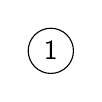
\begin{tikzpicture}[->,>=stealth',level/.style={sibling distance = 5cm/#1,
      level distance = 1.5cm}] 

      \node [arn_n] {1};
    \end{tikzpicture}
    \caption{A node}
    \label{fig:anode}
  \end{subfigure}
  \begin{subfigure}[b]{0.49\textwidth}
    \centering
    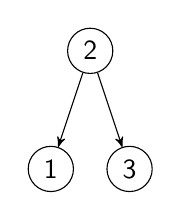
\begin{tikzpicture}[->,>=stealth',level/.style={sibling distance = 1cm/#1,
      level distance = 1.5cm}] 

      \node [arn_n] {2}
        child {
          node [arn_n] {1}
        }
        child {
          node [arn_n] {3}
        };
    \end{tikzpicture}
    \caption{A tree}
    \label{fig:atree}
  \end{subfigure}
  \caption{}
  \label{fig:nodeandtree}
\end{figure}

Trees by themselves are very open for interpretation, since they specify nothing of how keys are inserted and deleted.
An very popular variant, which we will interest ourselves in is the red-black tree~\cite{bayer1972symmetric}.
A variant of the red-black tree which we will interest ourselves in is the Okasaki variant~\cite{okasaki1999red}.
In a red-black tree, every leaf node is a node with no key or value, called an empty node.
Furthermore, in a red-black tree every node is enhanced with a color, which is either black or red, hence the name.
A red-black tree has two invariants that must be upheld.
\begin{itemize}
  \item No red node has a red parent.
  \item Every path from the root to an empty node contains the same number of black nodes.
\end{itemize}
Maintaining these two invariants, the worst case for searching becomes worse than a balanced tree, but only by a constant factor.
The shortest possible path from an empty node to a root must be the path that only contains black nodes.
The longest possible path from an empty node to the root must be the path with nodes alternating between black and red.
If all other paths than one contain only black nodes $p_1 \equiv p_2 \dots \equiv p_k$ where $p_b = (\#p_1) = (\#p_2) \dots = (\#p_k)$, where the path $p_r$ contains an alternating sequence black and red, then the worst case must be searching for last node of of $p_r$.
Visiting $p_b$ steps of $p_r$ must take us halfway since $\frac{\#p_r}{2} = p_b$ by invariant two; $\#(\textit{red}_1 \rightarrow \textit{black}_2 \dots \rightarrow \textit{red}_{p_b - 1} \rightarrow \textit{black}_{p_b})$, thus the whole path must be the double of $p_b$, $(\#p_r) = 2p_b$.
The worst case for $\#p_r$ is $n = k p_b + (\#p_r) = k p_b + 2 p_b$ and $\frac{n}{k p_b} = \#p_r$ and can be found by realizing that $p_b < \log_2 n$ such that $2p_b = (\#p_r) < 2\log_2 n$ which asymptotically becomes $\#p_r < O(2\log_2 n) = O(\log_2 n)$.

\subsubsection{Insertion}
Insertion is the first practical problem we will tackle in the red-black tree.
In~\cite{okasaki1999red} presents an elegant algorithm for insertion.
Observe that by inserting a node naively, one might violate one of the two invariants.
When we insert a node, we perform an act of \textit{rebalancing}.
Rebalancing is an action that guarantees that the tree will maintain the two aforementioned invariants after action has occurred on the tree.
When inserting a node, the node must colored red and always be placed in the bottom of the tree by searching for a position, while maintaining the ordering of the tree.
When the node has been placed, rebalancing is performed on the way back up such that violations of the two invariants, are floated up throughout the tree until the root is encountered, and then the root is colored black.
Consider that inserting a node at the leaf, may only cause a violation if the parent node of the one inserted is also red; if the parent node is black, then the invariants hold.
When considering insertion (and rebalancing), the property that the red-black tree was in a state that upheld the invariants is always maintained.
There are two types of \textit{rotations} (and two reflections for each rotation) we must perform to balance the tree after a violation.
Rotations are the act of moving nodes around such that they maintain the invariants.
Rotations are considered only for nodes that have grandparents (or conversely, nodes that have grandchildren).
For a node that has grandchildren there are four cases that may violate the invariant (again, two reflections for each rotation), which is depicted in \autoref{fig:rbrot}.
These rotations satisfy the second invariant, since for all rotations the same number of black nodes are present above \texttt{a, b, c} and \texttt{d}.
Furthermore, notice that the red node in \autoref{fig:rbrot:end} may have a red parent, this violation is only temporary, since the tree is rebalanced in reverse order of the search path.
The insertion algorithm can elegantly be encoded into the programming language, given support for nested pattern matching (\autoref{sec:remscott}).
An implementation (give that the language supports nested pattern matching) has been presented in \autoref{lst:rbimpl}.

The number of nodes to visit when searching for a position to place the new node is at most $O(\log_2 n)$ time.
The time for one \texttt{balance} is at most $1$ invocation, the \texttt{balance} function is invoked for each travelled node thus it is invoked $O(\log_2 n)$ times, which implies that the combined insertion time is $O(\log_2 n)$.

\subsubsection{Deletion}
Deletion in red-black trees is a more complicated than insertion.
Deletion of a black node can imply a much larger range of rotations than insert otherwise would.
In~\cite{germane2014deletion}, an algorithm for deletion is presented.
The algorithm, inspired by the Okasaki red-black tree, solves deletion in a similar method as insertion.
When a deletion deletes a black node, then the tree will no longer satisfy the black node invariant.
The black node invariant is then restored by introducing a double black node.
After this double black node has been introduced, a recursive algorithm, similar to the \texttt{balance} algorithm, removes all double black nodes by performing rotations.
The semantics of the rotations can be further investigated in~\cite{germane2014deletion}.

\begin{figure}[p]
  \begin{mdframed}
    \begin{subfigure}[b]{1\textwidth}
      \centering
      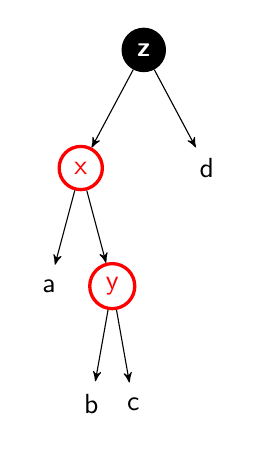
\begin{tikzpicture}[->,>=stealth',level/.style={sibling distance = 1.6cm/#1,
        level distance = 1.5cm}] 

        \node [arn_b] {z}
          child {
            node [arn_r] {x}
            child {
              node [arn_l] {a}
            }
            child {
              node [arn_r] {y}
              child {
                node [arn_l] {b}
              }
              child {
                node [arn_l] {c}
              }
            }
          }
          child {
            node [arn_l] {d}
          };
      \end{tikzpicture}
      \caption{}
      \label{fig:rbrot:c1}
    \end{subfigure}
    \begin{subfigure}[b]{1\textwidth}
      \centering
      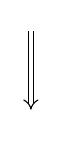
\begin{tikzpicture}
        \draw[implies-,double equal sign distance] (1,1) -- (1,2);
      \end{tikzpicture}
    \end{subfigure}

    \begin{subfigure}[b]{0.25\textwidth}
      \centering
      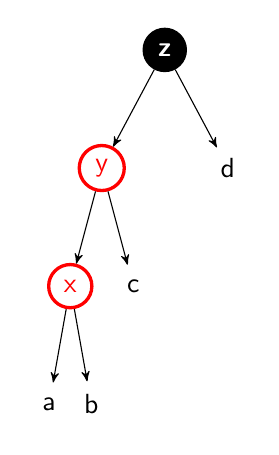
\begin{tikzpicture}[->,>=stealth',level/.style={sibling distance = 1.6cm/#1,
        level distance = 1.5cm}] 

        \node [arn_b] {z}
          child {
            node [arn_r] {y}
            child {
              node [arn_r] {x}
              child {
                node [arn_l] {a}
              }
              child {
                node [arn_l] {b}
              }
            }
            child {
              node [arn_l] {c}
            }
          }
          child {
            node [arn_l] {d}
          };
      \end{tikzpicture}
      \caption{}
      \label{fig:rbrot:c2}
    \end{subfigure}
    \begin{subfigure}[b]{0.1\textwidth}
      \centering
      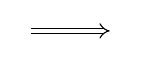
\begin{tikzpicture}
        \draw[-implies,double equal sign distance] (1,1) -- (2,1);
      \end{tikzpicture}
      \vspace*{2cm}
    \end{subfigure}
    \begin{subfigure}[b]{0.25\textwidth}
      \centering
      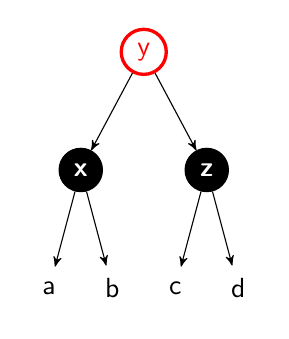
\begin{tikzpicture}[->,>=stealth',level/.style={sibling distance = 1.6cm/#1,
        level distance = 1.5cm}] 

        \node [arn_r] {y}
          child {
            node [arn_b] {x}
            child {
              node [arn_l] {a}
            }
            child {
              node [arn_l] {b}
            }
          }
          child {
            node [arn_b] {z}
            child {
              node [arn_l] {c}
            }
            child {
              node [arn_l] {d}
            }
          };
      \end{tikzpicture}
      \caption{}
      \label{fig:rbrot:end}
    \end{subfigure}
    \begin{subfigure}[b]{0.1\textwidth}
      \centering
      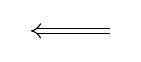
\begin{tikzpicture}
        \draw[implies-,double equal sign distance] (1,1) -- (2,1);
      \end{tikzpicture}
      \vspace*{2cm}
    \end{subfigure}
    \begin{subfigure}[b]{0.25\textwidth}
      \centering
      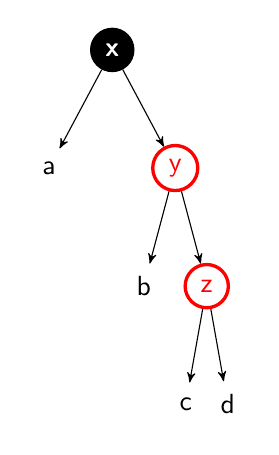
\begin{tikzpicture}[->,>=stealth',level/.style={sibling distance = 1.6cm/#1,
        level distance = 1.5cm}] 

        \node [arn_b] {x}
          child {
            node [arn_l] {a}
          }
          child {
            node [arn_r] {y}
            child {
              node [arn_l] {b}
            }
            child {
              node [arn_r] {z}
              child {
                node [arn_l] {c}
              }
              child {
                node [arn_l] {d}
              }
            }
          };
      \end{tikzpicture}
    \end{subfigure}

    \begin{subfigure}[b]{1\textwidth}
      \centering
      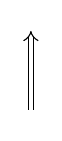
\begin{tikzpicture}
        \draw[implies-,double equal sign distance] (1,2) -- (1,1);
      \end{tikzpicture}
    \end{subfigure}
    \begin{subfigure}[b]{1\textwidth}
      \centering
      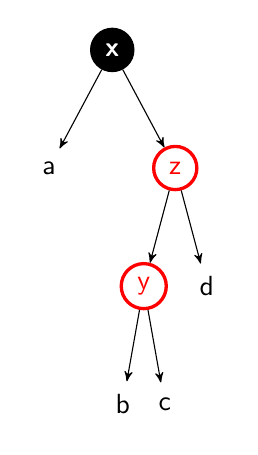
\begin{tikzpicture}[->,>=stealth',level/.style={sibling distance = 1.6cm/#1,
        level distance = 1.5cm}] 

        \node [arn_b] {x}
          child {
            node [arn_l] {a}
          }
          child {
            node [arn_r] {z}
            child {
              node [arn_r] {y}
              child {
                node [arn_l] {b}
              }
              child {
                node [arn_l] {c}
              }
            }
            child {
              node [arn_l] {d}
            }
          };
      \end{tikzpicture}
    \end{subfigure}
  \end{mdframed}
  \caption{Red-black tree rotations}
  \label{fig:rbrot}
\end{figure}


%Generally, a data structure involves two components; a shape and a set of operations.

%Data structures in traditional contexts are \textit{homogeneous} collections of data, usually with a particular shape represented by an algebraic data type, with an associated set of \textit{morphisms}.
%A homogeneous collection of data is a collection in which every element is of the same type.
%Morphisms come in various forms, they essentially encapsulate the operations that can be performed on a data structure (or more generally an object).
%Algebraic data structures and their associated morphisms come together into an algebra.
%\begin{remark}
    %In object oriented programming data structures (an algebra) is most often implemented through a class while functional programming languages often separate the shape and operations.
%\end{remark}

%Conventional data structures encapsulates data structures which are interesting under the call by value (\autoref{sec:es}) evaluation strategy.
%Evaluation strategies have many implications on the data structure in question.
%In call by name or call by need one would have to be careful not to create an unnecessary dependency which may force a computation which could otherwise stay suspended.
%The choice of evaluation strategy and data structure implementation has a significant impact on complexity analysis, which will be explored.
%
\section{Lists and immutability}
An instance of a data structure which has been thoroughly discussed throughout this thesis is \texttt{List} (\autoref{lst:listadt}).
\texttt{List} is an excellent choice as an introductory data structure since it gives insight into some very universal problems regarding both immutable and mutable data structures.
One is free to choose the operations for \texttt{List} but some common ones include \texttt{filter} (\autoref{lst:filter}) and \texttt{map} (\autoref{lst:map}).
\begin{lstlisting}[float,language=ML,caption={Filtering some \texttt{l:List a} based on a predicate p},label={lst:filter},mathescape=true]
fun filter l p = 
    match l
        | Cons x xs -> 
            let tail = filter xs p;
            if (p x)
                Cons x tail;
            else
                tail;
            ;
        | Nil -> l;
    ;
\end{lstlisting}
\begin{lstlisting}[float,language=ML,caption={Mapping from \texttt{List a} to \texttt{List b}},label={lst:map},mathescape=true]
fun map l f = 
   match l
    | Cons x xs -> Cons (f x) (map xs f);
    | Nil -> l;
   ;
\end{lstlisting}
Under the condition of immutability there are several guarantees and 



%\bibliography{bib.bib}{}
%\bibliographystyle{plain}
\printbibliography

\documentclass[11pt,oneside,a4paper]{report}

\begin{document}
\clearpage
\chapter{Appendix}

\documentclass[11pt,oneside,a4paper]{report}

\begin{document}
\begin{lstlisting}[breaklines=true,caption={The output of an exponential type},label=lst:appedix:bigexp]
########## tuple ##########
substitution set Map(c0 -> (a0 -> (b0 -> d0)))
type (a0 -> (b0 -> ((a0 -> (b0 -> d0)) -> d0)))
Type vars in sub = 4
########## tuple ##########
########## one ##########
substitution set Map(c0 -> (a0 -> (b0 -> d0)), e0 -> (h0 -> (i0 -> ((h0 -> (i0 -> j0)) -> j0))), f0 -> (k0 -> (l0 -> ((k0 -> (l0 -> m0)) -> m0))), n0 -> (((h0 -> (i0 -> ((h0 -> (i0 -> j0)) -> j0))) -> ((k0 -> (l0 -> ((k0 -> (l0 -> m0)) -> m0))) -> g0)) ->
g0))
type (((h0 -> (i0 -> ((h0 -> (i0 -> j0)) -> j0))) -> ((k0 -> (l0 -> ((k0 -> (l0 -> m0)) -> m0))) -> g0)) -> g0)
current env is Map(tuple -> Scheme(Set(a0, b0, d0),(a0 -> (b0 -> ((a0 -> (b0 -> d0)) -> d0)))), one -> Scheme(Set(k0, g0, h0, i0, l0, m0, j0),(((h0 -> (i0 -> ((h0 -> (i0 -> j0)) -> j0))) -> ((k0 -> (l0 -> ((k0 -> (l0 -> m0)) -> m0))) -> g0)) -> g0)))
Type vars = 14
Type vars in sub = 33
########## one ##########
########## two ##########
substitution set Map(o0 -> (((t0 -> (u0 -> ((t0 -> (u0 -> x0)) -> x0))) -> ((r0 -> (v0 -> ((r0 -> (v0 -> w0)) -> w0))) -> s0)) -> s0), e0 -> (h0 -> (i0 -> ((h0 -> (i0 -> j0)) -> j0))), f0 -> (k0 -> (l0 -> ((k0 -> (l0 -> m0)) -> m0))), p0 -> (((a1 -> (b1 ->
 ((a1 -> (b1 -> e1)) -> e1))) -> ((y0 -> (c1 -> ((y0 -> (c1 -> d1)) -> d1))) -> z0)) -> z0), n0 -> (((h0 -> (i0 -> ((h0 -> (i0 -> j0)) -> j0))) -> ((k0 -> (l0 -> ((k0 -> (l0 -> m0)) -> m0))) -> g0)) -> g0), c0 -> (a0 -> (b0 -> d0)), f1 -> (((((t0 -> (u0 ->
 ((t0 -> (u0 -> x0)) -> x0))) -> ((r0 -> (v0 -> ((r0 -> (v0 -> w0)) -> w0))) -> s0)) -> s0) -> ((((a1 -> (b1 -> ((a1 -> (b1 -> e1)) -> e1))) -> ((y0 -> (c1 -> ((y0 -> (c1 -> d1)) -> d1))) -> z0)) -> z0) -> q0)) -> q0))
type (((((t0 -> (u0 -> ((t0 -> (u0 -> x0)) -> x0))) -> ((r0 -> (v0 -> ((r0 -> (v0 -> w0)) -> w0))) -> s0)) -> s0) -> ((((a1 -> (b1 -> ((a1 -> (b1 -> e1)) -> e1))) -> ((y0 -> (c1 -> ((y0 -> (c1 -> d1)) -> d1))) -> z0)) -> z0) -> q0)) -> q0)
current env is Map(tuple -> Scheme(Set(a0, b0, d0),(a0 -> (b0 -> ((a0 -> (b0 -> d0)) -> d0)))), one -> Scheme(Set(k0, g0, h0, i0, l0, m0, j0),(((h0 -> (i0 -> ((h0 -> (i0 -> j0)) -> j0))) -> ((k0 -> (l0 -> ((k0 -> (l0 -> m0)) -> m0))) -> g0)) -> g0)), two -
> Scheme(Set(u0, x0, q0, a1, b1, s0, e1, d1, z0, w0, y0, v0, t0, c1, r0),(((((t0 -> (u0 -> ((t0 -> (u0 -> x0)) -> x0))) -> ((r0 -> (v0 -> ((r0 -> (v0 -> w0)) -> w0))) -> s0)) -> s0) -> ((((a1 -> (b1 -> ((a1 -> (b1 -> e1)) -> e1))) -> ((y0 -> (c1 -> ((y0 ->
 (c1 -> d1)) -> d1))) -> z0)) -> z0) -> q0)) -> q0)))
Type vars = 32
Type vars in sub = 94
########## two ##########
########## three ##########
substitution set Map(o0 -> (((t0 -> (u0 -> ((t0 -> (u0 -> x0)) -> x0))) -> ((r0 -> (v0 -> ((r0 -> (v0 -> w0)) -> w0))) -> s0)) -> s0), e0 -> (h0 -> (i0 -> ((h0 -> (i0 -> j0)) -> j0))), n2 -> (((((((v1 -> (j1 -> ((v1 -> (j1 -> k1)) -> k1))) -> ((x1 -> (u1 -
> ((x1 -> (u1 -> s1)) -> s1))) -> o1)) -> o1) -> ((((m1 -> (n1 -> ((m1 -> (n1 -> p1)) -> p1))) -> ((t1 -> (w1 -> ((t1 -> (w1 -> q1)) -> q1))) -> r1)) -> r1) -> l1)) -> l1) -> ((((((k2 -> (y1 -> ((k2 -> (y1 -> z1)) -> z1))) -> ((m2 -> (j2 -> ((m2 -> (j2 ->
h2)) -> h2))) -> d2)) -> d2) -> ((((b2 -> (c2 -> ((b2 -> (c2 -> e2)) -> e2))) -> ((i2 -> (l2 -> ((i2 -> (l2 -> f2)) -> f2))) -> g2)) -> g2) -> a2)) -> a2) -> i1)) -> i1), f0 -> (k0 -> (l0 -> ((k0 -> (l0 -> m0)) -> m0))), p0 -> (((a1 -> (b1 -> ((a1 -> (b1 -
> e1)) -> e1))) -> ((y0 -> (c1 -> ((y0 -> (c1 -> d1)) -> d1))) -> z0)) -> z0), n0 -> (((h0 -> (i0 -> ((h0 -> (i0 -> j0)) -> j0))) -> ((k0 -> (l0 -> ((k0 -> (l0 -> m0)) -> m0))) -> g0)) -> g0), c0 -> (a0 -> (b0 -> d0)), g1 -> (((((v1 -> (j1 -> ((v1 -> (j1 -
> k1)) -> k1))) -> ((x1 -> (u1 -> ((x1 -> (u1 -> s1)) -> s1))) -> o1)) -> o1) -> ((((m1 -> (n1 -> ((m1 -> (n1 -> p1)) -> p1))) -> ((t1 -> (w1 -> ((t1 -> (w1 -> q1)) -> q1))) -> r1)) -> r1) -> l1)) -> l1), h1 -> (((((k2 -> (y1 -> ((k2 -> (y1 -> z1)) -> z1))
) -> ((m2 -> (j2 -> ((m2 -> (j2 -> h2)) -> h2))) -> d2)) -> d2) -> ((((b2 -> (c2 -> ((b2 -> (c2 -> e2)) -> e2))) -> ((i2 -> (l2 -> ((i2 -> (l2 -> f2)) -> f2))) -> g2)) -> g2) -> a2)) -> a2), f1 -> (((((t0 -> (u0 -> ((t0 -> (u0 -> x0)) -> x0))) -> ((r0 -> (
v0 -> ((r0 -> (v0 -> w0)) -> w0))) -> s0)) -> s0) -> ((((a1 -> (b1 -> ((a1 -> (b1 -> e1)) -> e1))) -> ((y0 -> (c1 -> ((y0 -> (c1 -> d1)) -> d1))) -> z0)) -> z0) -> q0)) -> q0))
type (((((((v1 -> (j1 -> ((v1 -> (j1 -> k1)) -> k1))) -> ((x1 -> (u1 -> ((x1 -> (u1 -> s1)) -> s1))) -> o1)) -> o1) -> ((((m1 -> (n1 -> ((m1 -> (n1 -> p1)) -> p1))) -> ((t1 -> (w1 -> ((t1 -> (w1 -> q1)) -> q1))) -> r1)) -> r1) -> l1)) -> l1) -> ((((((k2 ->
 (y1 -> ((k2 -> (y1 -> z1)) -> z1))) -> ((m2 -> (j2 -> ((m2 -> (j2 -> h2)) -> h2))) -> d2)) -> d2) -> ((((b2 -> (c2 -> ((b2 -> (c2 -> e2)) -> e2))) -> ((i2 -> (l2 -> ((i2 -> (l2 -> f2)) -> f2))) -> g2)) -> g2) -> a2)) -> a2) -> i1)) -> i1)
current env is Map(tuple -> Scheme(Set(a0, b0, d0),(a0 -> (b0 -> ((a0 -> (b0 -> d0)) -> d0)))), one -> Scheme(Set(k0, g0, h0, i0, l0, m0, j0),(((h0 -> (i0 -> ((h0 -> (i0 -> j0)) -> j0))) -> ((k0 -> (l0 -> ((k0 -> (l0 -> m0)) -> m0))) -> g0)) -> g0)), two -
> Scheme(Set(u0, x0, q0, a1, b1, s0, e1, d1, z0, w0, y0, v0, t0, c1, r0),(((((t0 -> (u0 -> ((t0 -> (u0 -> x0)) -> x0))) -> ((r0 -> (v0 -> ((r0 -> (v0 -> w0)) -> w0))) -> s0)) -> s0) -> ((((a1 -> (b1 -> ((a1 -> (b1 -> e1)) -> e1))) -> ((y0 -> (c1 -> ((y0 ->
 (c1 -> d1)) -> d1))) -> z0)) -> z0) -> q0)) -> q0)), three -> Scheme(Set(j2, i1, m1, c2, n1, r1, z1, g2, q1, s1, w1, t1, f2, x1, o1, j1, i2, a2, h2, b2, u1, v1, p1, k2, m2, l2, l1, y1, e2, k1, d2),(((((((v1 -> (j1 -> ((v1 -> (j1 -> k1)) -> k1))) -> ((x1 -
> (u1 -> ((x1 -> (u1 -> s1)) -> s1))) -> o1)) -> o1) -> ((((m1 -> (n1 -> ((m1 -> (n1 -> p1)) -> p1))) -> ((t1 -> (w1 -> ((t1 -> (w1 -> q1)) -> q1))) -> r1)) -> r1) -> l1)) -> l1) -> ((((((k2 -> (y1 -> ((k2 -> (y1 -> z1)) -> z1))) -> ((m2 -> (j2 -> ((m2 ->
(j2 -> h2)) -> h2))) -> d2)) -> d2) -> ((((b2 -> (c2 -> ((b2 -> (c2 -> e2)) -> e2))) -> ((i2 -> (l2 -> ((i2 -> (l2 -> f2)) -> f2))) -> g2)) -> g2) -> a2)) -> a2) -> i1)) -> i1)))
Type vars = 66
Type vars in sub = 219
########## three ##########
########## four ##########
substitution set Map(o0 -> (((t0 -> (u0 -> ((t0 -> (u0 -> x0)) -> x0))) -> ((r0 -> (v0 -> ((r0 -> (v0 -> w0)) -> w0))) -> s0)) -> s0), b5 -> (((((((((m3 -> (g3 -> ((m3 -> (g3 -> u3)) -> u3))) -> ((e3 -> (l3 -> ((e3 -> (l3 -> a3)) -> a3))) -> f3)) -> f3) ->
 ((((t2 -> (v2 -> ((t2 -> (v2 -> n3)) -> n3))) -> ((c3 -> (b3 -> ((c3 -> (b3 -> z2)) -> z2))) -> w2)) -> w2) -> r3)) -> r3) -> ((((((o3 -> (s3 -> ((o3 -> (s3 -> x2)) -> x2))) -> ((p3 -> (r2 -> ((p3 -> (r2 -> j3)) -> j3))) -> v3)) -> v3) -> ((((k3 -> (u2 ->
 ((k3 -> (u2 -> t3)) -> t3))) -> ((h3 -> (q3 -> ((h3 -> (q3 -> d3)) -> d3))) -> y2)) -> y2) -> i3)) -> i3) -> s2)) -> s2) -> ((((((((r4 -> (l4 -> ((r4 -> (l4 -> z4)) -> z4))) -> ((j4 -> (q4 -> ((j4 -> (q4 -> f4)) -> f4))) -> k4)) -> k4) -> ((((y3 -> (a4 ->
 ((y3 -> (a4 -> s4)) -> s4))) -> ((h4 -> (g4 -> ((h4 -> (g4 -> e4)) -> e4))) -> b4)) -> b4) -> w4)) -> w4) -> ((((((t4 -> (x4 -> ((t4 -> (x4 -> c4)) -> c4))) -> ((u4 -> (w3 -> ((u4 -> (w3 -> o4)) -> o4))) -> a5)) -> a5) -> ((((p4 -> (z3 -> ((p4 -> (z3 -> y
4)) -> y4))) -> ((m4 -> (v4 -> ((m4 -> (v4 -> i4)) -> i4))) -> d4)) -> d4) -> n4)) -> n4) -> x3)) -> x3) -> q2)) -> q2), o2 -> (((((((m3 -> (g3 -> ((m3 -> (g3 -> u3)) -> u3))) -> ((e3 -> (l3 -> ((e3 -> (l3 -> a3)) -> a3))) -> f3)) -> f3) -> ((((t2 -> (v2 -
> ((t2 -> (v2 -> n3)) -> n3))) -> ((c3 -> (b3 -> ((c3 -> (b3 -> z2)) -> z2))) -> w2)) -> w2) -> r3)) -> r3) -> ((((((o3 -> (s3 -> ((o3 -> (s3 -> x2)) -> x2))) -> ((p3 -> (r2 -> ((p3 -> (r2 -> j3)) -> j3))) -> v3)) -> v3) -> ((((k3 -> (u2 -> ((k3 -> (u2 ->
t3)) -> t3))) -> ((h3 -> (q3 -> ((h3 -> (q3 -> d3)) -> d3))) -> y2)) -> y2) -> i3)) -> i3) -> s2)) -> s2), e0 -> (h0 -> (i0 -> ((h0 -> (i0 -> j0)) -> j0))), n2 -> (((((((v1 -> (j1 -> ((v1 -> (j1 -> k1)) -> k1))) -> ((x1 -> (u1 -> ((x1 -> (u1 -> s1)) -> s1)
)) -> o1)) -> o1) -> ((((m1 -> (n1 -> ((m1 -> (n1 -> p1)) -> p1))) -> ((t1 -> (w1 -> ((t1 -> (w1 -> q1)) -> q1))) -> r1)) -> r1) -> l1)) -> l1) -> ((((((k2 -> (y1 -> ((k2 -> (y1 -> z1)) -> z1))) -> ((m2 -> (j2 -> ((m2 -> (j2 -> h2)) -> h2))) -> d2)) -> d2)
 -> ((((b2 -> (c2 -> ((b2 -> (c2 -> e2)) -> e2))) -> ((i2 -> (l2 -> ((i2 -> (l2 -> f2)) -> f2))) -> g2)) -> g2) -> a2)) -> a2) -> i1)) -> i1), f0 -> (k0 -> (l0 -> ((k0 -> (l0 -> m0)) -> m0))), p0 -> (((a1 -> (b1 -> ((a1 -> (b1 -> e1)) -> e1))) -> ((y0 -> (
c1 -> ((y0 -> (c1 -> d1)) -> d1))) -> z0)) -> z0), n0 -> (((h0 -> (i0 -> ((h0 -> (i0 -> j0)) -> j0))) -> ((k0 -> (l0 -> ((k0 -> (l0 -> m0)) -> m0))) -> g0)) -> g0), c0 -> (a0 -> (b0 -> d0)), g1 -> (((((v1 -> (j1 -> ((v1 -> (j1 -> k1)) -> k1))) -> ((x1 -> (
u1 -> ((x1 -> (u1 -> s1)) -> s1))) -> o1)) -> o1) -> ((((m1 -> (n1 -> ((m1 -> (n1 -> p1)) -> p1))) -> ((t1 -> (w1 -> ((t1 -> (w1 -> q1)) -> q1))) -> r1)) -> r1) -> l1)) -> l1), h1 -> (((((k2 -> (y1 -> ((k2 -> (y1 -> z1)) -> z1))) -> ((m2 -> (j2 -> ((m2 ->
(j2 -> h2)) -> h2))) -> d2)) -> d2) -> ((((b2 -> (c2 -> ((b2 -> (c2 -> e2)) -> e2))) -> ((i2 -> (l2 -> ((i2 -> (l2 -> f2)) -> f2))) -> g2)) -> g2) -> a2)) -> a2), p2 -> (((((((r4 -> (l4 -> ((r4 -> (l4 -> z4)) -> z4))) -> ((j4 -> (q4 -> ((j4 -> (q4 -> f4))
-> f4))) -> k4)) -> k4) -> ((((y3 -> (a4 -> ((y3 -> (a4 -> s4)) -> s4))) -> ((h4 -> (g4 -> ((h4 -> (g4 -> e4)) -> e4))) -> b4)) -> b4) -> w4)) -> w4) -> ((((((t4 -> (x4 -> ((t4 -> (x4 -> c4)) -> c4))) -> ((u4 -> (w3 -> ((u4 -> (w3 -> o4)) -> o4))) -> a5))
-> a5) -> ((((p4 -> (z3 -> ((p4 -> (z3 -> y4)) -> y4))) -> ((m4 -> (v4 -> ((m4 -> (v4 -> i4)) -> i4))) -> d4)) -> d4) -> n4)) -> n4) -> x3)) -> x3), f1 -> (((((t0 -> (u0 -> ((t0 -> (u0 -> x0)) -> x0))) -> ((r0 -> (v0 -> ((r0 -> (v0 -> w0)) -> w0))) -> s0))
 -> s0) -> ((((a1 -> (b1 -> ((a1 -> (b1 -> e1)) -> e1))) -> ((y0 -> (c1 -> ((y0 -> (c1 -> d1)) -> d1))) -> z0)) -> z0) -> q0)) -> q0))
type (((((((((m3 -> (g3 -> ((m3 -> (g3 -> u3)) -> u3))) -> ((e3 -> (l3 -> ((e3 -> (l3 -> a3)) -> a3))) -> f3)) -> f3) -> ((((t2 -> (v2 -> ((t2 -> (v2 -> n3)) -> n3))) -> ((c3 -> (b3 -> ((c3 -> (b3 -> z2)) -> z2))) -> w2)) -> w2) -> r3)) -> r3) -> ((((((o3
-> (s3 -> ((o3 -> (s3 -> x2)) -> x2))) -> ((p3 -> (r2 -> ((p3 -> (r2 -> j3)) -> j3))) -> v3)) -> v3) -> ((((k3 -> (u2 -> ((k3 -> (u2 -> t3)) -> t3))) -> ((h3 -> (q3 -> ((h3 -> (q3 -> d3)) -> d3))) -> y2)) -> y2) -> i3)) -> i3) -> s2)) -> s2) -> ((((((((r4
-> (l4 -> ((r4 -> (l4 -> z4)) -> z4))) -> ((j4 -> (q4 -> ((j4 -> (q4 -> f4)) -> f4))) -> k4)) -> k4) -> ((((y3 -> (a4 -> ((y3 -> (a4 -> s4)) -> s4))) -> ((h4 -> (g4 -> ((h4 -> (g4 -> e4)) -> e4))) -> b4)) -> b4) -> w4)) -> w4) -> ((((((t4 -> (x4 -> ((t4 ->
 (x4 -> c4)) -> c4))) -> ((u4 -> (w3 -> ((u4 -> (w3 -> o4)) -> o4))) -> a5)) -> a5) -> ((((p4 -> (z3 -> ((p4 -> (z3 -> y4)) -> y4))) -> ((m4 -> (v4 -> ((m4 -> (v4 -> i4)) -> i4))) -> d4)) -> d4) -> n4)) -> n4) -> x3)) -> x3) -> q2)) -> q2)
current env is Map(four -> Scheme(Set(s4, q4, y4, d3, t4, g3, r2, k3, w2, x3, y2, r3, c3, m4, i4, w3, v4, u4, u3, w4, r4, z2, i3, u2, y3, a5, s2, g4, f3, t2, n3, l3, v3, c4, f4, x4, x2, h4, j3, t3, z4, e3, m3, n4, h3, v2, s3, e4, o4, z3, k4, b4, b3, j4, a3
, q2, l4, q3, a4, p4, p3, d4, o3),(((((((((m3 -> (g3 -> ((m3 -> (g3 -> u3)) -> u3))) -> ((e3 -> (l3 -> ((e3 -> (l3 -> a3)) -> a3))) -> f3)) -> f3) -> ((((t2 -> (v2 -> ((t2 -> (v2 -> n3)) -> n3))) -> ((c3 -> (b3 -> ((c3 -> (b3 -> z2)) -> z2))) -> w2)) -> w2
) -> r3)) -> r3) -> ((((((o3 -> (s3 -> ((o3 -> (s3 -> x2)) -> x2))) -> ((p3 -> (r2 -> ((p3 -> (r2 -> j3)) -> j3))) -> v3)) -> v3) -> ((((k3 -> (u2 -> ((k3 -> (u2 -> t3)) -> t3))) -> ((h3 -> (q3 -> ((h3 -> (q3 -> d3)) -> d3))) -> y2)) -> y2) -> i3)) -> i3)
-> s2)) -> s2) -> ((((((((r4 -> (l4 -> ((r4 -> (l4 -> z4)) -> z4))) -> ((j4 -> (q4 -> ((j4 -> (q4 -> f4)) -> f4))) -> k4)) -> k4) -> ((((y3 -> (a4 -> ((y3 -> (a4 -> s4)) -> s4))) -> ((h4 -> (g4 -> ((h4 -> (g4 -> e4)) -> e4))) -> b4)) -> b4) -> w4)) -> w4)
-> ((((((t4 -> (x4 -> ((t4 -> (x4 -> c4)) -> c4))) -> ((u4 -> (w3 -> ((u4 -> (w3 -> o4)) -> o4))) -> a5)) -> a5) -> ((((p4 -> (z3 -> ((p4 -> (z3 -> y4)) -> y4))) -> ((m4 -> (v4 -> ((m4 -> (v4 -> i4)) -> i4))) -> d4)) -> d4) -> n4)) -> n4) -> x3)) -> x3) ->
 q2)) -> q2)), three -> Scheme(Set(j2, i1, m1, c2, n1, r1, z1, g2, q1, s1, w1, t1, f2, x1, o1, j1, i2, a2, h2, b2, u1, v1, p1, k2, m2, l2, l1, y1, e2, k1, d2),(((((((v1 -> (j1 -> ((v1 -> (j1 -> k1)) -> k1))) -> ((x1 -> (u1 -> ((x1 -> (u1 -> s1)) -> s1))) -
> o1)) -> o1) -> ((((m1 -> (n1 -> ((m1 -> (n1 -> p1)) -> p1))) -> ((t1 -> (w1 -> ((t1 -> (w1 -> q1)) -> q1))) -> r1)) -> r1) -> l1)) -> l1) -> ((((((k2 -> (y1 -> ((k2 -> (y1 -> z1)) -> z1))) -> ((m2 -> (j2 -> ((m2 -> (j2 -> h2)) -> h2))) -> d2)) -> d2) ->
((((b2 -> (c2 -> ((b2 -> (c2 -> e2)) -> e2))) -> ((i2 -> (l2 -> ((i2 -> (l2 -> f2)) -> f2))) -> g2)) -> g2) -> a2)) -> a2) -> i1)) -> i1)), two -> Scheme(Set(u0, x0, q0, a1, b1, s0, e1, d1, z0, w0, y0, v0, t0, c1, r0),(((((t0 -> (u0 -> ((t0 -> (u0 -> x0))
-> x0))) -> ((r0 -> (v0 -> ((r0 -> (v0 -> w0)) -> w0))) -> s0)) -> s0) -> ((((a1 -> (b1 -> ((a1 -> (b1 -> e1)) -> e1))) -> ((y0 -> (c1 -> ((y0 -> (c1 -> d1)) -> d1))) -> z0)) -> z0) -> q0)) -> q0)), tuple -> Scheme(Set(a0, b0, d0),(a0 -> (b0 -> ((a0 -> (b0
 -> d0)) -> d0)))), one -> Scheme(Set(k0, g0, h0, i0, l0, m0, j0),(((h0 -> (i0 -> ((h0 -> (i0 -> j0)) -> j0))) -> ((k0 -> (l0 -> ((k0 -> (l0 -> m0)) -> m0))) -> g0)) -> g0)))
Type vars = 132
Type vars in sub = 472
########## four ##########
########## main ##########
substitution set Map(o0 -> (((t0 -> (u0 -> ((t0 -> (u0 -> x0)) -> x0))) -> ((r0 -> (v0 -> ((r0 -> (v0 -> w0)) -> w0))) -> s0)) -> s0), b5 -> (((((((((m3 -> (g3 -> ((m3 -> (g3 -> u3)) -> u3))) -> ((e3 -> (l3 -> ((e3 -> (l3 -> a3)) -> a3))) -> f3)) -> f3) ->
 ((((t2 -> (v2 -> ((t2 -> (v2 -> n3)) -> n3))) -> ((c3 -> (b3 -> ((c3 -> (b3 -> z2)) -> z2))) -> w2)) -> w2) -> r3)) -> r3) -> ((((((o3 -> (s3 -> ((o3 -> (s3 -> x2)) -> x2))) -> ((p3 -> (r2 -> ((p3 -> (r2 -> j3)) -> j3))) -> v3)) -> v3) -> ((((k3 -> (u2 ->
 ((k3 -> (u2 -> t3)) -> t3))) -> ((h3 -> (q3 -> ((h3 -> (q3 -> d3)) -> d3))) -> y2)) -> y2) -> i3)) -> i3) -> s2)) -> s2) -> ((((((((r4 -> (l4 -> ((r4 -> (l4 -> z4)) -> z4))) -> ((j4 -> (q4 -> ((j4 -> (q4 -> f4)) -> f4))) -> k4)) -> k4) -> ((((y3 -> (a4 ->
 ((y3 -> (a4 -> s4)) -> s4))) -> ((h4 -> (g4 -> ((h4 -> (g4 -> e4)) -> e4))) -> b4)) -> b4) -> w4)) -> w4) -> ((((((t4 -> (x4 -> ((t4 -> (x4 -> c4)) -> c4))) -> ((u4 -> (w3 -> ((u4 -> (w3 -> o4)) -> o4))) -> a5)) -> a5) -> ((((p4 -> (z3 -> ((p4 -> (z3 -> y
4)) -> y4))) -> ((m4 -> (v4 -> ((m4 -> (v4 -> i4)) -> i4))) -> d4)) -> d4) -> n4)) -> n4) -> x3)) -> x3) -> q2)) -> q2), o2 -> (((((((m3 -> (g3 -> ((m3 -> (g3 -> u3)) -> u3))) -> ((e3 -> (l3 -> ((e3 -> (l3 -> a3)) -> a3))) -> f3)) -> f3) -> ((((t2 -> (v2 -
> ((t2 -> (v2 -> n3)) -> n3))) -> ((c3 -> (b3 -> ((c3 -> (b3 -> z2)) -> z2))) -> w2)) -> w2) -> r3)) -> r3) -> ((((((o3 -> (s3 -> ((o3 -> (s3 -> x2)) -> x2))) -> ((p3 -> (r2 -> ((p3 -> (r2 -> j3)) -> j3))) -> v3)) -> v3) -> ((((k3 -> (u2 -> ((k3 -> (u2 ->
t3)) -> t3))) -> ((h3 -> (q3 -> ((h3 -> (q3 -> d3)) -> d3))) -> y2)) -> y2) -> i3)) -> i3) -> s2)) -> s2), e0 -> (h0 -> (i0 -> ((h0 -> (i0 -> j0)) -> j0))), n2 -> (((((((v1 -> (j1 -> ((v1 -> (j1 -> k1)) -> k1))) -> ((x1 -> (u1 -> ((x1 -> (u1 -> s1)) -> s1)
)) -> o1)) -> o1) -> ((((m1 -> (n1 -> ((m1 -> (n1 -> p1)) -> p1))) -> ((t1 -> (w1 -> ((t1 -> (w1 -> q1)) -> q1))) -> r1)) -> r1) -> l1)) -> l1) -> ((((((k2 -> (y1 -> ((k2 -> (y1 -> z1)) -> z1))) -> ((m2 -> (j2 -> ((m2 -> (j2 -> h2)) -> h2))) -> d2)) -> d2)
 -> ((((b2 -> (c2 -> ((b2 -> (c2 -> e2)) -> e2))) -> ((i2 -> (l2 -> ((i2 -> (l2 -> f2)) -> f2))) -> g2)) -> g2) -> a2)) -> a2) -> i1)) -> i1), f0 -> (k0 -> (l0 -> ((k0 -> (l0 -> m0)) -> m0))), p0 -> (((a1 -> (b1 -> ((a1 -> (b1 -> e1)) -> e1))) -> ((y0 -> (
c1 -> ((y0 -> (c1 -> d1)) -> d1))) -> z0)) -> z0), n0 -> (((h0 -> (i0 -> ((h0 -> (i0 -> j0)) -> j0))) -> ((k0 -> (l0 -> ((k0 -> (l0 -> m0)) -> m0))) -> g0)) -> g0), c0 -> (a0 -> (b0 -> d0)), g1 -> (((((v1 -> (j1 -> ((v1 -> (j1 -> k1)) -> k1))) -> ((x1 -> (
u1 -> ((x1 -> (u1 -> s1)) -> s1))) -> o1)) -> o1) -> ((((m1 -> (n1 -> ((m1 -> (n1 -> p1)) -> p1))) -> ((t1 -> (w1 -> ((t1 -> (w1 -> q1)) -> q1))) -> r1)) -> r1) -> l1)) -> l1), h1 -> (((((k2 -> (y1 -> ((k2 -> (y1 -> z1)) -> z1))) -> ((m2 -> (j2 -> ((m2 ->
(j2 -> h2)) -> h2))) -> d2)) -> d2) -> ((((b2 -> (c2 -> ((b2 -> (c2 -> e2)) -> e2))) -> ((i2 -> (l2 -> ((i2 -> (l2 -> f2)) -> f2))) -> g2)) -> g2) -> a2)) -> a2), p2 -> (((((((r4 -> (l4 -> ((r4 -> (l4 -> z4)) -> z4))) -> ((j4 -> (q4 -> ((j4 -> (q4 -> f4))
-> f4))) -> k4)) -> k4) -> ((((y3 -> (a4 -> ((y3 -> (a4 -> s4)) -> s4))) -> ((h4 -> (g4 -> ((h4 -> (g4 -> e4)) -> e4))) -> b4)) -> b4) -> w4)) -> w4) -> ((((((t4 -> (x4 -> ((t4 -> (x4 -> c4)) -> c4))) -> ((u4 -> (w3 -> ((u4 -> (w3 -> o4)) -> o4))) -> a5))
-> a5) -> ((((p4 -> (z3 -> ((p4 -> (z3 -> y4)) -> y4))) -> ((m4 -> (v4 -> ((m4 -> (v4 -> i4)) -> i4))) -> d4)) -> d4) -> n4)) -> n4) -> x3)) -> x3), f1 -> (((((t0 -> (u0 -> ((t0 -> (u0 -> x0)) -> x0))) -> ((r0 -> (v0 -> ((r0 -> (v0 -> w0)) -> w0))) -> s0))
 -> s0) -> ((((a1 -> (b1 -> ((a1 -> (b1 -> e1)) -> e1))) -> ((y0 -> (c1 -> ((y0 -> (c1 -> d1)) -> d1))) -> z0)) -> z0) -> q0)) -> q0))
type Int
current env is Map(four -> Scheme(Set(s4, q4, y4, d3, t4, g3, r2, k3, w2, x3, y2, r3, c3, m4, i4, w3, v4, u4, u3, w4, r4, z2, i3, u2, y3, a5, s2, g4, f3, t2, n3, l3, v3, c4, f4, x4, x2, h4, j3, t3, z4, e3, m3, n4, h3, v2, s3, e4, o4, z3, k4, b4, b3, j4, a3
, q2, l4, q3, a4, p4, p3, d4, o3),(((((((((m3 -> (g3 -> ((m3 -> (g3 -> u3)) -> u3))) -> ((e3 -> (l3 -> ((e3 -> (l3 -> a3)) -> a3))) -> f3)) -> f3) -> ((((t2 -> (v2 -> ((t2 -> (v2 -> n3)) -> n3))) -> ((c3 -> (b3 -> ((c3 -> (b3 -> z2)) -> z2))) -> w2)) -> w2
) -> r3)) -> r3) -> ((((((o3 -> (s3 -> ((o3 -> (s3 -> x2)) -> x2))) -> ((p3 -> (r2 -> ((p3 -> (r2 -> j3)) -> j3))) -> v3)) -> v3) -> ((((k3 -> (u2 -> ((k3 -> (u2 -> t3)) -> t3))) -> ((h3 -> (q3 -> ((h3 -> (q3 -> d3)) -> d3))) -> y2)) -> y2) -> i3)) -> i3)
-> s2)) -> s2) -> ((((((((r4 -> (l4 -> ((r4 -> (l4 -> z4)) -> z4))) -> ((j4 -> (q4 -> ((j4 -> (q4 -> f4)) -> f4))) -> k4)) -> k4) -> ((((y3 -> (a4 -> ((y3 -> (a4 -> s4)) -> s4))) -> ((h4 -> (g4 -> ((h4 -> (g4 -> e4)) -> e4))) -> b4)) -> b4) -> w4)) -> w4)
-> ((((((t4 -> (x4 -> ((t4 -> (x4 -> c4)) -> c4))) -> ((u4 -> (w3 -> ((u4 -> (w3 -> o4)) -> o4))) -> a5)) -> a5) -> ((((p4 -> (z3 -> ((p4 -> (z3 -> y4)) -> y4))) -> ((m4 -> (v4 -> ((m4 -> (v4 -> i4)) -> i4))) -> d4)) -> d4) -> n4)) -> n4) -> x3)) -> x3) ->
 q2)) -> q2)), three -> Scheme(Set(j2, i1, m1, c2, n1, r1, z1, g2, q1, s1, w1, t1, f2, x1, o1, j1, i2, a2, h2, b2, u1, v1, p1, k2, m2, l2, l1, y1, e2, k1, d2),(((((((v1 -> (j1 -> ((v1 -> (j1 -> k1)) -> k1))) -> ((x1 -> (u1 -> ((x1 -> (u1 -> s1)) -> s1))) -
> o1)) -> o1) -> ((((m1 -> (n1 -> ((m1 -> (n1 -> p1)) -> p1))) -> ((t1 -> (w1 -> ((t1 -> (w1 -> q1)) -> q1))) -> r1)) -> r1) -> l1)) -> l1) -> ((((((k2 -> (y1 -> ((k2 -> (y1 -> z1)) -> z1))) -> ((m2 -> (j2 -> ((m2 -> (j2 -> h2)) -> h2))) -> d2)) -> d2) ->
((((b2 -> (c2 -> ((b2 -> (c2 -> e2)) -> e2))) -> ((i2 -> (l2 -> ((i2 -> (l2 -> f2)) -> f2))) -> g2)) -> g2) -> a2)) -> a2) -> i1)) -> i1)), two -> Scheme(Set(u0, x0, q0, a1, b1, s0, e1, d1, z0, w0, y0, v0, t0, c1, r0),(((((t0 -> (u0 -> ((t0 -> (u0 -> x0))
-> x0))) -> ((r0 -> (v0 -> ((r0 -> (v0 -> w0)) -> w0))) -> s0)) -> s0) -> ((((a1 -> (b1 -> ((a1 -> (b1 -> e1)) -> e1))) -> ((y0 -> (c1 -> ((y0 -> (c1 -> d1)) -> d1))) -> z0)) -> z0) -> q0)) -> q0)), main -> Scheme(Set(),Int), tuple -> Scheme(Set(a0, b0, d0
),(a0 -> (b0 -> ((a0 -> (b0 -> d0)) -> d0)))), one -> Scheme(Set(k0, g0, h0, i0, l0, m0, j0),(((h0 -> (i0 -> ((h0 -> (i0 -> j0)) -> j0))) -> ((k0 -> (l0 -> ((k0 -> (l0 -> m0)) -> m0))) -> g0)) -> g0)))
Type vars = 132
Type vars = 132
Type vars in sub = 472
########## main ##########
\end{lstlisting}
\end{document}
\end{lstlisting}
\end{document}



\documentclass[11pt,oneside,a4paper]{report}

\begin{document}
\begin{align}
    &\lambda f_1 . \lambda f_2 . \lambda f_3 . (f_1 f_2) f_3 \label{eq:evaltime}\\
    =&\lambda f_1 . \lambda f_2 . \sigma (\lambda f_3 . f_1 f_2) (\lambda f_3 . f_3) \tag*{} \\
    =&\lambda f_1 . \lambda f_2 . \sigma (\sigma (\lambda f_3 . f_1) (\lambda f_3 . f_2)) (\iota) \tag*{} \\
    =&\lambda f_1 . \lambda f_2 . (\sigma (\sigma (\kappa f_1) (\kappa f_2))) \iota \tag*{} \\
    =&\lambda f_1 . \sigma (\lambda f_2 . \sigma (\sigma (\kappa f_1) (\kappa f_2))) (\lambda f_2 . \iota) \tag*{} \\
    =&\lambda f_1 . \sigma (\sigma (\lambda f_2 . \sigma) (\lambda f_2 . (\sigma (\kappa f_1)) (\kappa f_2))) (\lambda f_2 . \iota) \tag*{} \\
    =&\lambda f_1 . \sigma (\sigma (\kappa \sigma) (\sigma (\lambda f_2 . \sigma (\kappa f_1)) (\lambda f_2 . \kappa f_2))) (\lambda f_2 . \iota) \tag*{} \\
    =&\lambda f_1 . \sigma (\sigma (\kappa \sigma) (\sigma (\sigma (\lambda f_2 . \sigma) (\lambda f_2 . \kappa f_1)) (\sigma (\lambda f_2 . \kappa) (\lambda f_2 . f_2 )))) (\kappa \iota) \tag*{} \\
    =&\lambda f_1 . \sigma (\sigma (\kappa \sigma) (\sigma (\sigma (\kappa \sigma) (\sigma (\lambda f_2 . \kappa) (\lambda f_2 . f_1))) (\sigma (\kappa \kappa) (\iota)))) (\kappa \iota) \tag*{} \\
    =&\lambda f_1 . \sigma (\sigma (\kappa \sigma) (\sigma (\sigma (\kappa \sigma) (\sigma (\kappa \kappa) (\kappa f_1))) (\sigma (\kappa \kappa) (\iota)))) (\kappa \iota) \tag*{} \\
    =&\lambda f_1 . (\sigma (\sigma (\kappa \sigma) (\sigma (\sigma (\kappa \sigma) (\sigma (\kappa \kappa) (\kappa f_1))) (\sigma (\kappa \kappa) (\iota))))) (\kappa \iota) \tag*{} \\
    =&\sigma ((\lambda f_1 . \sigma) (\lambda f_1 . (\sigma (\kappa \sigma)) (\sigma (\sigma (\kappa \sigma) (\sigma (\kappa \kappa) (\kappa f_1))) (\sigma (\kappa \kappa) (\iota))))) (\lambda f_1 . \kappa \iota) \tag*{} \\
    =&\sigma ((\kappa \sigma) (\sigma (\lambda f_1 . \sigma (\kappa \sigma)) (\lambda f_1 . (\sigma (\sigma (\kappa \sigma) (\sigma (\kappa \kappa) (\kappa f_1)))) (\sigma (\kappa \kappa) (\iota))))) (\sigma (\lambda f_1 . \kappa) (\lambda f_1 . \iota)) \tag*{} \\
    =&\sigma ((\kappa \sigma) (\sigma ((\lambda f_1 . \sigma) (\lambda f_1 . \kappa \sigma)) (\sigma (\lambda f_1 .\sigma (\sigma (\kappa \sigma) (\sigma (\kappa \kappa) (\kappa f_1)))) (\lambda f_1 . (\sigma (\kappa \kappa)) (\iota))))) (\sigma (\kappa \kappa) (\kappa \iota)) \tag*{} \\
    =&\sigma  \tag*{} \\
    &((\kappa \sigma) (\sigma ((\kappa \sigma) (\sigma (\lambda f_1 . \kappa) (\lambda f_1 . \sigma))) (\sigma (\sigma (\lambda f_1 . \sigma) (\lambda f_1 . (\sigma (\kappa \sigma)) (\sigma (\kappa \kappa) (\kappa f_1)))) (\sigma (\lambda f_1 . \sigma (\kappa \kappa)) (\lambda f_1 . \iota))))) \tag*{} \\
    &(\sigma (\kappa \kappa) (\kappa \iota)) \tag*{} \\
    =&\sigma  \tag*{} \\
    &((\kappa \sigma) (\sigma ((\kappa \sigma) (\sigma (\kappa \kappa) (\kappa \sigma))) (\sigma (\sigma (\kappa \sigma) (\sigma (\lambda f_1 . \sigma (\kappa \sigma)) (\lambda f_1 . (\sigma (\kappa \kappa)) (\kappa f_1)))) (\sigma (\sigma (\kappa \sigma) ((\kappa \kappa) (\kappa \kappa))) (\kappa \iota))))) \tag*{} \\
    &(\sigma (\kappa \kappa) (\kappa \iota)) \tag*{} \\
    =&\sigma  \tag*{} \\
    &((\kappa \sigma) (\sigma ((\kappa \sigma) (\sigma (\kappa \kappa) (\kappa \sigma))) (\sigma (\sigma (\kappa \sigma) (\sigma (\sigma (\lambda f_1 . \sigma) (\lambda f_1 . \kappa \sigma)) \tag*{} \\
    &(\sigma (\lambda f_1 . \sigma (\kappa \kappa)) (\lambda f_1 . \kappa f_1)))) (\sigma (\sigma (\kappa \sigma) ((\kappa \kappa) (\kappa \kappa))) (\kappa \iota))))) \tag*{} \\
    &(\sigma (\kappa \kappa) (\kappa \iota)) \tag*{} \\
    =&\sigma  \tag*{} \\
    &((\kappa \sigma) (\sigma ((\kappa \sigma) (\sigma (\kappa \kappa) (\kappa \sigma))) (\sigma (\sigma (\kappa \sigma) (\sigma (\sigma (\kappa \sigma) ((\kappa \kappa) (\kappa \sigma))) \tag*{} \\
    &(\sigma (\sigma (\lambda f_1 . \sigma) (\lambda f_1 . \kappa \kappa)) (\sigma (\lambda f_1 . \kappa) (\lambda f_1 . f_1))))) (\sigma (\sigma (\kappa \sigma) ((\kappa \kappa) (\kappa \kappa))) (\kappa \iota))))) \tag*{} \\
    &(\sigma (\kappa \kappa) (\kappa \iota)) \tag*{} \\
    =&\sigma  \tag*{} \\
    &((\kappa \sigma) (\sigma ((\kappa \sigma) (\sigma (\kappa \kappa) (\kappa \sigma))) (\sigma (\sigma (\kappa \sigma) (\sigma (\sigma (\kappa \sigma) ((\kappa \kappa) (\kappa \sigma))) \tag*{} \\
    &(\sigma (\sigma (\kappa \sigma) ((\kappa \kappa) (\kappa \kappa))) (\sigma (\kappa \kappa) (\iota))))) (\sigma (\sigma (\kappa \sigma) ((\kappa \kappa) (\kappa \kappa))) (\kappa \iota))))) \tag*{} \\
    &(\sigma (\kappa \kappa) (\kappa \iota)) \tag*{} \\
    =&S  \tag*{} \\
    &((K S) (S ((K S) (S (K K) (K S))) (S (S (K S) (S (S (K S) ((K K) (K S))) \tag*{} \\
    &(S (S (K S) ((K K) (K K))) (S (K K) (I))))) (S (S (K S) ((K K) (K K))) (K I))))) \tag*{} \\
    &(S (K K) (K I)) \tag*{} \\
\end{align}
\end{document}

\end{document}


\end{document}
